\documentclass{article}

\usepackage{ICLR2026/iclr2026_conference,times}
% \iclrpreprintcopy
% \usepackage{natbib}
% \usepackage[T1]{fontenc}    % use 8-bit T1 fonts
\usepackage{hyperref}       % hyperlinks
\usepackage{url}            % simple URL typesetting
\usepackage{mathtools}
\usepackage{booktabs}       % professional-quality tables
\usepackage{amsfonts}       % blackboard math symbols
\usepackage{nicefrac}       % compact symbols for 1/2, etc.
\usepackage{microtype}      % microtypography
\usepackage[table]{xcolor}  % colors
\usepackage[acronym]{glossaries}
% \usepackage[utf8]{inputenc} % allow utf-8 input
% \usepackage[T1]{fontenc}    % use 8-bit T1 fonts
\usepackage{wrapfig}
\usepackage{amsthm}
\usepackage{subcaption}
\usepackage{lipsum}
% \usepackage{fancyhdr}       % header
\usepackage{amsmath}
\usepackage{graphicx}       % graphics
\usepackage{cleveref}

% Tell cleveref what to call appendices
\crefname{appendix}{Appendix}{Appendices}
\Crefname{appendix}{Appendix}{Appendices}

\makeatletter
\AddToHook{cmd/appendix/before}{%
  % From here on, sections/subsections are treated as "appendix" type
  \def\cref@section@alias{appendix}%
  \def\cref@subsection@alias{appendix}%
}
\makeatother

\usepackage{dirtytalk}
\usepackage{fp}
\usepackage{float}
\usepackage{placeins}
\usepackage{enumitem}

\usepackage{multirow}
\usepackage{etoc} % in preamble


% If glossaries ends up in PDF strings (bookmarks), disable expansion there:
\pdfstringdefDisableCommands{%
  \def\gls#1{#1}\def\Gls#1{#1}\def\glspl#1{#1}\def\Glspl#1{#1}%
}
% Also avoid hyperlinking glossary entries during triage:
\makeatletter
\@ifpackageloaded{glossaries}{\glsdisablehyper}{}%
\makeatother

\makeglossaries
\glsdisablehyper

% General terms
\newacronym{sota}{SOTA}{state-of-the-art}
\newacronym{ad}{AD}{auto-differentiation}

% Molecular Dynamics
\newacronym{lj}{LJ}{Lennard-Jones}

% Stochastic Processes
\newacronym{fbm}{fBM}{fractional brownian motion}
\newacronym{rl}{RL}{Riemann-Liouville}
\newacronym{ou}{OU}{Ornstein-Uhlenbeck}

% Stochastic Volatility Models
\newacronym{rbergomi}{rBergomi}{rough Bergomi}

% Loss Functions
\newacronym{rge}{RGE}{rotational geodesic error}
\newacronym{mse}{MSE}{mean squared error}
\newacronym{mmd}{MMD}{maximum mean discrepancy}

% Differential Equations
\newacronym{ode}{ODE}{ordinary differential equation}
\newacronym{pde}{PDE}{partial differential equation}
\newacronym{sde}{SDE}{stochastic differential equation}
\newacronym{cde}{CDE}{controlled differential equation}
\newacronym{yde}{YDE}{Young differential equation}
\newacronym{rde}{RDE}{rough differential equation}
\newacronym{rsde}{RSDE}{rough stochastic differential equation}
\newacronym{spde}{SPDE}{stochastic partial differential equation}

% Integrators
\newacronym{rk}{RK}{Runge--Kutta}
\newacronym{rkmk}{RKMK}{Runge--Kutta--Munthe--Kaas}

% Other functions
\newacronym{sg}{SG}{Savitzky--Golay}

% Neural Differential Equations
\newacronym{node}{NODE}{neural ordinary differential equation}
\newacronym{ncde}{NCDE}{neural controlled differential equation}
\newacronym{nrde}{NRDE}{neural rough differential equation}
\newacronym{bnrde}{B-NRDE}{branched neural rough differential equation}

% Neural SPDEs
\newacronym{nspde}{NSPDE}{neural stochastic partial differential equation}
\newacronym{dlrnet}{DLR-Net}{Deep Latent Regularity Net}
\newacronym{nors}{NORS}{Neural Operator with Regularity Structure}

% Hopf Algebras
\newacronym{gl}{GL}{Grossman--Larson}
\newacronym{bck}{BCK}{Butcher--Connes--Kreimer}
\newacronym{mkw}{MKW}{Munthe--Kaas--Wright}

% Cheminformatics
\newacronym{smiles}{SMILES}{Simplified Molecular-input Line-entry System}
\newacronym{dft}{DFT}{density functional theory}
\newacronym{md}{MD}{molecular dynamics}

% Graph theory
\newacronym{spdgraph}{SPD}{shorest path distance}

% Differential Geometry
\newacronym{spdman}{SPD}{symmetric positive definite}
\newacronym{aiman}{AI}{affine invariant}
\newacronym{bw}{BW}{Bures-Wasserstein}

% NNs
\newacronym{mlp}{MLP}{multilayer perceptron}
\newacronym{nlp}{NLP}{natural language processing}
\newacronym{llm}{LLM}{large language models}
\newacronym{ffn}{FFN}{feedforward neural network}
\newacronym{cnn}{CNN}{convolutional neural network}
\newacronym{mpnn}{MPNN}{message passing neural network}

% Training
\newacronym{mt}{MT}{multitask}
\newacronym{zs}{ZS}{zero-shot}

% Activations
\newacronym{relu}{ReLU}{rectified linear unit}
\newacronym{gelu}{GELU}{Gaussian error linear unit}
\newacronym{silu}{SiLU}{sigmoid linear unit}

% GNNs
\newacronym{gnn}{GNN}{graph neural network}
\newacronym{gtn}{GTN}{graph transformer neural network}
\newacronym{egnn}{EGNN}{Equivariant Graph Neural Network}
\newacronym{gat}{GAT}{graph attention network}
\newacronym{gatv2}{GATv2}{graph attention network v2}

% Transformer Elements
\newacronym{mha}{MHA}{multi-headed scaled dot-product attention}
\newacronym{rope}{RoPE}{Rotary Position Embedding}
\newacronym{trope}{T-RoPE}{Temporal Rotary Position Embedding}
\newacronym{nope}{NoPE}{no positional encoding}

% Graph Neural Network Elements
\newacronym{rwpe}{RWPE}{random walk positional encoding}
\newacronym{rrwp}{RRWP}{relative random walk probabilities}

% Neural Operators
\newacronym{no}{NO}{neural operator}
\newacronym{atoms}{ATOM}{Atomistic Transformer Operator for Molecules}
\newacronym{fno}{FNO}{Fourier Neural Operator}
\newacronym{egno}{EGNO}{Equivariant Graph Neural Operator}
\newacronym{gnot}{GNOT}{General Neural Operator Transformer}
\newacronym{hnca}{HNCA}{Heterogenous Normalised Cross-Attention}

% Hypothesis Tests
\newacronym{ks}{KS}{Kolmogorov-Smirnov}

% Datasets
\newacronym{omd}{OMD}{Oxford Multi-motion Dataset}
 

\let\origcite\cite
\let\cite\citep
\let\textcite\citet



\newtheorem{theorem}{Theorem}[section]
\newtheorem{corollary}{Corollary}[theorem]
\newtheorem{lemma}[theorem]{Lemma}
\newtheorem{proposition}[theorem]{Proposition}
\newtheorem{definition}[theorem]{Definition}


\newcommand{\EScomment}[1]{{\color{blue}ES:  #1}}
\newcommand{\AHcomment}[1]{{\color{purple}AH: #1}}

\newcommand{\revision}[1]{{\color{purple} #1}}


\hypersetup{colorlinks=true,linkcolor=red!70!black,linktocpage=false,citebordercolor=blue!70!black,citecolor=blue!70!black,anchorcolor=blue!70!black}

\title{ATOM: A Pretrained Neural Operator for\\ Multitask Molecular Dynamics}
\author{Luke Thompson \\
  % The University of Sydney Business School \\
  The University of Sydney
  % Camperdown, NSW 2006, Australia\\
  % \texttt{luke.thompson@sydney.edu.au} \\
  \And
  Davy Guan \\
  Data61 CSIRO 
  % CSIRO \\
  % Sydney\\
  % \texttt{davy.guan@data61.csiro.au} \\
  \And
  Dai Shi \\
  University of Cambridge
  % The University of Sydney Business School \\
  % The University of Sydney \\
  % Camperdown, NSW 2006, Australia\\
  % \texttt{email@email} \\
  \And
  Slade Matthews\thanks{These authors contributed equally as senior authors.} \\
  % Sydney Pharmacy School \\
  The University of Sydney 
  % Camperdown, NSW 2006, Australia\\
  % \texttt{slade.matthews@sydney.edu.au} \\  
  \And
  Junbin Gao\footnotemark[1] \\
  % The University of Sydney Business School \\
  The University of Sydney 
  % Camperdown, NSW 2006, Australia\\
  % \texttt{junbin.gao@sydney.edu.au} \\
  \And
  Andi Han\footnotemark[1] \ \thanks{Correspondence to: \texttt{andi.han@sydney.edu.au}.} \\
  % School of Mathematics and Statistics \\
  The University of Sydney 
  % \texttt{andi.han@sydney.edu.au} \\
}



\iclrfinalcopy 

\begin{document}

\maketitle
\thispagestyle{fancy}
\pagestyle{fancy}
\lhead{Published as a conference paper at ICLR 2026}
\begin{abstract}
% \Gls{md} simulations underpin modern computational drug discovery, materials science, and biochemistry. However, existing methods are notoriously expensive and time-consuming. In this light, we propose \gls{atoms}, a pretrained transformer neural operator for modeling 3D point cloud dynamics with a particular focus on predicting \gls{md} trajectories. \gls{atoms} shows excellent zero-shot generalization to unseen chemical compounds, demonstrating an average improvement of 44\% over state-of-the-art equivariant graph baselines in multi-timestep atom-position \gls{mse}. To facilitate multitask operator learning, we introduce TG80, the largest multi-compound \gls{md} benchmark dataset to date, comprising over 2.5 million femtoseconds of simulation data across 80 diverse compounds. Additionally, \gls{atoms} advances state-of-the-art performance on established single-task \gls{md} benchmarks, reducing \gls{mse} by 19\% on MD17 and 13\% on RMD17. Our methodology capitalizes upon recent advancements in transformer pretraining (i.e., Muon, RoPE) and requires no prior knowledge of graph structure, unlike existing message-passing approaches. With \gls{atoms}, TG80, and the release of numerous pretrained checkpoints, we lay the groundwork for future research into \gls{md} neural operators with concrete scientific applicability.

\Gls{md} simulations underpin modern computational drug discovery, materials science, and biochemistry. Recent machine learning models provide high-fidelity \gls{md} predictions without the need to repeatedly solve quantum mechanical forces, enabling significant speedups over conventional pipelines. Yet many such methods typically enforce strict equivariance and rely on sequential rollouts, thus limiting their flexibility and simulation efficiency. They are also commonly single-task, trained on individual molecules and fixed timeframes, which restricts generalization to unseen compounds and extended timesteps. To address these issues, we propose \gls{atoms}, a pretrained transformer neural operator for multitask molecular dynamics. \gls{atoms} adopts a quasi-equivariant design that requires no explicit molecular graph and employs a temporal attention mechanism, enabling accurate parallel decoding of multiple future states. To support operator pretraining across chemicals and timescales, we curate TG80, a large, diverse, and numerically stable \gls{md} dataset with over 2.5 million femtoseconds of trajectories across 80 compounds. \gls{atoms} achieves state-of-the-art performance on established single-task benchmarks, such as MD17, RMD17 and MD22. After multitask pretraining on TG80, \gls{atoms} shows exceptional zero-shot generalization to unseen molecules across varying time horizons. We believe \gls{atoms} represents a significant step toward accurate, efficient, and transferable molecular dynamics models.

% \textbf{\gls{atoms} Code: \url{https://github.com/luke-a-thompson/gtno_py}} \\
% \textbf{\gls{atoms} Code: In supplementaries} \\
% \textbf{TG80 Dataset: In supplementaries}
\end{abstract}



 \addtocontents{toc}{\protect\setcounter{tocdepth}{-1}}
\section{Introduction}   
\glsresetall

% \AHcomment{Potential road map for introduction:
% \begin{enumerate}
%     \item Introduce the context of molecule dynamics (why it matters). 
%     \item The issues with existing methods (include both classic simulations and neural methods). \textbf{Autoregressive} and \textbf{equivariance} are two main issues! 
%     \begin{itemize}
%         \item The problem with autoregressive includes error accumulation and slow inference time 
        
%         \item  For equivariance, find references that state equivariance is key to generalization for geometric dynamics \cite{xu_equivariant_2024,han2024geometric}
        
%         \item The problem with equivariance involves potentially higher computational cost (spherical haromonics, higher-order symmetry); also restrict the expressive power with highly constrained designs to preserve symmetry
%     \end{itemize}
%     \item Introduce the limitation of single-task, i.e., models need to train on each molecule for their trajectory prediction.
    
%     \item Introduce ATOM as the first quasi-equivariant pre-trained framework for molecule dynamics, and achieve good zero-shot generalizability across both molecules and timeframes 
%     \begin{itemize}
%         \item We model molecules as point clouds and introduce graph only for positional encoding. Thus we allow flexible model design .
%     \end{itemize}
% \end{enumerate}    
% }

\Gls{md} serves as a computational microscope of atomic motion and is now integral to drug discovery and materials science pipelines \cite{dror_biomolecular_2012, de_vivo_role_2016}. In ab initio molecular dynamics, quantum-mechanical \gls{dft} is used to compute atomic forces, and the resulting equations of motion are integrated to generate high-fidelity trajectories. However, \gls{dft}'s computational complexity scales at least cubically with the number of atoms, and relies on double-precision arithmetic that limits GPU acceleration \cite{kresse_efficiency_1996, stein_double-hybrid_2020, li_scaling_2024}. 

Neural approaches have recently emerged as a promising solution to the scalability bottleneck. \textit{Equivariant} architectures, in particular, encode physical symmetries to model interatomic dynamics, achieving ab initio-level accuracy at significantly reduced computational cost  \cite{batzner_e3-equivariant_2022, musaelian_learning_2022, batatia_design_2022, batatia_mace_2023, xu_equivariant_2024}. While equivariance is often deemed essential for improving generalization, strict symmetry preservation involves substantial tradeoffs \cite{xu_equivariant_2024, schreiner_implicit_2023}. Architectures that enforce exact equivariance at every layer often increase computational overhead, restrict model expressivity, and complicate optimization \cite{fuchs_se3-transformers_2020, brehmer_geometric_2023, elhag_relaxed_2025}. It is unclear whether symmetry constraints can be relaxed without sacrificing accuracy for molecular dynamics.

Furthermore, most existing methods for molecular dynamics are \textit{autoregressive}, predicting the next state based on the current one \citep{kohler_equivariant_2019,fuchs_se3-transformers_2020,thiemann2025force}.  Autoregressive approaches often struggle to capture long-horizon temporal dependencies and accumulate error as the prediction horizon grows \cite{bengio_scheduled_2015, bergsma_sutranets_2023, taieb_bias_2016}. Inference speeds are also constrained by the need for sequential integration, failing to exploit modern, highly parallel compute architectures. One exception is \gls{egno} \cite{xu_equivariant_2024}, which models the entire trajectory with neural operator learning. Nevertheless, \gls{egno} enforces strict equivariance and is single-task in nature, i.e., it is trained and evaluated on trajectories of each molecule separately with a fixed time horizon, which limits \textit{zero-shot generalization} to unseen molecules or timeframes. 
% even though \textit{zero-shot generalization} is essential for practical drug-discovery pipelines.

\textbf{Our Main Contributions.} In this work, we address the above issues regarding equivariance, autoregression, and zero-shot generalization within a unified framework, which we call \textit{\gls{atoms}}. To this end, we propose a pre-trained neural operator with a transformer backbone for molecular dynamics and introduce a new \gls{md} dataset, TG80, which is both chemically diverse and numerically stable for multitask pretraining and benchmarking. 
\begin{itemize}[leftmargin=0.15in]
    \item \textit{Design innovations}. \gls{atoms} is \textit{quasi-equivariant} by employing an equivariant lifting layer that produces symmetry-aware features, while allowing subsequent transformer blocks to be unconstrained for flexibility and expressiveness. 
    Unlike autoregressive models, \gls{atoms} allows \textit{parallel decoding} of molecule states across multiple timesteps, directly learning the trajectory operator. By encoding time lags via a novel temporal rotary position embedding, \gls{atoms} enhances temporal interpolation and extrapolation, enabling robust predictions across multiple time horizons. Finally, \gls{atoms} requires no predefined molecular graph and operates directly on \textit{point clouds}, naturally accommodating long-range spatial interactions without the need for hand-crafted connectivity. 

    \item \textit{Performance highlights}. \gls{atoms} sets new state-of-the-art on single-task \gls{md} benchmarks. For larger, sparsely connected molecules in MD22, \gls{atoms} significantly outperforms existing graph-based baselines by capturing the long-range atomic interactions. In the multitask regime, we pretrain \gls{atoms} on TG80 trajectories from multiple molecules and varying timeframes, demonstrating significant zero-shot transfer to both unseen molecules and timesteps, reducing S2T \gls{mse} relative to \gls{egno} by 54.17\% on average. This achieves performance on par with existing specialized baselines tailored for such molecules and timeframes.  To the best of our knowledge, this is the first method that demonstrates such generalization capability in molecular dynamics.
\end{itemize}

We believe our work represents a shift in molecular dynamics modeling, where we demonstrate the potential of quasi-equivariance designs and zero-shot generalization to out-of-domain systems, which is enabled by the comprehensive TG80 \gls{md} dataset. \gls{atoms} and TG80 are available at \href{https://github.com/luke-a-thompson/ATOM}{this repository}.


 % Here, an equivariant network learns to approximate the underlying physics, which are then integrated numerically in the manner of classical \gls{dft} \cite{batzner_e3-equivariant_2022, musaelian_learning_2022, batatia_design_2022, batatia_mace_2023}. 

% Nevertheless, most existing neural methods are autoregressive , as they 

% Whilst much faster than purely numerical methods, autoregressive approaches can miss long-range temporal correlations and compound error as the step size or horizon grows \cite{bengio_scheduled_2015, bergsma_sutranets_2023, taieb_bias_2016}. Inference speeds are also constrained by the need for sequential integration, failing to capture a key advantage of modern, highly parallel compute architectures. Second, despite previous works considering equivariance essential for generalization, strict symmetry preservation involves substantial tradeoffs \cite{xu_equivariant_2024,han2024geometric, schreiner_implicit_2023}. Spherical harmonics and higher-order algebras raise computational overheads whilst restricting model expressivity and complicating optimization \cite{fuchs_se3-transformers_2020, brehmer_geometric_2023, elhag_relaxed_2025}. Recent work on hybrid equivariance has shown that, given careful model design, weak equivariance methods can achieve similar results without these tradeoffs \cite{elhag_relaxed_2025}. In these designs, the network remains unconstrained and equivariance is achieved with regularization or approximation techniques \textbf{CITE}.

% \Gls{md} neural operators have begun to address autoregression; however, current operators are strictly equivariant, and generalization to novel molecules remains an open challenge. As enabling (zero-shot) transfer learning is essential for \gls{md} operators to see practical applications in drug discovery and materials science pipelines involving new molecular structures, this naturally raises the question:

% \begin{center}
%     \textit{Can we develop a pretraining framework for scalable dynamics learning with zero-shot generalizability?}
% \end{center}

% We answer the above question affirmatively by introducing \gls{atoms}, a pre-trained neural operator for molecular dynamics, and TG80, a new multitask dataset. In particular, we highlight our \textbf{main contributions} as follows: \AHcomment{Revisit}

% to integrate with a step size beyond 10 femtoseconds would be almost unheard of, yet as readers will see in our evaluation, we routinely show results with timesteps of up to 5000 in length.


% Contemporary \gls{md} employ quantum-mechanical \gls{dft} simulations to calculate time series of atomic positions termed \textit{trajectories}. However, these methods become inefficient as number of atoms $N$ increases, with computational complexities ranging from  \(\mathcal{O}(N^3)\) to \(\mathcal{O}(N^5)\). In addition, they require double-precision floating-point computations, which limits GPU acceleration \cite{kresse_efficiency_1996, stein_double-hybrid_2020, li_scaling_2024}.

% To address these scalability issues, recent works propose neural methods for tasks traditionally in the domain of \gls{dft} simulations. Neural \gls{md} approaches typically predict single-timestep forces and energies from a snapshot molecular conformation \cite{batatia_design_2022, batzner_e3-equivariant_2022, faber_alchemical_2018, gao_torchani_2020, gasteiger_gemnet_2021, kovacs_linear_2021, musaelian_learning_2022} or diffuse low-energy conformation states \cite{gu_aligning_2024,xu_geodiff_2022}.

% Current approaches to modeling per-atom positional dynamics are autoregressive, and as such, risk failing to capture multi-timestep temporal correlations or accumulating error as trajectory length increases \cite{bengio_scheduled_2015, bergsma_sutranets_2023, taieb_bias_2016}. The inference time requirements of autoregressive methods are also naturally greater than those of a hypothetical parallel-decoding \gls{md} model.

% Thus far, \gls{md} operators are single-task learners that demonstrate limited generalization to unseen chemical compounds, restricting their real-world scientific applicability. Enabling (zero-shot) transfer learning in such models is crucial for integrating them into pipelines exploring novel molecules, which is essential for advancing material science and drug discovery. This naturally raises the question:


% capable of zero-shot generalization to unseen chemical compounds, opening a new direction in operator learning with clear scientific applicability. We also introduce TG80, a new multitask \gls{MD} dataset. Beyond \gls{atoms} and TG80, we highlight the following \textbf{main contributions}.

% \begin{itemize}[leftmargin=0.3in]
%     \item We propose \gls{atoms}, a weakly equivariant neural operator that adapts proven \gls{nlp} techniques to operator learning, including RoPE to encode point cloud dynamics. We perform extensive ablations to guide future operator research.

%     \item We introduce TG80, a \gls{md} benchmark comprising \(>2.5\times 10^6\) fs of trajectories across 80 compounds for multi-task \gls{md} learning; it offers greater chemical diversity and improved numerical stability than prior benchmarks and is released under the MIT licence.

%     \item Our proposed method, \gls{atoms}, achieves \gls{sota} \textit{single-task} performance on both our new dataset and the existing MD17 and RMD17 benchmarks, showing average improvement of \(19.21\%\) and \(12.99\%\), respectively across various compounds. 

%     \item We pre-train \gls{atoms} on TG80, and demonstrate significant zero-shot generalizability to unseen compounds, achieving performance parity with existing single-task baselines despite never seeing them in training. To the best of our knowledge, this is the first method that successfully demonstrates such generalization capability in molecular dynamics learning.

%     % \item We novelly adapt \gls{nlp} strategies to operator learning, such as \gls{rope}, to encode temporal point cloud dynamics, and perform extensive ablations to evidence these changes and guide future neural operator research.
%     \item We make pretrained \gls{atoms} checkpoints and our new dataset TG80 publicly available (upon acceptance), to establish a robust platform to support future research into scalable and scientifically impactful neural operators for \gls{md}.
% \end{itemize}

\section{Related work}
\textbf{Equivariant Neural Networks.}
Equivariance (to transformations such as rotation, reflection, and translation) has emerged as an essential physics-informed prior for deep learning models on molecular data \cite{bronstein_geometric_2021, duval_hitchhikers_2023}. 
% As a molecule's properties remain invariant under rotation, reflection, or other transformations, it follows that its latent representations should transform in a manner that preserves these symmetries. 
Early works employed convolutional approaches to achieve translation equivariance in E(3) \cite{weiler_3d_2018, wu_pointconv_2020} or tensor product attention and spherical harmonics to enforce roto-translational equivariance in SE(3) \cite{fuchs_se3-transformers_2020,thomas_tensor_2018}. In contrast, \gls{mpnn} frameworks, such as \gls{egnn} and others \cite{garcia_satorras_en_2021, gasteiger_gemnet_2021, huang_equivariant_2022}, achieve equivariance by operating on strictly equivariant features, such as inter-node distances and directions. While effective, \glspl{mpnn} typically assume a fixed molecular graph. This is problematic when the underlying structure contains non-local interactions and dynamic bonding effects (e.g., resonances, transient interactions), which render predefined graphs inaccurate over time \cite{knutson_dynamic_2022,luo_predicting_2021}. To address this issue, we model molecules as point clouds, with our attention represented as a fully connected graph that allows unrestricted information propagation across the molecule.

% Recent approaches have explored embeddings into geometric Clifford algebras to construct equivariant representations that capture higher-order multivector symmetries not preserved by traditional equivariant networks \cite{brehmer_geometric_2023, zhdanov_clifford-steerable_2024}. Orthogonal to these developments, \textcite{elhag_relaxed_2025} shows that non-equivariant architectures can be regularized to approximate equivariance with the addition of a loss term penalizing deviation from the expected transformation behavior under a given symmetry group.

{\textbf{Time-coarsened Molecular Dynamics}
Time coarsening is a coarse-graining method which preserves molecular structure, but compresses many short integration steps into a few large-stride updates to reduce the cost of long-time simulation \cite{kmiecik_coarse-grained_2016}.
Stochastic coarse-graining approaches often learn transition kernels on configuration space, bypassing explicit integration of the equations of motion. \textcite{klein_timewarp_2023} learns such a kernel with a normalizing flow and uses it as an MCMC proposal targeting the Boltzmann distribution, \textcite{hsu_score_2024} uses a conditional diffusion model to learn a transition probability matrix, and \textcite{yu_unisim_2025} uses flow-matching to learn a vector field transporting current states to future states.
Closer to our framework, deterministic methods such as MDNet \cite{zheng_learning_2021} and TrajCast \cite{thiemann2025force} learn a GNN and \gls{egnn}, respectively, which autoregressively predict fixed strides 10-100 times larger than those of \gls{md} integrators. \textcite{bigi_flashmd_2025} incorporates Hamiltonian structure and explicit energy-conservation. Most of the methods require direct force learning and are sequential in nature, while \Gls{atoms} may be interpreted as a \textit{force-free} deterministic coarse-graining approach, wherein temporal pushforward is approximated by a learned propagation operator which is decoded \textit{in parallel}.}

\textbf{Neural Operators.}
Neural operators are deep learning methods for learning operators between function spaces \cite{kovachki_neural_2021}. 
A wide variety of architectures have been proposed for such operator learning. Notably, \gls{fno} \cite{li_fourier_2021} learns an operator in the Fourier domain, while its derivatives G-FNO \cite{helwig_group_2023} and PINO \cite{li_physics-informed_2023}, respectively, add group equivariance and physics-informed properties. \citet{xu_equivariant_2024} bridges this framework with molecular dynamics by recasting the task as learning a propagation operator that evolves historical atomic positions into their future configurations. Specifically, \gls{egno} \cite{xu_equivariant_2024} integrates \gls{egnn} and \gls{fno} layers to learn dynamic trajectories, capturing spatial and temporal correlations.
Recently, transformer neural operators \cite{bryutkin_hamlet_2024,hao_gnot_2023,li_transformer_2023} have surpassed the performance of \gls{fno} in most \gls{pde} tasks. Notably, OFormer \cite{li_transformer_2023} uses a linear Galerkin-type attention mechanism, which omits the softmax and instead interprets the latent column vectors as basis functions. \gls{gnot} \cite{hao_gnot_2023} employs a novel subquadratic cross-attention methodology to integrate multiple feature types (e.g., shape and point relationships) into their transformer blocks. With \gls{atoms}, we unify the \gls{md} problem formulation and temporal discretization approach introduced by \gls{egno} with the increased representational power of transformers in operator settings.

% Another attentional approach is HAMLET \cite{bryutkin_hamlet_2024}, which constructs a graph of input observations and iteratively updates this representation using an encoder-decoder graph transformer. 

\textbf{MD Benchmarks.}
Research on graph machine learning for molecular dynamics suffers from poor benchmarking \cite{bechler-speicher_position_2025}. 
% Research into graph learning for molecular dynamics is marred by the \say{bad benchmarking culture,} which affects \gls{gnn} literature more broadly \cite{bechler-speicher_position_2025}. 
For example, despite the fact that MD17 Benzene exhibits non-physical noise approximately 1000 times higher compared to other compounds \cite{christensen_role_2020}, it is still regularly employed to benchmark new models \cite{bihani_egraffbench_2023,huang_equivariant_2022,liao_equiformer_2023, xu_equivariant_2024}. The practical relevance of single-task learning on these datasets is also dubious, as predicting trajectories for molecules with existing numerical solutions offers minimal benefit. We believe the strengths of neural approaches emerge in transfer learning, where models generalize to unseen compounds, thereby circumventing the computational costs associated with explicit numerical simulations. This motivates our development of TG80 to facilitate multitask dynamics learning across molecular systems.



\section{Atomistic Transformer Operator for Molecules (ATOM)}
\label{sect:atom}

In this section, we first introduce the problem formulation (\Cref{sect:problem}) and then propose the framework of \gls{atoms} by introducing the key model and training designs (\Cref{sect:main_model}). We then discuss the multitask pretraining for \gls{atoms} and introduce TG80 \gls{md} dataset (\Cref{sect:multi-pretrain}).


\subsection{Problem Formulation}
\label{sect:problem}
We follow \cite{xu_equivariant_2024} to cast molecular dynamics prediction as operator learning. We model a molecule of $N$ atoms as a point cloud in $\mathbb R^3$, which we denote as $\mathcal{G}^{(t)}$ for a given system state time $t$. In particular, we write $\mathcal{G}^{(t)} = (\mathbf x_i^{(t)}, \mathbf v_i^{(t)})_{i= 1}^N$ that represent molecules in terms of the atom positions $\mathbf{x}$ and velocities $\mathbf{v}$.
% We model molecules as point clouds. Given a time $t$, a molecule is represented by $\mathcal{G}^{(t)}$. 
% We consider a system state time \(t\) as a point cloud of \(N\) nodes, which we denote $\mathcal{G}^{(t)}$. 
Our objective is to predict a future trajectory $\mathcal{G}^{(t + \Delta t)}$, where $\Delta t \in [0, \Delta T]$. 

Similar to \cite{xu_equivariant_2024}, we focus on predicting the position states only. Let $\mathcal{U} \colon [0, \Delta T] \rightarrow \mathbb R^{N \times  3}$ be the trajectory function mapping $\Delta t$ to $U(\Delta t) \in \mathbb R^{N \times  3}$ representing molecule positions $\Delta t$ in the future. We assume a solution operator $F^\dagger \colon \mathcal{G}^{(t)} \rightarrow \mathcal{U}$ exists which provides the underlying future trajectory given system states at $t$. Thus, the goal of molecular dynamics prediction becomes training a neural operator $F_\theta(\mathcal{G}^{(t)})$ to approximate the target trajectory function $F^\dagger(\mathcal{G}^{(t)})$: $\min_\theta \mathbb E_{\mathcal{G}^{(t)}} \mathcal{L} \big(F_\theta(\mathcal{G}^{(t)}) (t) , F^\dagger(\mathcal{G}^{(t)})(t) \big)$,
% \begin{equation*}
%     \min_\theta \mathbb E_{\mathcal{G}^{(t)}} \mathcal{L} \left(F_\theta(\mathcal{G}^{(t)}) (t) , F^\dagger(\mathcal{G}^{(t)})(t) \right)
% \end{equation*}
for some loss function $\mathcal{L} \colon \mathcal{U} \times \mathcal{U}\rightarrow \mathbb R$. Here, expectation is with respect to the different initial states.
By discretizing over the temporal domain and considering $L_2$ loss, we optimize the neural operator with a discretized temporal sampling of the states:
\begin{align}
    &\min_{\theta} \frac{1}{P} \sum_{p=1}^P \mathbb{E}_{\substack{
            \mathcal{G}^{(t)}  \\
            }
        } 
         \left\|
            F_\theta\left( \mathcal{G}^{(t)}  \right)(\Delta t_p) - F^\dagger \left (\mathcal{G}^{(t)} \right) (\Delta t_p)
        \right\|_{2}^{2}.
        \label{eq:objective_function}
\end{align}
where $\{ \Delta t_1, ..., \Delta t_p \}$ are discrete timesteps. We replace the true future state $F^\dagger(\mathcal{G}^{(t)})(\Delta t_p)$ with the known future ground truth node positions $\mathbf{x}^{(t+\Delta t_p)}$ for $\Delta t_p \in [0, \Delta T]$.

{
\textbf{Quasi-equivariance.}
\label{def:quasi_equivariance}
We formally define quasi-equivariance, motivated by \cite{elhag_relaxed_2025}.
\begin{definition}[$\varepsilon$-quasi-equivariance]
Let $G$ be a compact group acting on $\mathcal{X}$ and $\mathcal{Y}$ via $\phi$ and $\rho$, respectively, and let $\mathcal{D}$ be a distribution over $\mathcal{X}$. We call a function $f: \mathcal{X} \rightarrow \mathcal{Y}$ $\varepsilon$-quasi-equivariant with respect to $G$ if it satisfies $\mathbb E_{x \sim \mathcal{D}} \int_G \big\| f( \phi(g)(x) ) - \rho(g) (f(x)) \big\| \, d\mu(g) \leq \varepsilon$,
% \begin{equation*}
%     \mathbb E_{x \in \mathcal{X}} \big\|  \int_G f( \phi(g)(x) ) d \mu (g)  - \int_G \rho(g) (f(x)) d\mu(g)
%     \big\| \leq \varepsilon 
% \end{equation*}
where $\mu$ denotes the normalized Haar measure on $G$.
\end{definition}
Taking the norm inside the group integral ensures that $\varepsilon = 0$ if and only if $f(\phi(g)(x)) = \rho(g)(f(x))$ for $\mathcal{D}$-almost every $x$ and $\mu$-almost every $g$; errors under different group elements cannot cancel. In our experiments $G = \mathrm{SO}(3)$ acting by rotation on atomic positions and velocities, and we approximate the expectation and group integral by Monte Carlo (\Cref{app:quasi_equivariance_mc}).
}

\textbf{Single- and multitask.}
\label{sec:st_and_mt}
Unlike prior works \cite{schreiner_implicit_2023, xu_equivariant_2024}, we consider both single-task and multitask settings. \textit{Single-task} refers to the case where a separate model is independently trained and evaluated on each molecule and fixed timeframes. This corresponds to the conventional practice in molecular dynamics benchmarks. \textit{Multitask} instead pretrains one unified model on several molecules across varying time lags and evaluates out-of-domain trajectories on unseen molecules, thereby directly testing zero-shot cross-molecule generalization. Under a multitask setting, the objective \eqref{eq:objective_function} computes the expectation over trajectories of multiple molecules. 




% {\color{purple}
% comprising a sequence of $P$ states $\{\mathcal{G}^{(t+\Delta t_p)}\}_{p=1}^{P}$ at increments $\Delta t_p$. For example, given an initial graph $\mathcal{G}^{(1000)}$ and choosing \(\Delta t = 3000, P=8\), we get the increments defined as $\Delta t_p = 3000 + (p-1)$ for $p = 1,\dots,8$. Thus, our aim is to estimate the sequence \(\{\mathcal{G}^{(4000)}, \mathcal{G}^{(4001)}, \dots, \mathcal{G}^{(4007)}\}\) using only the input state $\mathcal{G}^{(1000)}$. }
% \AHcomment{This formulation seems a little different to EGNO. If this is what we do, please justify.}

% We aim to learn a neural operator $F_\theta$ to estimate the ground-truth evolution operator $F^\dagger$ \EScomment{\cite{xu_equivariant_2024}}. Given an input $\mathcal{G}^{(t)}$, the operator predicts a future trajectory by outputting states at discrete time increments \(\{ \Delta t_p \}\). The ideal learning objective is to minimize the expected   distance between the predicted and actual future states over the trajectory horizon:
% \begin{align}
%     &\min_{\theta}\mathbb{E}_{\substack{
%             \mathcal{G}^{(t)} \sim p_\text{data} \\
%             }
%         } \frac{1}{P} \sum_{p=1}^P
%          \left\|
%             F\left( \mathcal{G}^{(t)} ; \theta \right)(\Delta t_p) - F^\dagger \left (\mathcal{G}^{(t)} \right) (\Delta t_p)
%         \right\|_{2}^{2}.
%         \label{eq:objective_function}
% \end{align}
% Focusing on positional dynamics, we replace the true future state $F^\dagger(\mathcal{G}^{(t)})(\Delta t_p)$ with the known future ground truth node positions $\mathbf{x}'_{t+\Delta t_p}$.




\subsection{ATOM Model and Training Design}
\label{sect:main_model}

% \AHcomment{Write a summary of ATOM here, which capitalizes the key components.}

Here we outline the pipeline of \gls{atoms}. At its core is an \textit{equivariant lifting} layer (\Cref{sec:equivariant_lifting}), which maps atomic positions, velocities and their phase features into a richer embedding space while preserving symmetry under the Euclidean group \(E(3)\). The lifted embeddings are then processed by the \gls{atoms} attention block, which applies \textit{heterogeneous attention} over positions, velocities, and phase features with chemical augmentation (\Cref{sect:atom_attn}).  To capture temporal dynamics, we incorporate a \textit{temporal rotary position embedding} (T-RoPE) (\Cref{sect:atom_attn}) that depends only on time lags and is shared across atoms, ensuring translation invariance in time and permutation invariance within each molecule. {The parameterized \gls{atoms} can be written by 
\begin{equation*}
    F_\theta \coloneqq \mathcal{P} \circ \sigma(\mathcal{K}_L) \circ \cdots \circ \sigma(\mathcal{K}_1) \circ \mathcal{Q}
\end{equation*}
where $\mathcal{Q}$, $\mathcal{P}$ denotes the equivariant lifting and projection operators respectively. $\mathcal{K}_l, l = 1,..., L$ are the data-dependent kernels induced by cross attention (See Appendix \ref{app:kernel}), and $\sigma$ denotes some nonlinear activation function.
}


% We highlight that layers after equivariant lifting are unconstrained, which preserves model flexibility and expressiveness. 
Finally, to counter numerical noise in training trajectories, we inject randomly sampled position and velocity perturbations during training (\Cref{sec:label_noise}), which improves robustness and acts as a regularizer against overfitting. 
The overall pipeline of \gls{atoms} is in \Cref{fig:atom-arch}. 

% We first encode the molecule's positions and velocities via an equivariant lifting and a tensor product operation, which ensures a rich embedding of the molecule's state space and preserves symmetry under $E(3)$. The lifted embedding is sent to the \gls{atoms} attention block, which allows cross-feature attention and employs a form of \gls{rope} to encode the dynamical trajectory whilst retaining permutation invariance within each point cloud. We present the complete model architecture in \Cref{fig:trope_arch}. 




\begin{figure}[t]
    \centering
    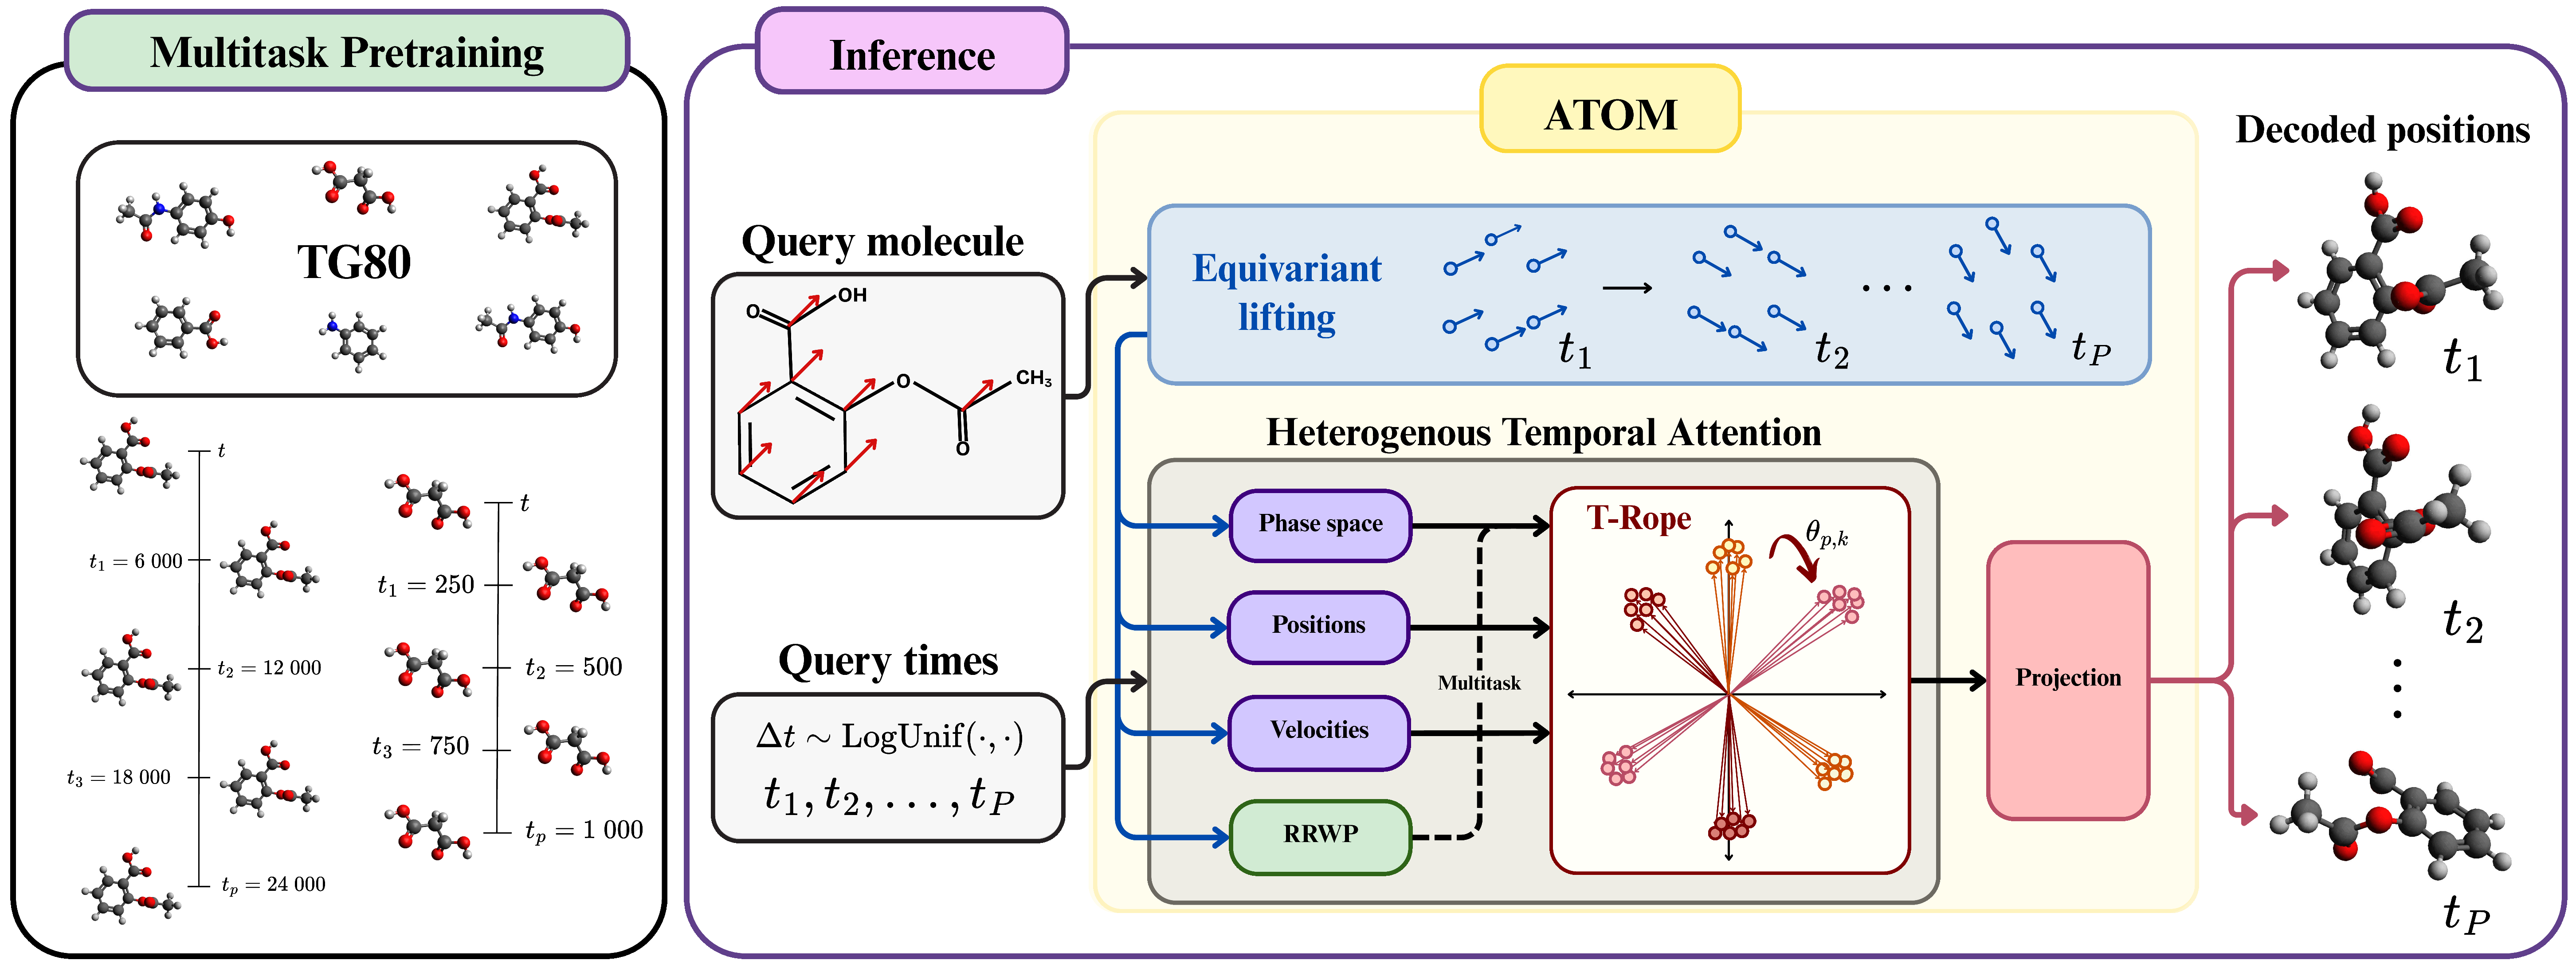
\includegraphics[width=1\linewidth]{Figures/new_architecture_camera_cropped.pdf}
    \caption{\textbf{\gls{atoms} Pipeline}. We pretrain \gls{atoms} on the TG80 dataset across multiple molecules with stochastic time lags. At inference, \gls{atoms} takes a query molecule and timestamps and directly outputs corresponding molecular states. 
    % An input compound taken \(\mathcal{G}^{(t)}\), taken at time \(t\), undergoes equivariant lifting (\Cref{sec:equivariant_lifting}), before the lifted features are passed into the heterogeneous temporal attention blocks. \Gls{trope} then rotates queries and keys in a permutation-invariant manner to encode sequence position \(P\). The angle of rotation \(\theta\) varies with \(\Delta t\). Now with temporal context, the output of the cross-attention is back to \(\mathbb{R}^3\) via a \(\mathrm{Projection}\) \gls{mlp}, producing the atom coordinates at desired query times.
    }
    \label{fig:atom-arch}
\end{figure}

\subsubsection{\textit{E}(3) Equivariant Lifting}
\label{sec:equivariant_lifting}
To model atomic states in a symmetry-respecting way, each atom is encoded with its 3D position and velocity, augmented with their norms: $\mathbf{x} = (x,y,z,\sqrt{x^2+y^2+z^2}), \, \mathbf{v} = (v_x, v_y, v_z, \sqrt{v_x^2+v_y^2+v_z^2})$.
% \begin{equation}
%     \mathbf{x} = (x,y,z,\sqrt{x^2+y^2+z^2}), \qquad \mathbf{v} = (v_x, v_y, v_z, \sqrt{v_x^2+v_y^2+v_z^2}), \notag
% \end{equation}
% These augmented vectors contain two types of geometric quantities with distinct transformation behaviors under the Euclidean group $E(3)$: (1) the positions and velocities transform equivariantly under $E(3)$ and change sign under inversion (odd parity); (2) the norms, which are invariant and have even parity. This means each input admits the irreducible representation \(V_{\text{in}} \coloneqq \rho^{\text{odd}}_1 \oplus \rho^{\text{even}}_0\) of \(E(3)\): an odd-parity vector and even-parity scalar. See \Cref{sec:group_representations} for a more detailed introduction to irreps.
To construct higher-dimensional features that remain consistent with $E(3)$ symmetry, we apply \textit{equivariant lifting} that maps the inputs through learnable functions that preserve group actions.
% Equivariant lifting embeds inputs into a higher-dimensional space via learnable maps such that the embedded features transform consistently under rotations and translations. 
% Specifically, we achieve this using \(E(3)\)-equivariant \glspl{mlp} \(f_{\mathbf{x}},f_{\mathbf{v}} \colon V_{\text{in}}\longrightarrow V\) where  \(V \coloneqq \bigoplus_{k=1}^m V_{\text{in}}\) and $m$ controls the expressivity of the the embedding space.
Specifically, we use \(E(3)\)-equivariant linear layers \cite{geiger_e3nn_2022} that lift the position and velocity vectors to a feature space
% \(f_{\mathbf{x}},f_{\mathbf{v}} \colon V_{\text{in}}\longrightarrow V\) where  \(V \coloneqq \bigoplus_{k=1}^m V_{\text{in}}\) and $m$ denotes the number of channels in the lifted space. Here $\bigoplus$ denotes the direct sum.
wherein they satisfy equivariance constraints by construction. We further construct phase space featrues for each atom by augmenting the position and velocity vectors with atomic number, which is subsequently processed by a learnable equivariant layer to obtain a lifted representation. The final lifted embedding for a molecule is given by $({\mathbf X}, {\mathbf{V}}, {\mathbf{Z}}) \in \mathbb R^{3 \times N P \times d_v}$ corresponding to position, velocity and phase features. The second dimension aggregates nodes and time for attention and $d_v$ is the embedding space dimension. 

We highlight that after the equivariant lifting layer, we do not enforce equivariance in the subsequent transformer blocks. This relaxation improves performance over fully equivariant designs while still showing robustness to random trajectory rotations versus non-equivariant baselines (see \Cref{sec:ablations}).
% We similarly obtain a symmetry-preserving representation of each atom's phase space by forming the concatenation \(\mathbf{z} = (\mathbf{x} || \mathbf{v} || \mathcal{Z}) \in W_\text{in} \coloneqq V_\text{in} \oplus V_\text{in} \oplus \rho_0^\text{even}\) and passing this through an equivariant linear layer \(f_\mathbf{z}\) to form the lifted representation \(\tilde{\mathbf{z}} \coloneqq f_\mathbf{z}(\mathbf{z})\).
% , i.e., $f_{\mathbf{x}}(g\!\cdot\!\mathbf{x}) \;=\; \rho_V(g)\, \cdot f_{\mathbf{x}}(\mathbf{x})$, $f_{\mathbf{v}}(g\!\cdot\!\mathbf{v}) \;=\; \rho_V(g)\, \cdot f_{\mathbf{v}}(\mathbf{v})$, $\forall g \in E(3)$, where $\cdot$ denotes the group action and $\rho_V(g)$ is the group action of $g$ on $V$.
% \begin{equation}
%     f_{\mathbf{x}}(g\!\cdot\!\mathbf{x}) \;=\; \rho_V(g)\, \cdot f_{\mathbf{x}}(\mathbf{x}),
%     \qquad
%     f_{\mathbf{v}}(g\!\cdot\!\mathbf{v}) \;=\; \rho_V(g)\, \cdot f_{\mathbf{v}}(\mathbf{v}), 
%     \quad 
%     \forall g \in E(3). \notag
% \end{equation}
% where $\cdot$ denotes the group action and $\rho_V(g)$ represents the group action of $g$ on $V$.


% To obtain a symmetry-consistent representation of each atom’s phase space, we enrich the velocity with chemical information, by augmenting the velocity with atomic number $\mathcal{Z}$ (an even-parity scalar): $\hat{\mathbf{v}} = (\mathbf{v}||\mathcal{Z}) \in W_\text{in} \coloneqq V_\text{in} \oplus \rho_0^\text{even}$.
% \begin{equation*}
%     \hat{\mathbf{v}} = (\mathbf{v}||\mathcal{Z}) \in W_\text{in} := V_\text{in}\oplus \rho_0^\text{even}
% \end{equation*}
% We pass this through another equivariant linear layer to form its lifted representation: $ \tilde{\mathbf{v}}^* \coloneqq f_{\hat{\mathbf{v}}}(\hat{\mathbf{v}}).$
% To form each atom's phase space vector \(\mathbf{z}\), we first form the concatenation \(\hat{\mathbf{v}} = (\mathbf{v}||\mathcal{Z}) \in W_\text{in} := V_\text{in} \oplus \rho_0^\text{even}\), where the atomic number \(\mathcal{Z} \in \mathbb{N}_{>0}\) is an even-parity scalar. We pass this through another equivariant linear layer to form its lifted representation:
% \begin{equation}
%     f_{\hat{\mathbf{v}}} \colon W_\text{in} \to V,
%     \qquad
%     \tilde{\mathbf{v}}^* \coloneqq f_{\hat{\mathbf{v}}}(\hat{\mathbf{v}}).
% \end{equation}
% {Finally, we construct a phase space embedding, where each point characterizes the complete state (positions and velocities) of a dynamical system.} 
% Then we construct a phase space embedding to characterize the complete state of our dynamical system.
% We employ a symmetry-preserving learned mixing operation \cite{thomas_tensor_2018, fuchs_se3-transformers_2020}, i.e., $\mathbf{z} = \sum_{k=1}^m W_k \Pi_k [\tilde{\mathbf{x}} \otimes \tilde{\mathbf{v}}^*]$,
% Specifically, we form the tensor product of both embeddings' irreps \(\tilde{\mathbf{x}} \otimes \tilde{\mathbf{v}}^* \in V \otimes V\), then project back to our embedding space using a Clebsch-Gordan module \(\Pi_k \colon V \otimes V \to V\) and apply weights \(W_k\):
% \begin{equation}
%     \mathbf{z} = \sum_{k=1}^m W_k \Pi_k 
%     [\tilde{\mathbf{x}} \otimes \tilde{\mathbf{v}}^*]. \notag
% \end{equation}
% where \(\Pi_k \colon V \otimes V \to V\) projects a component of the tensor product into $V$ based on Clebsch-Gordan decomposition. 


% Summation over the \(m\) irreps yields our final phase space embedding \(\mathbf{z} \in V\).

\subsubsection{ATOM Heterogeneous Temporal Attention}
\label{sect:atom_attn}

% Inspired by \cite{hao_gnot_2023}
We employ a heterogeneous temporal attention mechanism to enable mixing between multiple features $({\mathbf{X}}, {\mathbf{V}}, {\mathbf{Z}}) \in \mathbb R^{3 \times N P \times d_v}$ across spatial and temporal dimensions.
    % \EScomment{We first flatten each feature \(  F_i \in \{ \tilde{\mathbf{x}}, \tilde{\mathbf{v}}, \mathbf{z} \}\) to shape $F_i \in \mathbb{R}^{(PN) \times V}$,
% \begin{equation}
%     F_i \in \mathbb{R}^{(PN) \times V}.
% \end{equation}
% which allows our attention to mix information across the spatial \(N\) nodes and temporal \(P\) timesteps dimensions.}
\FPeval{\PctImproveCrossAttvsStdAtt}{round((5.99-5.27)/5.99*100,2)}
We use the phase space embedding ${\mathbf Z}$ as the query and attend to the key-value pairs formed from all features ${\mathbf{X}}, {\mathbf{V}}, {\mathbf{Z}} \in \mathbb R^{NP \times d_v}$. In \Cref{fig:MD17_ablation}, we show that this improves performance by \PctImproveCrossAttvsStdAtt\% over standard self-attention for single-task prediction. To encode temporal information, we introduce Temporal RoPE (T-RoPE), adapting \gls{rope} \citep{su_roformer_2023} to irregular time lags by scaling the phase rotations according to cumulative timestamps constructed from per-step increments ${ \Delta t}$.

Let the hidden dimension per head be $d_h$ (even). We define frequencies $\omega_k=b^{-2k/d_h}$ for $k=0,\dots,d_h/2-1$.
Given per-step time increments $\{\Delta t_p\}_{p=1}^{P}$, we build timestamps
$t_p=t+\sum_{r=1}^{p}\Delta t_r$, and assign a \emph{single} rotation to all $N$ atoms at timestep $p$: $\mathbf R_{p}=\operatorname{diag}\left(\mathbf R(\theta_{p,0}),\dots,\mathbf R(\theta_{p,d_h/2-1})\right) \in \mathbb R^{d_h \times d_h}$, where $\theta_{p,k}=\frac{\omega_k}{\tau}\,\bigl(t_p-t_0\bigr)$ and
% \[
% \mathbf R_{p}=\operatorname{diag}\left(\mathbf R(\theta_{p,0}),\dots,\mathbf R(\theta_{p,d_h/2-1})\right) \in \mathbb R^{d_h \times d_h},
% \quad
% \theta_{p,k}=\frac{\omega_k}{\tau}\,\bigl(t_p-t_0\bigr),
% % \quad
% % \mathbf R(\theta)=
% %     \begin{bmatrix}\cos\theta&-\sin\theta\\ \sin\theta&\cos\theta
% % \end{bmatrix},
% \]
$\mathbf R(\theta) \in \mathbb R^{2 \times 2}$ is the rotation matrix with angle $\theta$ and $\tau > 0$ is a timescale hyperparameter. Suppose the query molecule state at time $p$ is given as $\mathbf Q_p \in \mathbb R^{N \times d_h}$ and key molecule state at time $p'$ is $\mathbf K_{p'} \in \mathbb R^{N \times d_h}$. We apply $\mathbf R_p, \mathbf R_{p'}$ to $\mathbf Q_p, \mathbf K_{p'}$ respectively so that the rotary dot product $\mathbf Q_p \mathbf R_p (\mathbf K_{p'} \mathbf R_{p'})^\top$  
% \[
% \langle \mathbf R_p\,\mathbf Q,\ \mathbf R_{p'}\,\mathbf K\rangle
% =
% \sum_{k}
% (q^{(k)})^\top \mathbf R \left(\frac{\omega_k}{\tau}\,(t_{p'}-t_p)\right)\,k^{(k)},
% \]
depends only on the time interval $t_{p'}-t_p$. This makes attention \textit{translation invariant} in time, which allows for interpolation and extrapolation across irregular increments $\{\Delta t_p\}$. In addition, sharing the same $\mathbf R_p$ across all $N$ atoms in a molecule ensures \textit{permutation-invariance} within a timestep.
% (i.e., translation-invariant in time), while remaining permutation-invariant within each timestep (all $N$ atoms of a molecule share the same $\mathbf R_p$). 
For aggregated query and key matrices $\mathbf Q, \mathbf K \in \mathbb R^{NP \times d_h}$, we denote the application of temporal \gls{rope} across $P$ timesteps and $N$ atoms as $\operatorname{T-RoPE}(\mathbf Q), \operatorname{T-RoPE}(\mathbf K) \in \mathbb R^{NP \times d_h}$.

Specifically, a single-head attention layer of \gls{atoms} computes 
\begin{equation*}
    \sum_{\mathbf F   \in \{{\mathbf{X}}, {\mathbf{V}}, {\mathbf{Z}} \}} \gamma_{\mathbf F}  \, \operatorname{softmax} \Big( \frac{ \operatorname{T-RoPE}(Q({\mathbf{Z}})) \, \operatorname{T-RoPE}( K(\mathbf F) )^\top}{\sqrt{d_h}} \Big) 
     V(\mathbf F),
\end{equation*}
where $Q(\cdot), K(\cdot), V(\cdot)$ represent the query, key and value projections. 
% and $\text{T-RoPE}(\cdot)$ encodes temporal positional information across all nodes. 
We introduce learnable weights $\gamma_{\mathbf F}$ to modulate the relative importance of each feature. 
In \Cref{appx:kernel_integral_cross_att}, we show that heterogeneous attention is equivalent to a kernel integral operator and discuss its properties.



% \subsubsection{Temporal RoPE}
% \label{sec:trope}

% KEEP
% \gls{rope} \cite{su_roformer_2023} is a positional embedding where latent query \(\textbf{Q}\) and key \(\textbf{K}\) are progressively rotated according to their sequence position. 
% \AHcomment{Add some motivation related to our setting to introduce temporal RoPE}
% As \gls{rope} generally outperforms the sinusoidal positional encodings \cite{su_roformer_2023, barbero_round_2024}, which remain standard in neural operator architectures, we develop \textit{\gls{trope}}, an adaptation of \gls{rope} for dynamics learning.

% % \EScomment{\paragraph{\gls{trope} is slice-local} The datasets considered in our paper, \gls{egno} and prior works (e.g., MD17, MD22), arise from equilibrium constant-temperature \gls{md}, and thus constitute a stationary ergodic process \cite{pengmei_beyond_2024, chmiela_accurate_2023}. In fact, any frames at \(t\) and \(t+\Delta t\) are identically distributed under the Boltzmann measure as \(\Delta t \to \infty\) \cite{braun_best_2019} and thus, after equilibration, absolute timestep encodings carry little physical information. Therefore, we define the \gls{trope} rotation angle only by the relative index \(p \in \{1,\dots,P\}\) within the attention matrix:
% % \begin{equation}
% %     \theta_{p,k} = p \cdot \omega_k
% % \end{equation}
% % where the frequency \(\omega\) is defined in \Cref{eq:rope_freq}. As a secondary benefit, our approach may also mitigate the poor length generalization of many global positional encoding schemes \cite{kazemnejad_impact_2023}.}

% % While \gls{rope} rotates each token based on its absolute position in a 1D sequence, 

% KEEP
% \Gls{trope} assigns a single rotation $\mathbf R_p$ to all  \(N\) atoms at a given timestep $\Delta t_p$. This preserves permutation invariance within timesteps, while still encoding a temporal ordering. The rotations are carried out in the same manner as \gls{rope}, where the hidden features with dimension $d_h$ are split into \({d_{h}}/{2}\) disjoint 2D subspaces. Each subspace receives a unique angle \(\theta_{p,k}\) with frequency level $k$ \cite{su_roformer_2023}, yielding
% \begin{equation}
%     \mathbf R_{p}\;=\;
%     \operatorname{diag}\Bigl(\mathbf R(\theta_{p,1}),\dots, \mathbf R(\theta_{p,d_h/2})\Bigr)
%     \;\in\;
%     \mathbb{R}^{d_{h}\times d_{h}},
%     \quad
%     \mathbf R(\theta)=
%     \begin{bmatrix}
%         \cos\theta & -\sin\theta\\[2pt]
%         \sin\theta &  \cos\theta
%     \end{bmatrix}.
%     \label{eq:trope_single_angle}
% \end{equation}
% Here, we retain the orthogonality property of \gls{rope} \cite{su_roformer_2023} \(\langle \mathbf  R_p \mathbf Q, \mathbf R_p \mathbf K \rangle = \langle \mathbf Q, \mathbf  K \rangle\), ensuring temporal rotation commutes with attention. 


% \gls{rope} \cite{su_roformer_2023} encodes order by rotating queries and keys by position-dependent phases across disjoint 2D feature pairs, and empirically outperforms absolute positional encodings \citep{su_roformer_2023,barbero_round_2024}. 
% We adapt it to irregular time lags by driving the phases with \emph{timestamps} built from per-step increments $\{\Delta t_p\}$.

% Let the hidden dimension per head be $d_h$ (even). We define frequencies $\omega_k=b^{-2k/d_h}$ for $k=0,\dots,d_h/2-1$.
% Given per-step time increments $\{\Delta t_p\}_{p=1}^{P}$, we build timestamps
% $t_p=t+\sum_{r=1}^{p}\Delta t_r$, and assign a \emph{single} rotation to all $N$ atoms at timestep $p$:
% \[
% \mathbf R_{p}=\operatorname{diag}\left(\mathbf R(\theta_{p,0}),\dots,\mathbf R(\theta_{p,d_h/2-1})\right) \in \mathbb R^{d_h \times d_h},
% \quad
% \theta_{p,k}=\frac{\omega_k}{\tau}\,\bigl(t_p-t_0\bigr),
% % \quad
% % \mathbf R(\theta)=
% %     \begin{bmatrix}\cos\theta&-\sin\theta\\ \sin\theta&\cos\theta
% % \end{bmatrix},
% \]
% where $\mathbf R(\theta) \in \mathbb R^{2 \times 2}$ is the rotation matrix with angle $\theta$ and $\tau > 0$ is a timescale hyperparameter. Suppose the query molecule state at time $p$ is given as $\mathbf Q_p \in \mathbb R^{N \times d_h}$ and key molecule state at time $p'$ is $\mathbf K_{p'} \in \mathbb R^{N \times d_h}$. We apply $\mathbf R_p, \mathbf R_{p'}$ to $\mathbf Q_p, \mathbf K_{p'}$ respectively so that the rotary dot product $\mathbf Q_p \mathbf R_p (\mathbf K_{p'} \mathbf R_{p'})^\top$  
% % \[
% % \langle \mathbf R_p\,\mathbf Q,\ \mathbf R_{p'}\,\mathbf K\rangle
% % =
% % \sum_{k}
% % (q^{(k)})^\top \mathbf R \left(\frac{\omega_k}{\tau}\,(t_{p'}-t_p)\right)\,k^{(k)},
% % \]
% depends only on the time interval $t_{p'}-t_p$. This makes attention translation invariant in time, which allows for interpolation and extrapolation across irregular increments $\{\Delta t_p\}$. In addition, sharing the same $\mathbf R_p$ across all $N$ atoms in a molecule ensures permutation-invariance within a timestep.
% % (i.e., translation-invariant in time), while remaining permutation-invariant within each timestep (all $N$ atoms of a molecule share the same $\mathbf R_p$). 
% For aggregated query and key matrices $\mathbf Q, \mathbf K \in \mathbb R^{NP \times d_h}$, we denote the application of temporal \gls{rope} across $P$ timesteps and $N$ atoms as $\operatorname{T-RoPE}(\mathbf Q), \operatorname{T-RoPE}(\mathbf K) \in \mathbb R^{NP \times d_h}$.



% Different increment patterns $\{\Delta t_p\}$ therefore induce different phases and are learnable by the \gls{atoms}.

% \AHcomment{double check $d_V$, $d_h$}



% The Kronecker formulation below shows how this extends to the full attention matrix:
% \begin{equation}
%     R = \begin{bmatrix}
%     R_1\otimes I_N & \mathbf{0} & \cdots & \mathbf{0} \\[1mm]
%     \mathbf{0} & R_2\otimes I_N & \cdots & \mathbf{0} \\[1mm]
%     \vdots & \vdots & \ddots & \vdots \\[1mm]
%     \mathbf{0} & \mathbf{0} & \cdots & R_P\otimes I_N
%     \end{bmatrix} \in \mathbb{R}^{(PN \cdot d_{\text{head}}) \times (PN \cdot d_{\text{head}})},
% \end{equation}
% where \( I_N \) is the \( N \times N \) identity matrix. We avoid forming this large matrix and implement \gls{trope} element-wise, requiring only \(\mathcal{O}(PNd_\text{head})\).

% We define the frequency vector identically to \gls{rope}, where the rotation angle for each point cloud is determined by scaling the integer time index with the frequency vector 
% \begin{equation}
%     \label{eq:rope_freq}
%     \boldsymbol{\omega} = \left( \frac{1}{\text{base}^{\frac{2i}{d_{\text{head}}}}} \right)_{i=0}^{\frac{d_{\text{head}}}{2} - 1}.
% \end{equation}

% \EScomment{Shall we use $\mathcal{G}^{(t)} \in \{\mathcal{G}^{(t)}\}^P_{t=1}$.}

% \subsubsection{Heterogeneous Attention}
% \label{sec:cross_attention}

% \AHcomment{combine with temporal rope}






% and remark that our kernel fails to satisfy global Lipschitz continuity \cite{delattre_efficient_2023}


% We then compute the queries from the phase space \(\mathbf{Q} = \mathbf{z}\mathbf W_{Q} + \mathbf{b}_{Q}\) and then keys and values from the lifted positions and velocities \(\mathbf{K}_i = F_i \mathbf{W}_K + \mathbf{b}_K, \mathbf{V}_i = F_i \mathbf{W}_V + \mathbf{b}_V\), with \(\mathbf{Q}, \mathbf{K}, \mathbf{V} \in \mathbb{R}^{(PN) \times V}\).
% \begin{equation}
%     \mathbf{Q} = \mathbf{z}\mathbf W_{Q} + \mathbf{b}_{Q},
%     \qquad
%     \EScomment{\mathbf{Q} \in \mathbb{R}^{(PN) \times V}}
% \end{equation}
% then the keys \(\mathbf{K}\) and values \(\mathbf{V}\) from the lifted positions and velocities:
% \begin{equation}
%      \mathbf{K}_i = F_i \mathbf{W}_K + \mathbf{b}_K,
%      \quad 
%      \mathbf{V}_i = F_i \mathbf{W}_V + \mathbf{b}_V,
%      \qquad
%      \EScomment{\mathbf{K}, \mathbf{V} \in \mathbb{R}^{(PN) \times V}}.
% \end{equation}

% Considering the single-head case for simplicity, this yields the per-feature attention weights
% \begin{equation}
%     \mathbf{\alpha}_i
%     =
%     \operatorname{softmax} \left( \frac{ \operatorname{T-RoPE}(\mathbf{Q}) \, \operatorname{T-RoPE}(\mathbf{K}_i)^\top}{\sqrt{d_h}} \right),
%     \EScomment{\qquad a_i \in \mathbb{R}^{(PN) \times (PN)}},
% \end{equation}
% where \gls{trope} injects temporal positional information prior to softmax normalization and scaling. We then form each feature's final attention matrix as \(\mathbf{A}_i = \alpha_i\mathbf{V}_i \in \mathbb{R}^{(PN) \times V}\). \EScomment{In our attention scheme, only the phase space undergoes self-attention, when \(F_i = \mathbf{z}\), and hence \(\mathbf{Q}, \mathbf{K}, \mathbf{V}\) are all derived from \(\mathbf{z}\). All other features only undergo cross-attention, with queries from \(\mathbf{z}\) and keys/values from \(F_i\).

% To aggregate the \(M\) attention outputs \( \{ \mathbf{A}_i \}_{i=1}^M \), we learn softmax-normalized weights, \( \{\gamma_i\}_{i=1}^M \), compute a gated sum over feature attentions, then pass this through an output projection
% we learn a vector of gating logits \(\beta = [\beta_1, \dots, \beta_i]^\top \in \mathbb{R}^M\), one per feature, which are normalized via softmax into weights \( \{\gamma_i\}_{i=1}^M\) with \(\sum_i^M \gamma_i = 1\).
% We then compute the gated sum
% \begin{equation}
%     % A_\textbf{agg} = \sum_{i=1}^M \gamma_i \mathbf{A}_i
%     \mathbf{x}_\text{out}
%     =
%     \mathbf{W}_O \left(\sum_{i=1}^M \gamma_i \mathbf{A}_i \right) + \mathbf{b}_O,
%     \quad
%     \mathbf{W}_O \in \mathbb{R}^{V \times V}.
% \end{equation}
% A learned output projection \(\mathbf{W}_O\)
% \begin{equation}
%     \mathbf{x}_\text{out} = \mathbf{W}_O A_\textbf{agg} + \mathbf{b}_O,
% \end{equation}
% Our scheme broadly follows \textcite{hao_gnot_2023}, but replaces their static per-feature weights with a learned sum to reduce the burden of hyperparameter tuning and allow the model itself to select the most predictive features.

% Our scheme broadly follows \textcite{hao_gnot_2023}, wherein the per-feature attentions are weighted by a hyperparameter. The intention of our learned weighted-sum methodology is to reduce the burden of hyperparameter tuning and allow the model itself to select the most predictive features.

% Finally, we pass \(\mathbf{x}_{\text{out}}\) through an \gls{mlp}:
% \begin{equation}
%     \mathbf{x}_{\text{out}} = \operatorname{MLP}(\mathbf{x}_{\text{out}}).
% \end{equation}



% The final output is then projected back to 3D space via a \gls{mlp} to form \(\mathbf{x}^\dagger\). We experimented with an MoE-like approach in the multitask case, but found little improvement in \Cref{sec:ablations}.

% \subsection{Projection}

% \AHcomment{Merge with previous subsection}
% \label{sec:project}
% The predicted positions \(\mathbf{x}^\dagger\) are output via another \gls{mlp}, \(\operatorname{Project}\), which projects \(\mathbf{x}_\text{out}\) back to the target domain of \(3\)D space:
% \begin{equation}
%     \mathbf{x}^\dagger = \operatorname{Project}(\mathbf{x}_{\text{out}})
% \end{equation}
% In the multitask case, we employ an MoE-like approach detailed in \Cref{sec:multi_head_output}, intending \EScomment{that each output head specialises in learning the dynamics of a given molecular family.}



% \subsection{Label Noise}
\subsubsection{Training with Input-Noise Augmentation}
\label{sec:label_noise}
Many \gls{dft} datasets are inherently noisy \cite{christensen_role_2020}, and \gls{md} models can overfit to this noise. Motivated by the regularization effect of noise injection during training \cite{damian_label_2021,haochen_shape_2020}, we augment the observed input node positions \(\mathbf{x}\) and velocities \(\mathbf{v}\) by random Gaussian noise \(\boldsymbol{\xi}_\mathbf{x}, \boldsymbol{\xi}_\mathbf{v} \sim \mathcal{N}(\mathbf{0}, \sigma^2 \mathbf{I})\) during training. 
Let ${\mathcal{G}}^{(t)}_{\boldsymbol{\xi}} = ( \mathbf x_i^{(t)} + \boldsymbol{\xi}_{x, i}, \mathbf v^{(t)} + \boldsymbol{\xi}_{v,i})$ be the noised initial state at time $t$. We minimize the following regularized loss
% \begin{equation}
%     \mathbf{x}_i' = \mathbf{x}^\dagger_i + \boldsymbol{\xi}_\mathbf{x}, \qquad
%     \mathbf{v}_i' = \mathbf{v}^\dagger_i + \boldsymbol{\xi}_\mathbf{v}.
% \end{equation}
\begin{align*}
    &\min_{\theta} \frac{1}{P} \sum_{p=1}^P \mathbb{E}_{ 
            \mathcal{G}^{(t)}, \boldsymbol{\xi}} 
         \left\|
            F_\theta\left( \mathcal{G}^{(t)}_{\boldsymbol{\xi}}   \right)(\Delta t_p) - \mathbf{x}^{(t+ \Delta t_p) }
        \right\|_{2}^{2}.
        % \label{eq:practical_objective_function}
\end{align*}
A similar strategy has also appeared in \gls{gnn}-based  \gls{md} models and neural operator pretraining \cite{dauparas_robust_2022, zhou_strategies_2024, hao_dpot_2024}. 
Only the inputs are perturbed; targets are the clean future positions. We apply noise augmentation only during training and evaluate on unperturbed trajectories.
% \EScomment{Label noise has previously proven effective in 
% \gls{gnn}-based \cite{dauparas_robust_2022} \gls{md} models and neural operator pretraining \cite{zhou2024strategies, hao2024dpot}. Our rationale is that injecting noise mitigates overfitting to numerical noise present in many \gls{dft} datasets \cite{christensen_anders_revised_2020}. Denoising-centric pretraining is also a proven strategy for improving the generalization of \gls{md} models, and our model may implicitly benefit from including aspects of this objective \cite{wang_denoise_2023, hao2024dpot}. Indeed, \Cref{sec:label_noise} shows that ablating the noise label degrades performance.}


% Introducing additive Gaussian noise $\xi \sim \mathcal{N}(0, \sigma^2)$ to the input features yields the practical objective function minimized in our work:



{\textbf{Comparison to \gls{egno}}. We highlight that \gls{atoms} adopts different design choices compared to \gls{egno}. First, EGNO is an EGNN operating on fixed bond connectivity, whereas \gls{atoms} uses an E(3)-equivariant lifting layer followed by globally connected point-cloud attention, which better handles long-range and sparsely bonded interactions. Second, EGNO is strictly equivariant end-to-end, while ATOM is quasi-equivariant, enforcing equivariance only in the lifting stage and relaxing it in deeper transformer layers, which our ablations show improves accuracy. Third, EGNO models time via Fourier temporal convolution, whereas ATOM uses Temporal RoPE, allowing translation-invariant handling of irregular time gaps and stronger temporal extrapolation. T-RoPE also uniquely allows modifying the time-horizon \(\Delta T\) \textit{at inference} by modulating the rotary phases (\Cref{sect:atom_attn}). Consequently, a pretrained \gls{atoms} can be evaluated at arbitrary \(\Delta T\) values without retraining.}


\subsection{Multitask \gls{atoms} Pretraining and TG80 Dataset}
\label{sect:multi-pretrain}

\vspace{-0.1em}

This section adapts \gls{atoms} for the multitask setting, where the aim is to predict future trajectories for unseen molecules. In order to more effectively distinguish molecules, we construct a radius graph of 1.6 \AA{} based on atomic positions, and apply \textit{random walk positional encoding} \cite{ma_graph_2023, lobato_highs_2021} to augment the phase vector $\mathbf{z}$. We describe the process in detail in \Cref{sec:positional_encoding} and highlight that such a graph depends only on atomic positions, not chemical bonds. 

During multitask training, each mini-batch contains trajectories from multiple molecules. 
In addition, we perform random sampling for the time lags $\Delta t$ from a log-uniform distribution between $\Delta t_{\rm min}$ and $\Delta T$, namely $\Delta t \sim {\rm LogUnif}(\Delta t_{\rm min}, \Delta T)$. This aims to enhance the robustness of interpolation and extrapolation in the temporal domain, a consideration that has been similarly explored in \citep{schreiner_implicit_2023}. Let $\mathcal{M}$ denote the set of training molecules and let $\mathcal{G}_m^{(t)}$ represent the state of molecule $m \in \mathcal{M}$ at timestamp $t$. We can write the pretraining multitask objective as 
\begin{equation*}
\min_{\theta}\;
\frac{1}{|\mathcal{M}|}\sum_{m\in\mathcal{M}}
\mathbb{E}_{\mathcal{G}^{(t)}_{m},\, \Delta t \sim \mathrm{LogUnif}(\Delta t_{\min},\, \Delta T)}
\left\|
F_\theta\!\left(\mathcal{G}^{(t)}_{m}, \Delta t\right)(\Delta t) - \mathbf{x}^{(t+\Delta t)}_{m}
\right\|_2^2,
\end{equation*}
where we take expectation with respect to initial states of multiple molecules in the training set, as well as the time lags. Here, \gls{atoms} also takes a time lag, $\Delta t$, as input, to modulate T-RoPE phase.

% \AHcomment{Let \(B_m\) denote the trajectory indices  belonging to molecule \(m\) in a batch. We compute a per-molecule mean \(L_m = \frac{1}{|B_m|}\sum_{i \in B_m} \ell_i\), where \(\ell_i\) is the per-example objective function \eqref{eq:objective_function}, and form the batch loss \(L = \frac{1}{|\{m \colon |B_m| > 0\}|} \sum_{m \colon |B_m| > 0} L_m\). This yields equal weight per molecule and prevents data-rich species from dominating the gradients. (check whether we need to say this)}

% Following \textcite{schreiner_implicit_2023}, we also stochastically sample time lags $\Delta t$ from a log-uniform distribution between $\Delta t_{\rm min}$ and $\Delta T$ \(\Delta t \sim \operatorname{LogUnif}(\cdot, \cdot)\) to enable better... These modifications yield the multitask form of the loss




% Beyond the loss adjustments in \Cref{sec:st_and_mt}, we append random-walk positional encodings to \(\mathbf{z}\) to distinguish species (\Cref{sec:positional_encoding}) and



% \vspace{-0.1em}
% \label{sec:dataset_construction}
% This was overflowing the compile when it was a pdf. Too many lines in the compound tree I think.

\textbf{TG80 Dataset.}
To facilitate pretraining of our neural operator, we introduce \textbf{TG80}, a superset of the MD17 dataset. The initial seed set comprises 40 molecules: 8 MD17 compounds and 32 additional drug-like molecules selected through expert review. We then augment the seed molecules with structurally similar molecules from the PubChem dataset of 173 million compounds \cite{bolton_pubchem3d_2011}. 
%
% \begin{wrapfigure}{r}{0.4\linewidth}
%   \vspace{-0.6em}
%   \centering
%   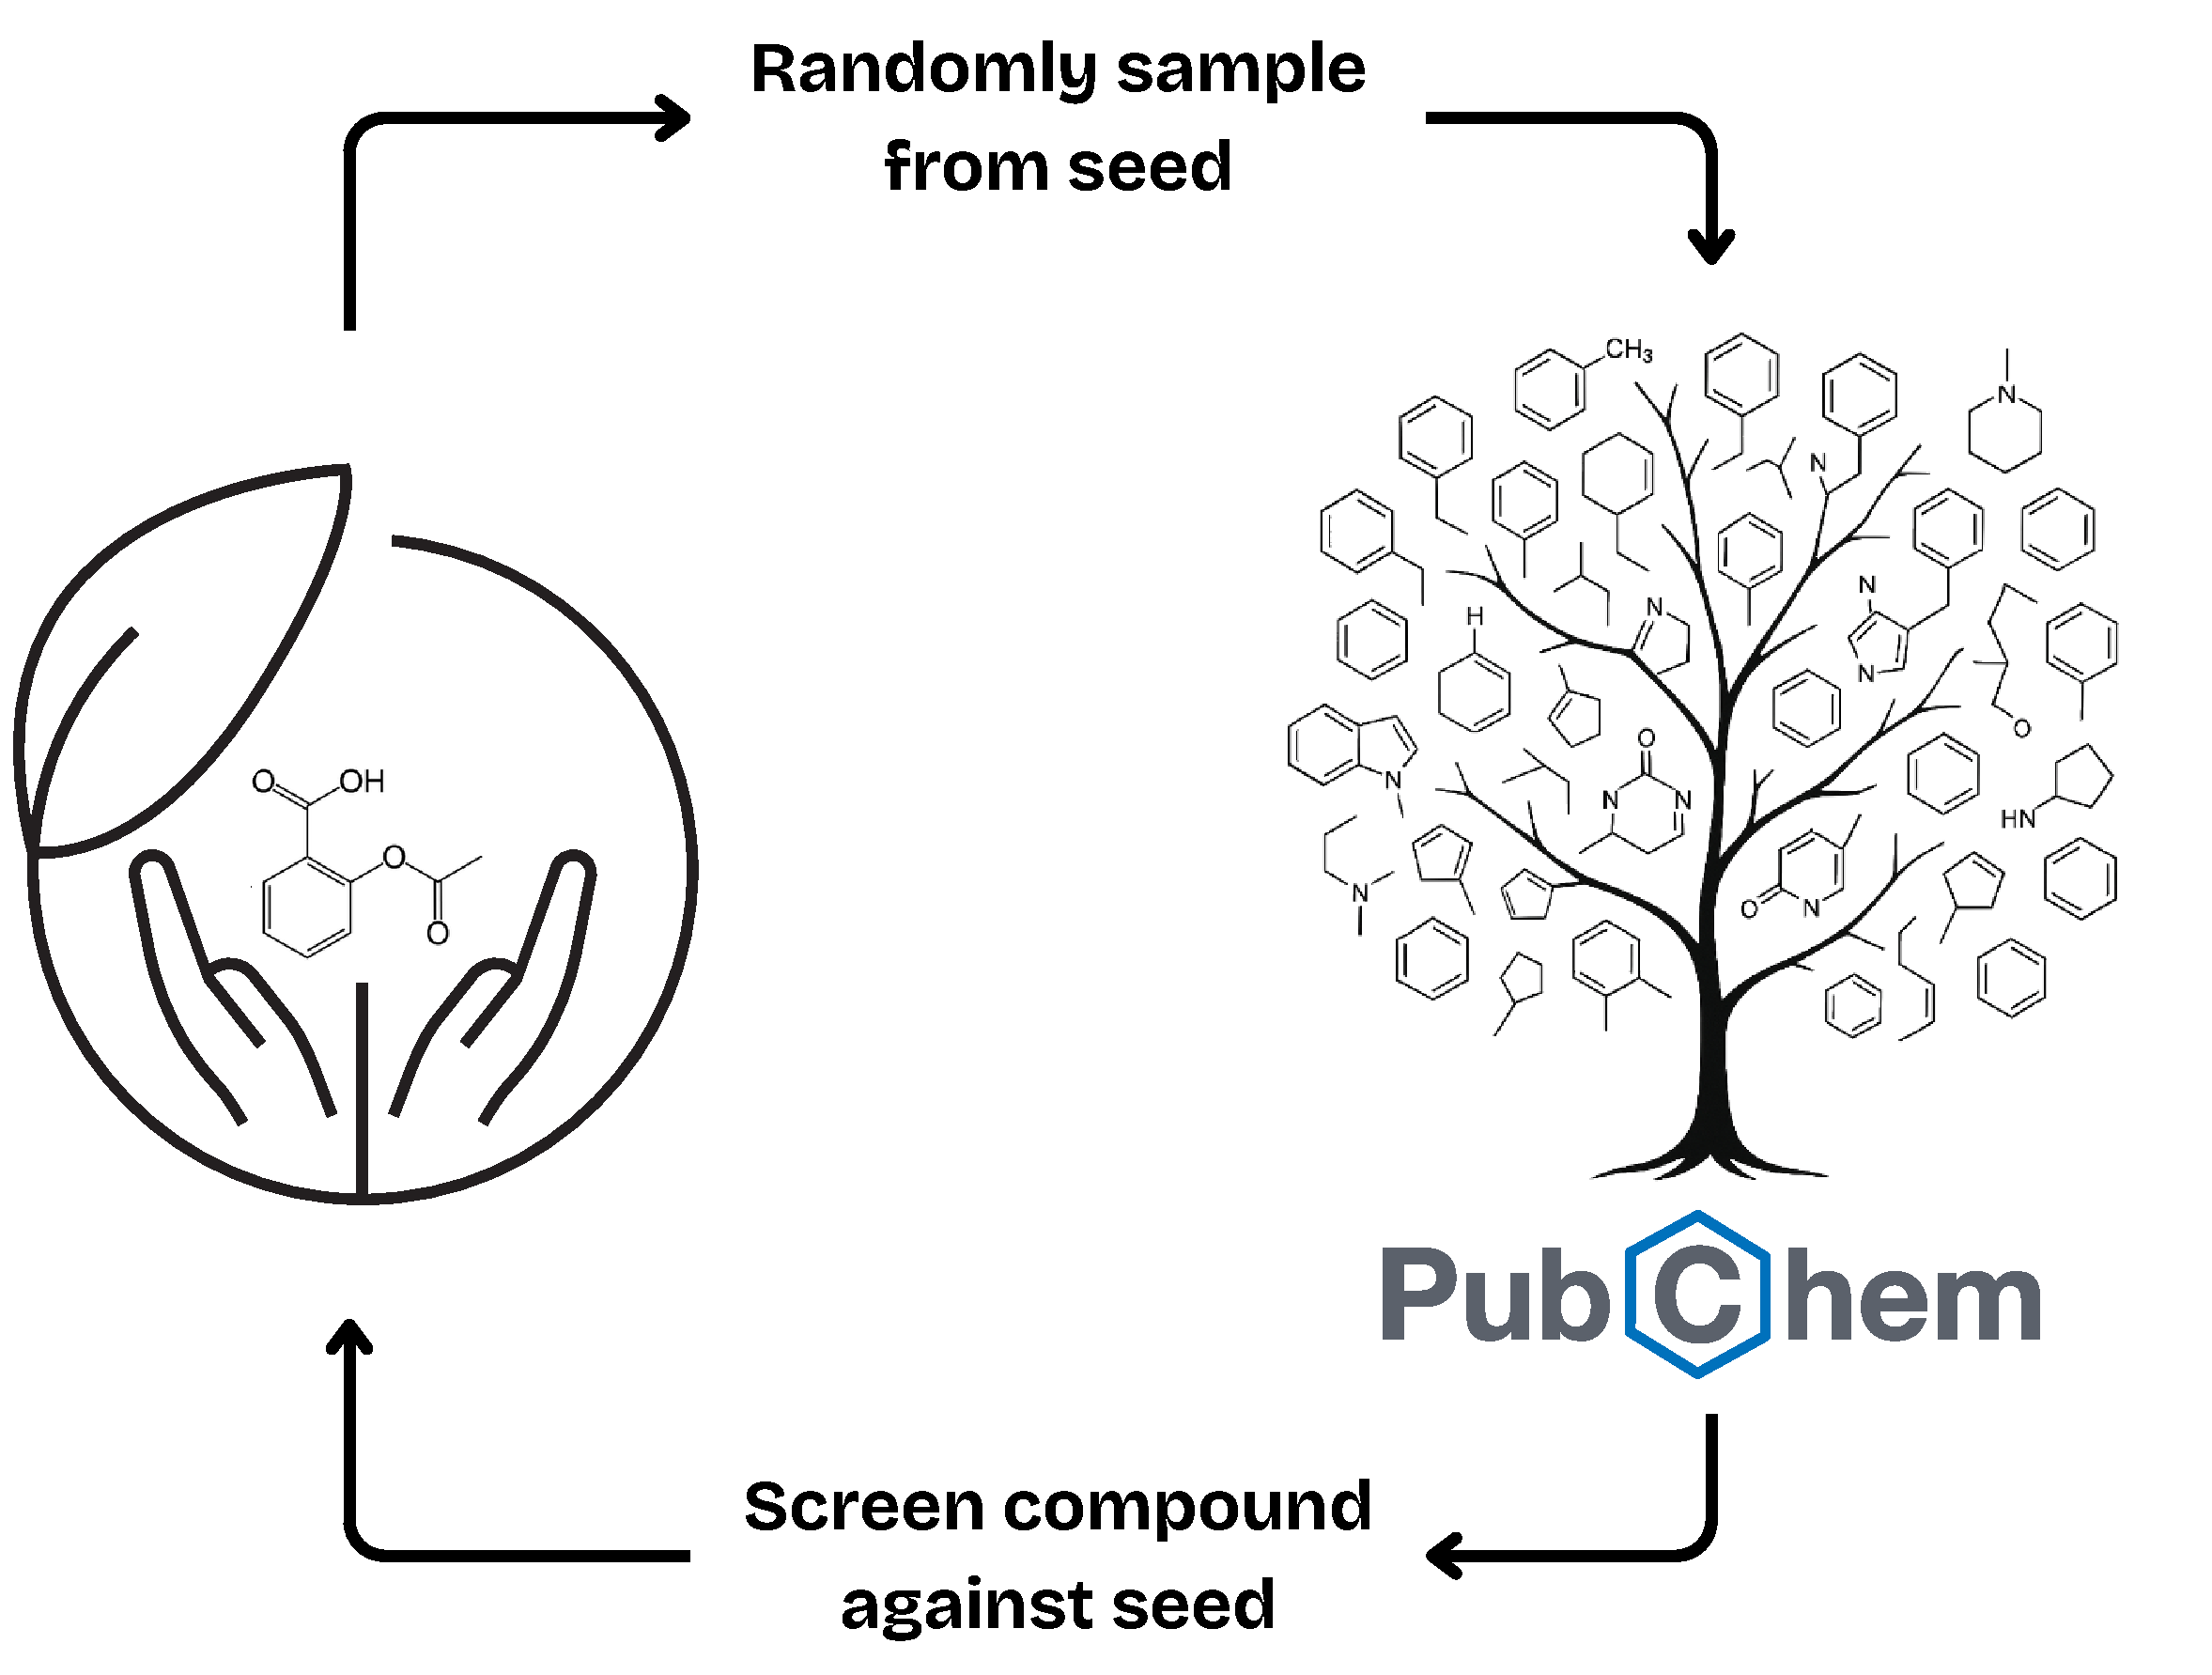
\includegraphics[width=\linewidth]{Figures/TG80.pdf}
%   \caption{Construction of TG80 from an initial seed using the PubChem database.}
%   \label{fig:dataset_construction}
% \end{wrapfigure}
Accepted candidates had an ECFP-4 Tanimoto distance between 0.875 and 0.925 (i.e., similarity between 0.075 and 0.125) to at least one seed molecule, and no more than 0.2 Tanimoto similarity to previously accepted molecules, alongside other criteria detailed in \Cref{sec:tg80_algorithm} \cite{greg_landrum_rdkitrdkit_2025, rogers_extended-connectivity_2010, rogers_computer_1960}. These thresholds follow common practice in the literature, balancing diversity while avoiding collapse into overly narrow chemical subspaces \cite{matter_selecting_1997, menke_natural_2021, eastman_spice_2023, harper_research_2004, zhang_activity_2023}.

We generate all trajectories using ORCA V6.01 \cite{neese_software_2022} with the PBE functional \cite{perdew_generalized_1996}, def2-SVP basis set \cite{weigend_balanced_2005}, \(\Delta\)4 dispersion corrections \cite{caldeweyher_generally_2019, caldeweyher_extension_2020, wittmann_extension_2024} at one femtosecond resolution, 300K temperature, in vacuum. This resembles an enhanced RMD17, with more modern dispersion corrections to improve stability and allow for a larger step size \cite{christensen_role_2020}. As a result, TG80 exhibits \textit{more diverse dynamics} and \textit{improved numerical stability}, with no compound exceeding 5~\AA{}\(^2\) position variance in \Cref{fig:numerical_stability}\footnote{Simulations ran on 32 AMD EPYC 7543 cores with 256\,GB RAM per molecule, totalling 806{,}400 CPU-hours (quoted market cost USD~150\;000).}.
\vspace{-0.3em}
\section{Experiment Results}
\vspace{-0.5em}
\textbf{Metrics.}
We use \textit{State-to-trajectory}  ($\operatorname{S2T}$) and \textit{state-to-state} ($\operatorname{S2S}$) error to evaluate \gls{atoms}  \cite{xu_equivariant_2024}. Specifically,  $\operatorname{S2T} = \frac{1}{P}\sum_{p=1}^P\|\hat{\mathbf{x}}_p - \mathbf{x}_p\|_2^2$, measures the average discrepancy between the predicted \(\hat{\mathbf{x}}\) and ground-truth positions \(\mathbf{x}\) across entire trajectories, while  $\operatorname{S2S} = \|\hat{\mathbf{x}}_P - \mathbf{x}_P\|_2^2$, quantifies the error at the final predicted timestep.
% \begin{align}
%     \operatorname{S2T} = \frac{1}{P}\sum\limits_{p=1}^P\|\mathbf{x}_p - \mathbf{x}^\dagger_p\|_2^2, \qquad \operatorname{S2S} = \|\mathbf{x}_P - \mathbf{x}^\dagger_P\|_2^2.
% \end{align}



\textbf{Baselines.} For comparison, we include a range of classic to state-of-the-art baselines, including Radial Field (RF) \cite{kohler_equivariant_2019}, Tensor Field Networks (TFN) \citep{thomas_tensor_2018}, SE(3) Transformer (SE(3)-Tr.) \citep{fuchs_se3-transformers_2020}, E(n) equivariant graph neural networks (EGNN) \citep{garcia_satorras_en_2021}, MACE \cite{batatia_mace_2023}, and \gls{egno} \citep{xu_equivariant_2024}. We note that MACE is pretrained on the authors’ own dataset, so this is not a strictly like-for-like comparison. Our EGNN baselines are {EGNN-R}ollout (EGNN-R), which predicts timesteps autoregressively, and {EGNN-S}equential (EGNN-S), which uses the output of each \gls{gnn} as the prediction of a given frame. 
% We implement an improved \gls{egno} baseline and set \gls{atoms} hidden size to 128 with five transformer blocks. 
We set all baseline hyperparameters following previous works \cite{xu_equivariant_2024, xu_geodiff_2022, shi_learning_2021} and tune \gls{atoms} and \gls{egno} hyperparameters as in \Cref{tab:atom_hparams} and \Cref{tab:egno_hparams}. 


\textbf{Training setups.}
For training of \gls{atoms} and \gls{egno}, we consider two temporal discretization strategies in selecting the timestamps $t_p =t+\sum_{r=1}^{p}\Delta t_r$: (1) \textit{Uniform discretization} selects $t_p = t + p/P \Delta T$ and (2) \textit{Tail discretization} selects $t_p = t + \overline{\Delta} + p/P (\Delta T - \overline{\Delta})$ for a lag $\overline{\Delta} \in [0, \Delta T]$. In the main paper, we present experiment results with {uniform discretization} and include the results with tail discretization in Appendix \ref{app:further_experiment}.  We perform early stopping on the lowest S2S validation loss checkpoint and report results as mean \(\pm 2 \sigma\) over \textit{three training runs}. All experiments are run on an NVIDIA\textsuperscript{\textregistered} RTX 5080 with wall-clock time and FLOP utilization detailed in \Cref{tab:md17_compute_cost}.


\subsection{Single-task Learning}
\label{sec:singletask_learning}
We benchmark on the MD17, RMD17, {and MD22} \gls{dft} \gls{md} trajectory datasets \cite{chmiela_machine_2017, christensen_role_2020, chmiela_accurate_2023}. We partition the trajectories into train/validation/test splits of sizes 500/2000/2000, set \(\Delta T = 3000\) fs and \(P = 8\) following \cite{xu_equivariant_2024}, and train for 1000 epochs. For the performance on MD17 ( \Cref{tab:md17_results}), we directly quote the results from \cite{xu_equivariant_2024} except for EGNO. 
We design \gls{atoms} to have six transformer blocks with a hidden size of 256 (seven blocks on MD22 stachyose; \Cref{appx:my_hyperparams}).
% \AHcomment{We present the results by taking average and standard deviation of \AHcomment{xxx} independent runs.}

\textbf{MD17 and RMD17.} 
As shown in \Cref{tab:md17_results}, \gls{atoms} compares favorably with \gls{sota} baselines on MD17 dataset, 
% outperforms strong \gls{sota} baselines on nearly all molecules, 
reducing the S2S and S2T \gls{mse} of \gls{egno} by 22.72\% and 22.90\% on average\footnote{We exclude benzene from the table due to the previously discussed high numerical noise.}. In \Cref{tab:rmd17_results} (Appendix~\ref{sect:rmd17}), we benchmark \gls{atoms} on RMD17, where it reduces the S2S and S2T \gls{mse} of \gls{egno} by 19.35\% and 19.89\% on average.
% The largest S2S gains occur on \emph{toluene} (54.21\%) and \emph{Aspirin} (29.21). 
% Atom achieves parity on RMD17: in \Cref{tab:rmd17_results} (Appendix~\ref{sect:rmd17}), likely as a result of the lower-noise baseline reducing the effect of label noise.

% From Table \ref{tab:md17_results}, \gls{atoms} consistently outperforms existing \gls{sota} baselines on almost all molecules, substantially improving S2S \gls{mse} by an average of 14.96\% and S2T \gls{mse} by 14.00\%. Our model achieves the largest reductions in S2S \gls{mse} for toluene (57.07\%) and Aspirin (33.73\%). 
% \AHcomment{but exhibits a performance regression on malonaldehyde of 19.57\%. We suspect that this is due to implicit hydrogen representation inadequately modeling electron delocalization effects. However, experiments in  \Cref{tab:explicit_hydrogens} seem inconclusive. (revisit)}
% \textbf{RMD17.} 
% In \Cref{tab:rmd17_results} (Appendix \ref{sect:rmd17}) we also compare \gls{atoms} and \gls{egno} on RMD17 dataset and observe a similar leading performance consistently. 

% \AHcomment{
% show that \gls{atoms} also achieves leading results on the RMD17 dataset with a mean S2T improvement of 12\%, surpassing the previous \gls{sota} in all but one case. The largest gain of 23.24\% occurs for naphthalene, and \gls{atoms} sees fewer performance regressions compared to \gls{egno} than on MD17. The more modest mean improvement relative to \gls{egno} likely reflects the lower noise level in RMD17, reducing the effect of label-noise regularization. As such, we claim label noise should only be included when the underlying ground truth trajectories contain numerical errors.
% }

\begin{wrapfigure}{r}{0.25\textwidth}
    \vspace{-1em}
    \centering
    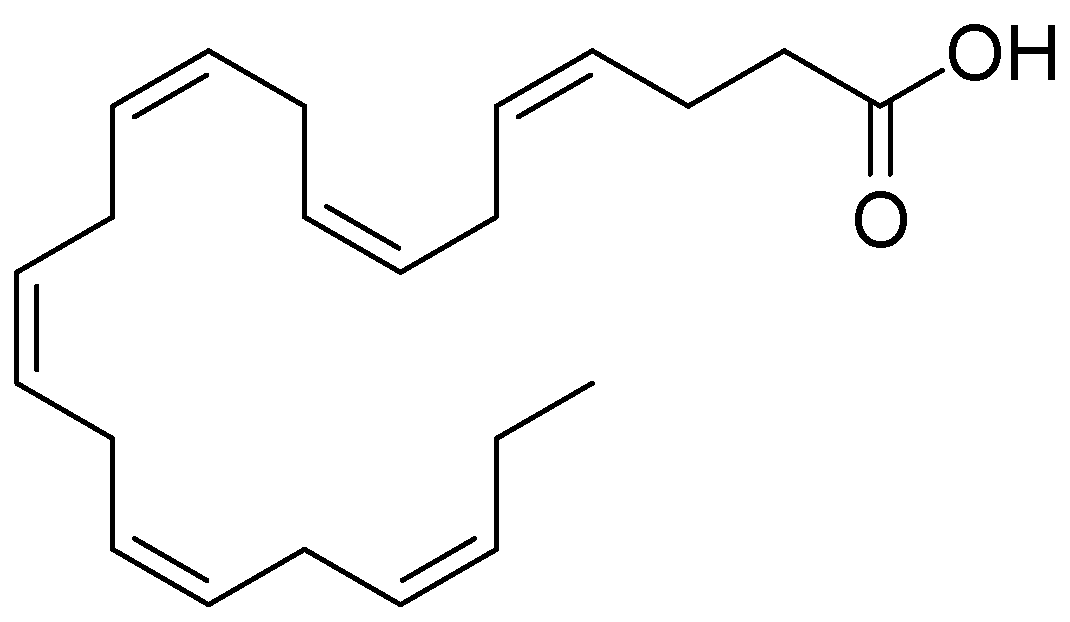
\includegraphics[width=\linewidth]{Figures/dataset/Docosahexaenoic_acid_structure.pdf}
    \caption{Docosahexaenoic acid (DHA)}
    \label{fig:dha}
    \vspace{-1em}
\end{wrapfigure}
\textbf{MD22.} To evaluate performance on larger molecules, we consider Ac-Ala3-NHMe (20 heavy atoms), docosahexaenoic acid (DHA with 24 heavy atoms), and stachyose (45 heavy atoms) from the MD22 dataset \cite{chmiela_accurate_2023}. \gls{atoms} remains competitive on these systems; whereas \gls{egno} fails to converge (\Cref{tab:md22_results}). We attribute this discrepancy to differing inductive biases: \Glspl{gnn} such as \gls{egno} restrict message passing to a predefined bond or radius graph and can therefore under-represent long-range, non-bonded steric and electrostatic interactions that dominate the behavior of large, sparsely connected molecules \cite{alon_bottleneck_2021,kosmala_ewald-based_2023}. This explains the poor performance of \gls{egno} on MD22, which contains prototypically sparse molecules such as DHA, shown in \Cref{fig:dha} \cite{nv_polyunsaturated_2003}. {We further disentangle the role of connectivity from the use of attention by training a variant, \gls{atoms}-GATv2, in which our heterogeneous temporal attention is replaced by \gls{gatv2} layers \cite{brody_how_2022} operating on the same bond/radius graph as \gls{egno}. \gls{atoms}-\gls{gatv2} still substantially underperforms the full \gls{atoms} model, indicating that the performance gains stem from the fully connected point-cloud interaction pattern rather than from attention alone.}



% \begin{table}[t]
% %— Top: Full‐width big table —
% \centering
% \caption{MSE (\(\times 10^{-2}\)) on MD17. Upper part: S2S \gls{mse}. Lower part: S2T \gls{mse}.}
% \label{tab:md17_results}
% \resizebox{\linewidth}{!}{%
%   \begin{tabular}{lcccccccc }
%     \toprule
%     & \textbf{Aspirin} & \textbf{Benzene} & \textbf{Ethanol} & \textbf{Malonaldehyde} & \textbf{Naphthalene} & \textbf{Salicylic} & \textbf{Toluene} & \textbf{Uracil} 
%     % & Mean \% 
%     \\
%     \midrule
%     RF & \(10.94{\scriptstyle \pm0.02}\) & \(103.72{\scriptstyle \pm2.58}\) & \(4.64{\scriptstyle \pm0.02}\) & \(13.93{\scriptstyle \pm0.06}\) & \(0.50{\scriptstyle \pm0.02}\) & \(1.23{\scriptstyle \pm0.04}\) & \(10.93{\scriptstyle \pm0.08}\) & \(0.64{\scriptstyle \pm0.02}\) \\
%     TFN  & \(12.37{\scriptstyle \pm0.36}\) & \(58.48{\scriptstyle \pm3.96}\)  & \(4.81{\scriptstyle \pm0.08}\) & \(13.62{\scriptstyle \pm0.16}\) & \(0.49{\scriptstyle \pm0.02}\) & \(1.03{\scriptstyle \pm0.04}\) & \(10.89{\scriptstyle \pm0.02}\) & \(0.84{\scriptstyle \pm0.04}\) \\
%     SE(3)-Tr. & \(11.12{\scriptstyle \pm0.12}\) & \(68.11{\scriptstyle \pm1.34}\) & \(4.74{\scriptstyle \pm0.02}\) & \(13.89{\scriptstyle \pm0.04}\) & \(0.52{\scriptstyle \pm0.02}\) & \(1.13{\scriptstyle \pm0.04}\) & \(10.88{\scriptstyle \pm0.12}\) & \(0.79{\scriptstyle \pm0.04}\) \\
%     EGNN & \(14.41{\scriptstyle \pm0.30}\) & \(62.40{\scriptstyle \pm1.06}\) & \(4.64{\scriptstyle \pm0.04}\) & \(13.64{\scriptstyle \pm0.02}\) & \(0.47{\scriptstyle \pm0.04}\) & \(1.02{\scriptstyle \pm0.04}\) & \(11.78{\scriptstyle \pm0.14}\) & \(0.64{\scriptstyle \pm0.02}\) \\
%     EGNN-R & \(14.51{\scriptstyle \pm0.38}\) & \(62.61{\scriptstyle \pm1.50}\) & \(4.94{\scriptstyle \pm0.08}\) & \(17.25{\scriptstyle \pm0.10}\) & \(0.82{\scriptstyle \pm0.04}\) & \(1.35{\scriptstyle \pm0.04}\) & \(11.59{\scriptstyle \pm0.08}\) & \(1.11{\scriptstyle \pm0.04}\) \\
%     EGNN-S & \(9.50{\scriptstyle \pm0.20}\) & \(66.45{\scriptstyle \pm1.78}\)  & \(4.63{\scriptstyle \pm0.02}\) & \(12.88{\scriptstyle \pm0.02}\) & \(0.45{\scriptstyle \pm0.02}\) & \(1.00{\scriptstyle \pm0.04}\) & \(10.78{\scriptstyle \pm0.10}\) & \(0.60{\scriptstyle \pm0.02}\) \\
%     \gls{egno} & \(9.64{\scriptstyle \pm0.15}\) & \(40.75{\scriptstyle \pm3.64}\) & \(4.57{\scriptstyle \pm0.01}\) & \(\mathbf{12.92}{\scriptstyle \pm0.00}\) & \(0.39{\scriptstyle \pm0.00}\) & \(0.89{\scriptstyle \pm0.01}\) & \(11.00{\scriptstyle \pm0.00}\) & \(0.58{\scriptstyle \pm0.02}\) &  \\
%     \gls{atoms} & \(\mathbf{6.46}{\scriptstyle \pm0.09}\) & \(\mathbf{38.39}{\scriptstyle \pm2.38}\) & \(\mathbf{3.70}{\scriptstyle \pm0.07}\) & \(15.45{\scriptstyle \pm0.97}\) & \(\mathbf{0.39}{\scriptstyle \pm0.00}\) & \(\mathbf{0.83}{\scriptstyle \pm0.00}\) & \(\mathbf{4.72}{\scriptstyle \pm0.03}\) & \(\mathbf{0.54}{\scriptstyle \pm0.01}\) &  \\
%     \midrule
%     \rowcolor{gray!20} Gap  & \(+33.03\%\) & \(+5.80\%\) & \(+19.09\%\) & \(-19.57\%\) & \(+1.84\%\) & \(6.57\%\) & \(57.07\%\) & \(7.85\%\) 
%     % & \(13.96\%\) 
%     \\
%     \midrule
%     EGNN-R & \(12.07{\scriptstyle \pm0.22}\) & \(23.73{\scriptstyle \pm0.60}\) & \(3.44{\scriptstyle \pm0.34}\) & \(13.38{\scriptstyle \pm0.06}\) & \(0.63{\scriptstyle \pm0.02}\) & \(1.15{\scriptstyle \pm0.04}\) & \(5.04{\scriptstyle \pm0.04}\) & \(0.89{\scriptstyle \pm0.02}\) \\
%     EGNN-S & \(9.49{\scriptstyle \pm0.24}\) & \(29.99{\scriptstyle \pm1.30}\) & \(3.29{\scriptstyle \pm0.02}\) & \(11.21{\scriptstyle \pm0.02}\) & \(0.43{\scriptstyle \pm0.02}\) & \(1.36{\scriptstyle \pm0.04}\) & \(4.85{\scriptstyle \pm0.08}\) & \(0.68{\scriptstyle \pm0.02}\) \\
%     \gls{egno} & \(9.64{\scriptstyle \pm0.15}\) & \(40.73{\scriptstyle \pm3.67}\) & \(4.57{\scriptstyle \pm0.01}\) & \(\mathbf{12.92}{\scriptstyle \pm0.00}\) & \(0.39{\scriptstyle \pm0.00}\) & \(0.90{\scriptstyle \pm0.01}\) & \(10.99{\scriptstyle \pm0.00}\) & \(0.58{\scriptstyle \pm0.02}\) &  \\
%     \gls{atoms} & \(\mathbf{6.46}{\scriptstyle \pm0.08}\) & \(\mathbf{38.39}{\scriptstyle \pm2.39}\) & \(\mathbf{3.70}{\scriptstyle \pm0.07}\) & \(15.45{\scriptstyle \pm0.97}\) & \(\mathbf{0.38}{\scriptstyle \pm0.00}\) & \(\mathbf{0.83}{\scriptstyle \pm0.00}\) & \(\mathbf{4.72}{\scriptstyle \pm0.02}\) & \(\mathbf{0.54}{\scriptstyle \pm0.01}\) &  \\
%     \midrule
%     \rowcolor{gray!20} Gap & \(32.96\%\) & \(5.74\%\) & \(19.03\%\) & \(-19.59\%\) & \(2.06\%\) & \(6.90\%\) & \(57.09\%\) & \(7.84\%\) 
%     % & \(14.00\%\)
%     \\
%     \bottomrule
%   \end{tabular}
% }
% \end{table}

% \begin{table}[t]
% %— Top: Full‐width big table —
% \centering
% \caption{Single-task MSE (\(\times 10^{-2}\)) on MD17. Upper part: S2S \gls{mse}. Lower part: S2T \gls{mse}. \AHcomment{check the numbers}}
% \label{tab:md17_results}
% \resizebox{\linewidth}{!}{%
%   \begin{tabular}{lcccccccc }
%     \toprule
%     & \textbf{Aspirin} & \textbf{Benzene} & \textbf{Ethanol} & \textbf{Malonaldehyde} & \textbf{Naphthalene} & \textbf{Salicylic} & \textbf{Toluene} & \textbf{Uracil} 
%     % & Mean \% 
%     \\
%     \midrule
%     RF & \(10.94{\scriptstyle \pm0.02}\) & \(103.72{\scriptstyle \pm2.58}\) & \(4.64{\scriptstyle \pm0.02}\) & \(13.93{\scriptstyle \pm0.06}\) & \(0.50{\scriptstyle \pm0.02}\) & \(1.23{\scriptstyle \pm0.04}\) & \(10.93{\scriptstyle \pm0.08}\) & \(0.64{\scriptstyle \pm0.02}\) \\
%     TFN  & \(12.37{\scriptstyle \pm0.36}\) & \(58.48{\scriptstyle \pm3.96}\)  & \(4.81{\scriptstyle \pm0.08}\) & \(13.62{\scriptstyle \pm0.16}\) & \(0.49{\scriptstyle \pm0.02}\) & \(1.03{\scriptstyle \pm0.04}\) & \(10.89{\scriptstyle \pm0.02}\) & \(0.84{\scriptstyle \pm0.04}\) \\
%     SE(3)-Tr. & \(11.12{\scriptstyle \pm0.12}\) & \(68.11{\scriptstyle \pm1.34}\) & \(4.74{\scriptstyle \pm0.02}\) & \(13.89{\scriptstyle \pm0.04}\) & \(0.52{\scriptstyle \pm0.02}\) & \(1.13{\scriptstyle \pm0.04}\) & \(10.88{\scriptstyle \pm0.12}\) & \(0.79{\scriptstyle \pm0.04}\) \\
%     EGNN & \(14.41{\scriptstyle \pm0.30}\) & \(62.40{\scriptstyle \pm1.06}\) & \(4.64{\scriptstyle \pm0.04}\) & \(13.64{\scriptstyle \pm0.02}\) & \(0.47{\scriptstyle \pm0.04}\) & \(1.02{\scriptstyle \pm0.04}\) & \(11.78{\scriptstyle \pm0.14}\) & \(0.64{\scriptstyle \pm0.02}\) \\
%     EGNN-R & \(14.51{\scriptstyle \pm0.38}\) & \(62.61{\scriptstyle \pm1.50}\) & \(4.94{\scriptstyle \pm0.08}\) & \(17.25{\scriptstyle \pm0.10}\) & \(0.82{\scriptstyle \pm0.04}\) & \(1.35{\scriptstyle \pm0.04}\) & \(11.59{\scriptstyle \pm0.08}\) & \(1.11{\scriptstyle \pm0.04}\) \\
%     EGNN-S & \(9.50{\scriptstyle \pm0.20}\) & \(66.45{\scriptstyle \pm1.78}\)  & \(4.63{\scriptstyle \pm0.02}\) & \(12.88{\scriptstyle \pm0.02}\) & \(0.45{\scriptstyle \pm0.02}\) & \(1.00{\scriptstyle \pm0.04}\) & \(10.78{\scriptstyle \pm0.10}\) & \(0.60{\scriptstyle \pm0.02}\) \\
%     \gls{egno} & \(9.64{\scriptstyle \pm0.15}\) & \(40.75{\scriptstyle \pm3.64}\) & \(4.57{\scriptstyle \pm0.01}\) & \(\mathbf{12.92}{\scriptstyle \pm0.00}\) & \(0.39{\scriptstyle \pm0.00}\) & \(0.89{\scriptstyle \pm0.01}\) & \(11.00{\scriptstyle \pm0.00}\) & \(0.58{\scriptstyle \pm0.02}\)  \\
%     \textbf{ATOM} & \(\mathbf{6.46}{\scriptstyle \pm0.09}\) & \(\mathbf{38.39}{\scriptstyle \pm2.38}\) & \(\mathbf{3.70}{\scriptstyle \pm0.07}\) & \(15.45{\scriptstyle \pm0.97}\) & \(\mathbf{0.39}{\scriptstyle \pm0.00}\) & \(\mathbf{0.83}{\scriptstyle \pm0.00}\) & \(\mathbf{4.72}{\scriptstyle \pm0.03}\) & \(\mathbf{0.54}{\scriptstyle \pm0.01}\)   \\
%     \midrule
%     \rowcolor{gray!20} Gap  & \(+33.03\%\) & \(+5.80\%\) & \(+19.09\%\) & \(-19.57\%\) & \(+1.84\%\) & \(+6.57\%\) & \(+57.07\%\) & \(+7.85\%\) 
%     % & \(13.96\%\) 
%     \\
%     \midrule
%     EGNN-R & \(12.07{\scriptstyle \pm0.22}\) & \(23.73{\scriptstyle \pm0.60}\) & \(3.44{\scriptstyle \pm0.34}\) & \(13.38{\scriptstyle \pm0.06}\) & \(0.63{\scriptstyle \pm0.02}\) & \(1.15{\scriptstyle \pm0.04}\) & \(5.04{\scriptstyle \pm0.04}\) & \(0.89{\scriptstyle \pm0.02}\) \\
%     EGNN-S & \(9.49{\scriptstyle \pm0.24}\) & \(29.99{\scriptstyle \pm1.30}\) & \(3.29{\scriptstyle \pm0.02}\) & \(11.21{\scriptstyle \pm0.02}\) & \(0.43{\scriptstyle \pm0.02}\) & \(1.36{\scriptstyle \pm0.04}\) & \(4.85{\scriptstyle \pm0.08}\) & \(0.68{\scriptstyle \pm0.02}\) \\
%     \gls{egno} & \(8.51{\scriptstyle \pm0.03}\) & \(\mathbf{23.61}{\scriptstyle \pm0.03}\) & \(\mathbf{40.32}{\scriptstyle \pm0.08}\) & \(1.42{\scriptstyle \pm0.00}\) & \(\mathbf{28.01}{\scriptstyle \pm0.02}\) & \(1.07{\scriptstyle \pm0.01}\) & \(\mathbf{28.23}{\scriptstyle \pm0.00}\) & \(0.87{\scriptstyle \pm0.00}\) \\
%     \gls{atoms} & \(\mathbf{8.38}{\scriptstyle \pm0.05}\) & \(23.90{\scriptstyle \pm0.15}\) & \(40.67{\scriptstyle \pm0.17}\) & \(\mathbf{1.36}{\scriptstyle \pm0.00}\) & \(56.93{\scriptstyle \pm20.78}\) & \(\mathbf{1.04}{\scriptstyle \pm0.00}\) & \(28.58{\scriptstyle \pm0.05}\) & \(\mathbf{0.85}{\scriptstyle \pm0.00}\) \\
%     \midrule
%     \rowcolor{gray!20} Gap & \(+32.96\%\) & \(+5.74\%\) & \(+19.03\%\) & \(-19.59\%\) & \(+2.06\%\) & \(+6.90\%\) & \(+57.09\%\) & \(+7.84\%\) 
%     % & \(14.00\%\)
%     \\
%     \bottomrule
%   \end{tabular}
% }
% \end{table}

\begin{table}[t]
%— Top: Full‐width big table —
\centering
\caption{Single-task MSE (\(\times 10^{-2}\)) on MD17. Upper part: S2S \gls{mse}. Lower part: S2T \gls{mse}.}
\label{tab:md17_results}
\resizebox{\linewidth}{!}{%
    \begin{tabular}{lccccccc}
        \toprule
         & Aspirin & Ethanol & Malonaldehyde & Naphthalene & Salicylic & Toluene & Uracil \\
        \midrule
        RF & \(10.94{\scriptstyle \pm0.02}\) & \(4.64{\scriptstyle \pm0.02}\) & \(13.93{\scriptstyle \pm0.06}\) & \(0.50{\scriptstyle \pm0.02}\) & \(1.23{\scriptstyle \pm0.04}\) & \(10.93{\scriptstyle \pm0.08}\) & \(0.64{\scriptstyle \pm0.02}\) \\
        TFN  & \(12.37{\scriptstyle \pm0.36}\) & \(4.81{\scriptstyle \pm0.08}\) & \(13.62{\scriptstyle \pm0.16}\) & \(0.49{\scriptstyle \pm0.02}\) & \(1.03{\scriptstyle \pm0.04}\) & \(10.89{\scriptstyle \pm0.02}\) & \(0.84{\scriptstyle \pm0.04}\) \\
        SE(3)-Tr. & \(11.12{\scriptstyle \pm0.12}\) & \(4.74{\scriptstyle \pm0.02}\) & \(13.89{\scriptstyle \pm0.04}\) & \(0.52{\scriptstyle \pm0.02}\) & \(1.13{\scriptstyle \pm0.04}\) & \(10.88{\scriptstyle \pm0.12}\) & \(0.79{\scriptstyle \pm0.04}\) \\
        EGNN & \(14.41{\scriptstyle \pm0.30}\) & \(4.64{\scriptstyle \pm0.04}\) & \(13.64{\scriptstyle \pm0.02}\) & \(0.47{\scriptstyle \pm0.04}\) & \(1.02{\scriptstyle \pm0.04}\) & \(11.78{\scriptstyle \pm0.14}\) & \(0.64{\scriptstyle \pm0.02}\) \\
        EGNN-R & \(9.96{\scriptstyle \pm0.14}\) & \(4.61{\scriptstyle \pm0.01}\) & \(\mathbf{13.04}{\scriptstyle \pm0.03}\) & \(0.44{\scriptstyle \pm0.05}\) & \(0.96{\scriptstyle \pm0.01}\) & \(10.19{\scriptstyle \pm0.15}\) & \(1.11{\scriptstyle \pm0.04}\) \\
        EGNN-S & \(10.25{\scriptstyle \pm0.09}\) & \(4.61{\scriptstyle \pm0.01}\) & \(13.06{\scriptstyle \pm0.01}\) & \(0.53{\scriptstyle \pm0.01}\) & \(1.06{\scriptstyle \pm0.05}\) & \(10.83{\scriptstyle \pm0.09}\) & \(0.62{\scriptstyle \pm0.01}\) \\
        \gls{egno} & \(10.05{\scriptstyle \pm0.01}\) & \(4.67{\scriptstyle \pm0.04}\) & \(13.21{\scriptstyle \pm0.06}\) & \(0.50{\scriptstyle \pm0.00}\) & \(0.94{\scriptstyle \pm0.00}\) & \(11.04{\scriptstyle \pm0.37}\) & \(0.63{\scriptstyle \pm0.00}\) \\
          MACE & \(6.95\pm\scriptstyle{0.00}\) & \(2.06\pm\scriptstyle{0.00}\) & \(17.99\pm\scriptstyle{0.26}\) & \(0.72\pm\scriptstyle{0.00}\) & \(1.05\pm\scriptstyle{0.00}\) & \(6.44\pm\scriptstyle{0.00}\) & \(0.75\pm\scriptstyle{0.00}\) \\  
        \textbf{\gls{atoms}} & \(\mathbf{6.60}{\scriptstyle \pm0.03}\) & \(\mathbf{3.27}{\scriptstyle \pm0.03}\) & \(13.77{\scriptstyle \pm0.16}\) & \(\mathbf{0.38}{\scriptstyle \pm0.00}\) & \(\mathbf{0.82}{\scriptstyle \pm0.00}\) & \(\mathbf{5.65}{\scriptstyle \pm0.05}\) & \(\mathbf{0.55}{\scriptstyle \pm0.00}\) \\
        % \midrule
        % \rowcolor{gray!20} Gap & \(+29.29\%\) & \(+23.07\%\) & \(-13.93\%\) & \(-27.20\%\) & \(+1.05\%\) & \(+54.21\%\) & \(-7.78\%\) \\
        \midrule
        EGNN-R & \(7.35{\scriptstyle \pm0.19}\) & \(3.21{\scriptstyle \pm0.00}\) & \(\mathbf{10.75}{\scriptstyle \pm0.04}\) & \(\mathbf{0.34}{\scriptstyle \pm0.06}\) & \(1.09{\scriptstyle \pm0.12}\) & \(4.53{\scriptstyle \pm0.08}\) & \(0.89{\scriptstyle \pm0.02}\) \\
        EGNN-S & \(9.01{\scriptstyle \pm0.34}\) & \(3.21{\scriptstyle \pm0.00}\) & \(11.20{\scriptstyle \pm0.03}\) & \(0.42{\scriptstyle \pm0.01}\) & \(1.41{\scriptstyle \pm0.00}\) & \(4.86{\scriptstyle \pm0.04}\) & \(0.65{\scriptstyle \pm0.01}\) \\
        \gls{egno} & \(7.92{\scriptstyle \pm0.04}\) & \(3.25{\scriptstyle \pm0.01}\) & \(11.44{\scriptstyle \pm0.03}\) & \(0.42{\scriptstyle \pm0.00}\) & \(0.95{\scriptstyle \pm0.02}\) & \(4.87{\scriptstyle \pm0.16}\) & \(0.61{\scriptstyle \pm0.00}\) \\
         MACE & \(5.06\pm\scriptstyle{0.00}\) & \(2.84\pm\scriptstyle{0.00}\) & \(16.09\pm\scriptstyle{0.03}\) & \(0.57\pm\scriptstyle{0.00}\) & \(0.55\pm\scriptstyle{0.00}\) & \(3.26\pm\scriptstyle{0.00}\) & \(1.08\pm\scriptstyle{0.00}\) \\
        \textbf{\gls{atoms}} & \(\mathbf{5.27}{\scriptstyle \pm0.02}\) & \(\mathbf{2.39}{\scriptstyle \pm0.02}\) & \(11.76{\scriptstyle \pm0.09}\) & \(0.36{\scriptstyle \pm0.00}\) & \(\mathbf{0.70}{\scriptstyle \pm0.00}\) & \(\mathbf{2.65}{\scriptstyle \pm0.01}\) & \(\mathbf{0.51}{\scriptstyle \pm0.00}\) \\
        % \midrule
        % \rowcolor{gray!20} Gap & \(+23.57\%\) & \(+18.33\%\) & \(-16.22\%\) & \(-24.11\%\) & \(+3.90\%\) & \(+49.95\%\) & \(-4.77\%\) \\
        \bottomrule
    \end{tabular}
}
\end{table}


% \vspace{-1em}


% \begin{minipage}{\textwidth}
% \paragraph{Large \(\Delta t\) MD17} Large time-horizon (\(\Delta t\)) \gls{md} simulations necessitate high-precision methods to prevent the accumulation of integration error over time \cite{liang_energy_2023}. As shown in \Cref{tab:big_delta_results}, \gls{atoms} significantly outperforms \gls{egno}~\cite{xu_equivariant_2024} for large \(\Delta t\) prediction across four molecules in MD17, reducing S2S MSE by \(77.8\%\) for aspirin and \(58.1\%\) for toluene. Similar trends hold for S2T \gls{mse}.
% \end{minipage}

\subsection{Multitask Learning on TG80}
\label{sec:multitask_learning}

We pretrain \gls{atoms} on TG80, scaling to six attention blocks with a hidden size of 256. We select stochastic horizons \(\Delta T \sim \operatorname{LogUnif}(8 \text{ fs}, 24\,000 \text{ fs})\) and use a five-fold, cluster-based cross-validation. Specifically, we compute ECFP-4 fingerprints \cite{rogers_extended-connectivity_2010}, embed them using UMAP \cite{mcinnes_umap_2018}, and apply agglomerative clustering \cite{ward_hierarchical_1963} to partition compounds into ten disjoint clusters. The folds are then formed by holding out clusters, ensuring that the train/validation/test sets occupy distinct regions of chemical space. This cluster-wise protocol minimizes leakage and more closely reflects the prospective scientific setting in which models must generalize to unseen molecules. Cluster-based approaches present more challenging generalization problems than random splits or common chemical-scaffold-based splits \cite{guo_scaffold_2024}. In Appendix \ref{sect:random_split}, we also consider pretraining on a standard random split of molecules. 

Table \ref{tab:tg80_umap} benchmarks \gls{atoms} by assessing both \textit{in-distribution} (ID) and \textit{out-of-domain} (OOD) S2T performance. For the \textit{in-distribution} setting, we train, validate, and test on molecules from the same cluster. We observe that \gls{atoms} outperforms \gls{egno} by an average of 95.26\% in terms of S2T \gls{mse}. We then assess \textit{out-of-domain} (OOD) generalization performance by predicting the dynamics of unseen compounds drawn from disjoint clusters. Under OOD settings, \gls{atoms} reduces the S2T \gls{mse} of \gls{egno} by an average of $54.17\%$ across five cluster splits.\footnote{On Cluster 2, one of three \gls{egno} OOD seeds diverged (S2T \gls{mse} 5092.68; the other two 123.36 and 138.63). Excluding Cluster 2, the mean OOD gap is 43.55\%.} Notably, OOD \gls{atoms} beats ID \gls{egno} performance in all five folds. This striking zero-shot generalization, realized without any exposure to the test molecules, confirms that \gls{atoms} uniquely learns robust, transferable knowledge of molecular dynamics. In Appendix \ref{app:s2s_result}, we show similar outperformance in S2S prediction. In Appendix \ref{sec:model_compute_time}, we show that the significantly improved multitask performance comes with a modest overhead in training time and in inference latency.

% We show the compute costs in \Cref{tab:tg80_compute_cost}.

% \begin{table}[t]
%     \centering
%     \caption{OOD and ID \gls{mse} \((\times10^{-2})\) on TG80 across five UMAP cluster test set assignments with stochastic \(\Delta t \sim \log(\operatorname{Uniform}(8,\ 24\;000))\). Upper part: S2S \gls{mse}. Lower part: S2T \gls{mse}.}
%     \begin{tabular}{lccccc}
%         \toprule
%          & \textbf{Cluster 1} & \textbf{Cluster 2} & \textbf{Cluster 3} & \textbf{Cluster 4} & \textbf{Cluster 5} \\
%         \midrule
%         \gls{egno} OOD & \(52.90{\scriptstyle \pm0.72}\) & \(114.14{\scriptstyle \pm13.21}\) & \(149.99{\scriptstyle \pm0.34}\) & \(163.47{\scriptstyle \pm1.00}\) & \(112.36{\scriptstyle \pm1.90}\) \\
%         EGNN-S OOD & \(52.39{\scriptstyle \pm0.40}\) & \(16512.07{\scriptstyle \pm12314.09}\) & \(149.41{\scriptstyle \pm0.94}\) & \(663.54{\scriptstyle \pm865.23}\) & \(111.08{\scriptstyle \pm0.62}\) \\
%         EGNN-R OOD & \(52.08{\scriptstyle \pm0.79}\) & \(\mathbf{108.89}{\scriptstyle \pm1.60}\) & \(148.67{\scriptstyle \pm0.73}\) & \(163.27{\scriptstyle \pm0.16}\) & \(109.94{\scriptstyle \pm0.31}\) \\
%         \gls{egno} ID & \(51.98{\scriptstyle \pm0.81}\) & \(95.86{\scriptstyle \pm0.53}\) & \(142.51{\scriptstyle \pm0.58}\) & \(155.25{\scriptstyle \pm0.67}\) & \(109.25{\scriptstyle \pm0.24}\) \\
%         \gls{atoms} OOD & \(\mathbf{41.97}{\scriptstyle \pm1.24}\) & \(127.95{\scriptstyle \pm122.67}\) & \(\mathbf{74.53}{\scriptstyle \pm4.82}\) & \(\mathbf{80.95}{\scriptstyle \pm1.21}\) & \(\mathbf{58.26}{\scriptstyle \pm1.68}\) \\
%         \gls{atoms} ID & \(\mathbf{15.49}{\scriptstyle \pm1.04}\) & \(\mathbf{26.55}{\scriptstyle \pm2.13}\) & \(\mathbf{28.74}{\scriptstyle \pm2.40}\) & \(\mathbf{29.81}{\scriptstyle \pm2.72}\) & \(\mathbf{26.33}{\scriptstyle \pm1.98}\) \\
%         \midrule
%         \rowcolor{gray!20} OOD-OOD Gap & \(+20.66\%\) & \(-12.10\%\) & \(+50.31\%\) & \(+50.48\%\) & \(+48.15\%\) \\
%         \rowcolor{gray!20} OOD-ID Gap & \(-\%\) & \(-\%\) & \(-\%\) & \(-\%\) & \(-\%\) \\
%         \midrule
%         \gls{egno} OOD & \(45.95{\scriptstyle \pm0.80}\) & \(115.43{\scriptstyle \pm13.23}\) & \(151.74{\scriptstyle \pm0.57}\) & \(163.90{\scriptstyle \pm0.69}\) & \(113.68{\scriptstyle \pm2.50}\) \\
%         EGNN-S & \(45.44{\scriptstyle \pm0.57}\) & \(7386.15{\scriptstyle \pm6931.89}\) & \(152.72{\scriptstyle \pm0.83}\) & \(464.22{\scriptstyle \pm509.48}\) & \(114.30{\scriptstyle \pm0.79}\) \\
%         EGNN-R OOD & \(44.88{\scriptstyle \pm0.68}\) & \(109.62{\scriptstyle \pm1.92}\) & \(148.05{\scriptstyle \pm0.70}\) & \(161.54{\scriptstyle \pm0.68}\) & \(110.10{\scriptstyle \pm0.96}\) \\
%         \gls{egno} ID & \(44.23{\scriptstyle \pm0.68}\) & \(95.52{\scriptstyle \pm0.73}\) & \(141.16{\scriptstyle \pm0.21}\) & \(150.92{\scriptstyle \pm0.11}\) & \(107.47{\scriptstyle \pm0.36}\) \\
%         \gls{atoms} OOD & \(\mathbf{35.05}{\scriptstyle \pm0.97}\) & \(\mathbf{106.99}{\scriptstyle \pm104.64}\) & \(\mathbf{60.95}{\scriptstyle \pm4.86}\) & \(\mathbf{66.68}{\scriptstyle \pm0.96}\) & \(\mathbf{47.49}{\scriptstyle \pm1.59}\) \\
%         \gls{atoms} ID & \(\mathbf{9.71}{\scriptstyle \pm0.75}\) & \(\mathbf{18.26}{\scriptstyle \pm1.58}\) & \(\mathbf{16.82}{\scriptstyle \pm1.46}\) & \(\mathbf{16.93}{\scriptstyle \pm3.65}\) & \(\mathbf{17.20}{\scriptstyle \pm0.46}\) \\
%         \midrule
%         \rowcolor{gray!20} OOD-OOD Gap & \(+23.73\%\) & \(+7.31\%\) & \(+59.83\%\) & \(+59.32\%\) & \(+58.22\%\) \\
%         \rowcolor{gray!20} OOD-ID Gap & \(-\%\) & \(-\%\) & \(-\%\) & \(-\%\) & \(-\%\) \\
%         \bottomrule
%     \end{tabular}
%     \label{tab:tg80_umap}
% \end{table}


% \begin{table}[t]
%   \centering
%   \caption{S2S \gls{mse} \((\times10^{-2})\) on TG80 across five UMAP cluster test assignments with stochastic $\Delta t \sim \log(\operatorname{Uniform}(8,\ 24{,}000))$.}
%   \resizebox{\linewidth}{!}{%
%   \begin{tabular}{llccccc}
%     \toprule
%      &  & \textbf{Cluster 1} & \textbf{Cluster 2} & \textbf{Cluster 3} & \textbf{Cluster 4} & \textbf{Cluster 5} \\
%      \midrule
%      \multirow{2}{*}{ID}
%       & \gls{egno}  & \(51.98{\scriptstyle \pm0.81}\) & \(95.86{\scriptstyle \pm0.53}\) & \(142.51{\scriptstyle \pm0.58}\) & \(155.25{\scriptstyle \pm0.67}\) & \(109.25{\scriptstyle \pm0.24}\) \\
%       & \gls{atoms} & \(\mathbf{15.49}{\scriptstyle \pm1.04}\) & \(\mathbf{26.55}{\scriptstyle \pm2.13}\) & \(\mathbf{28.74}{\scriptstyle \pm2.40}\) & \(\mathbf{29.81}{\scriptstyle \pm2.72}\) & \(\mathbf{26.33}{\scriptstyle \pm1.98}\) \\
%     \midrule
%     \multirow{4}{*}{OOD}
%       & \gls{egno}  & \(52.90{\scriptstyle \pm0.72}\) & \(114.14{\scriptstyle \pm13.21}\) & \(149.99{\scriptstyle \pm0.34}\) & \(163.47{\scriptstyle \pm1.00}\) & \(112.36{\scriptstyle \pm1.90}\) \\
%       & EGNN\text{-}S & \(52.39{\scriptstyle \pm0.40}\) & \(16512.07{\scriptstyle \pm12314.09}\) & \(149.41{\scriptstyle \pm0.94}\) & \(663.54{\scriptstyle \pm865.23}\) & \(111.08{\scriptstyle \pm0.62}\) \\
%       & EGNN\text{-}R & \(52.08{\scriptstyle \pm0.79}\) & \(\mathbf{108.89}{\scriptstyle \pm1.60}\) & \(148.67{\scriptstyle \pm0.73}\) & \(163.27{\scriptstyle \pm0.16}\) & \(109.94{\scriptstyle \pm0.31}\) \\
%       & \gls{atoms} & \(\mathbf{41.97}{\scriptstyle \pm1.24}\) & \(127.95{\scriptstyle \pm122.67}\) & \(\mathbf{74.53}_{\scriptstyle \pm4.82}\) & \(\mathbf{80.95}{\scriptstyle \pm1.21}\) & \(\mathbf{58.26}{\scriptstyle \pm1.68}\) \\    
%     \bottomrule
%   \end{tabular}
%   }
%   \label{tab:tg80_umap_s2s}
% \end{table}


\begin{figure}[t]
  \centering
  \begin{minipage}[t]{0.41\textwidth}
    % \captionof{table}{Big Δ (\(\Delta t=30\,000\)) S2S (upper) and S2T (lower) MSE (\(\times10^{-2}\)) on MD17.}
    % \label{tab:big_delta_results}
    % \resizebox{\linewidth}{!}{%
    % \begin{tabular}{lcccc}
    %   \toprule
    %    & Aspirin & Ethanol & Naphthalene & Toluene \\
    %   \midrule
    %   EGNO  & \(31.63{\scriptstyle \pm0.12}\) & \(11.83{\scriptstyle \pm0.01}\) & \(\mathbf{1.19}{\scriptstyle \pm0.00}\) & \(26.48{\scriptstyle \pm0.01}\) \\
    %   ATOM  & \(\mathbf{7.03}{\scriptstyle \pm0.26}\) & \(\mathbf{4.97}{\scriptstyle \pm0.02}\) & \(\mathbf{0.54}{\scriptstyle \pm0.01}\) & \(\mathbf{21.98}{\scriptstyle \pm1.10}\) \\
    %   \midrule
    %   \rowcolor{gray!20} Improvement (\%) 
    %     & \(77.77\%\) & \(57.99\%\) & \(54.62\%\) & \(16.99\%\) \\
    %   \midrule
    %   EGNO  & \(23.24{\scriptstyle \pm0.12}\) & \(9.13{\scriptstyle \pm0.00}\) & \(0.82{\scriptstyle \pm0.00}\) & \(24.90{\scriptstyle \pm0.03}\) \\
    %   ATOM  & \(\mathbf{6.53}{\scriptstyle \pm0.12}\) & \(\mathbf{4.63}{\scriptstyle \pm0.05}\) & \(\mathbf{0.52}{\scriptstyle \pm0.00}\) & \(\mathbf{16.76}{\scriptstyle \pm0.68}\) \\
    %   \midrule
    %   \rowcolor{gray!20} Improvement (\%) 
    %     & \(71.90\%\) & \(49.29\%\) & \(36.59\%\) & \(32.69\%\) \\
    %   \bottomrule
    % \end{tabular}
    % }
    \centering
    \captionof{table}{{Single-task \gls{mse} (\(\times 10^{-2}\)) on MD22. Upper: S2S. Lower: S2T}}
    \label{tab:md22_results}
    \vspace{-0.8em}
    \resizebox{\linewidth}{!}{%
    \begin{tabular}{lccc}
        \toprule
         & \textbf{Ac-Ala3-NHME} & \textbf{DHA} & \textbf{Stachyose} \\
        \midrule
        \gls{egno} & \(357.89{\scriptstyle \pm3.94}\) & \(178.39{\scriptstyle \pm4.91}\) & \(42.11{\scriptstyle \pm0.10}\) \\
          \gls{atoms}-\gls{gatv2} & \(221.71{\scriptstyle \pm1.11}\) & \(136.61{\scriptstyle \pm0.56}\) & \(39.03{\scriptstyle \pm0.49}\) \\
        \textbf{\gls{atoms}} & \(\mathbf{8.60}{\scriptstyle \pm2.19}\) & \(\mathbf{9.34}{\scriptstyle \pm0.73}\) & \(\mathbf{12.32}{\scriptstyle \pm1.36}\) \\
        \midrule
        \rowcolor{gray!20} Gap & \(+97.60\%\) & \(+94.77\%\) & \(+70.75\%\) \\
        \midrule
        \gls{egno} & \(232.40{\scriptstyle \pm6.75}\) & \(116.45{\scriptstyle \pm3.34}\) & \(30.84{\scriptstyle \pm0.03}\) \\
        \gls{atoms}-\gls{gatv2} & \(113.38{\scriptstyle \pm0.19}\) & \(87.16{\scriptstyle \pm0.35}\) & \(27.23{\scriptstyle \pm0.00}\) \\
        \textbf{\gls{atoms}} & \(\mathbf{6.64}{\scriptstyle \pm1.41}\) & \(\mathbf{8.61}{\scriptstyle \pm0.66}\) & \(\mathbf{10.86}{\scriptstyle \pm0.85}\) \\
        \midrule
        \rowcolor{gray!20} Gap & \(+97.14\%\) & \(+92.61\%\) & \(+64.79\%\) \\
        \bottomrule
    \end{tabular}
        }
  \end{minipage}
  \hfill
  % Right half: your graphic, numbered as a figure the normal way
    \begin{minipage}[t]{0.57\textwidth}
        \centering
          \captionof{table}{Multitask S2T \gls{mse} \((\times10^{-2})\) on TG80 UMAP clusters. Gap: reduction of \gls{atoms} vs.\ \gls{egno}.}
          \label{tab:tg80_umap}
          \vspace{-0.8em}
          \resizebox{\linewidth}{!}{%
          \begin{tabular}{llccccc}
            \toprule
             &  & \textbf{Cluster 1} & \textbf{Cluster 2} & \textbf{Cluster 3} & \textbf{Cluster 4} & \textbf{Cluster 5} \\
            \midrule
            \multirow{3}{*}{ID}
              & \gls{egno}  & \(44.20{\scriptstyle \pm0.69}\) & \(104.26{\scriptstyle \pm0.03}\) & \(142.50{\scriptstyle \pm0.66}\) & \(150.77{\scriptstyle \pm0.14}\) & \(107.58{\scriptstyle \pm0.27}\) \\
              & \textbf{\gls{atoms}} & \(\mathbf{4.03}{\scriptstyle \pm0.21}\) & \(\mathbf{6.24}{\scriptstyle \pm0.34}\) & \(\mathbf{3.91}{\scriptstyle \pm0.16}\) & \(\mathbf{3.31}{\scriptstyle \pm0.31}\) & \(\mathbf{3.94}{\scriptstyle \pm0.24}\) \\ \cmidrule(lr){2-7}
              \rowcolor{gray!20} & Gap & \(90.87\%\) & \(94.02\%\) & \(97.25\%\) & \(97.81\%\) & \(96.33\%\) \\
              \midrule
              \multirow{6}{*}{\cellcolor{white} OOD}
               & MACE & \(134.26\) & \(224.12\) & \(325.97\) & \(316.26\) & \(229.64\) \\
              & \gls{egno}  & \(45.89{\scriptstyle \pm0.69}\) & \(1784.89{\scriptstyle \pm2864.64}\) & \(150.64{\scriptstyle \pm0.81}\) & \(163.39{\scriptstyle \pm0.07}\) & \(113.04{\scriptstyle \pm2.64}\) \\
              & EGNN\text{-}S & \(45.60{\scriptstyle \pm0.52}\) & \(10656.72{\scriptstyle \pm7962.79}\) & \(157.74{\scriptstyle \pm1.38}\) & \(1449.25{\scriptstyle \pm2217.33}\) & \(114.01{\scriptstyle \pm0.23}\) \\
              & EGNN\text{-}R & \(44.81{\scriptstyle \pm0.80}\) & \(118.73{\scriptstyle \pm0.68}\) & \(150.73{\scriptstyle \pm0.61}\) & \(161.45{\scriptstyle \pm0.34}\) & \(110.99{\scriptstyle \pm2.98}\) \\
              & \textbf{\gls{atoms}} & \(\mathbf{35.47}{\scriptstyle \pm0.53}\) & \(\mathbf{59.27}{\scriptstyle \pm4.83}\) & \(\mathbf{74.32}{\scriptstyle \pm6.02}\) & \(\mathbf{82.02}{\scriptstyle \pm7.46}\) & \(\mathbf{55.36}{\scriptstyle \pm5.32}\) \\
              \cmidrule(lr){2-7}
             \rowcolor{gray!20} & Gap & \(22.69\%\) & \(96.68\%\) & \(50.66\%\) & \(49.80\%\) & \(51.03\%\) \\
            \bottomrule
          \end{tabular}
          }

    \end{minipage}
\end{figure}


% \begin{table}[t]
%   \centering
%   \caption{Multi-task S2T \gls{mse} \((\times10^{-2})\) on TG80 across five UMAP cluster assignments.
%   % with stochastic $\Delta t \sim \log(\operatorname{Uniform}(8,\ 24{,}000))$.
%   }
%   \resizebox{0.6\linewidth}{!}{%
%   \begin{tabular}{llccccc}
%     \toprule
%      &  & \textbf{Cluster 1} & \textbf{Cluster 2} & \textbf{Cluster 3} & \textbf{Cluster 4} & \textbf{Cluster 5} \\
%     \midrule
%     \multirow{3}{*}{ID}
%       & \gls{egno}  & \(44.23{\scriptstyle \pm0.68}\) & \(95.52{\scriptstyle \pm0.73}\) & \(141.16{\scriptstyle \pm0.21}\) & \(150.92{\scriptstyle \pm0.11}\) & \(107.47{\scriptstyle \pm0.36}\) \\
%       & \textbf{\gls{atoms}} & \(\mathbf{9.71}{\scriptstyle \pm0.75}\) & \(\mathbf{18.26}{\scriptstyle \pm1.58}\) & \(\mathbf{16.82}{\scriptstyle \pm1.46}\) & \(\mathbf{16.93}{\scriptstyle \pm3.65}\) & \(\mathbf{17.20}{\scriptstyle \pm0.46}\) \\ \cmidrule(lr){2-7}
%       \rowcolor{gray!20} & Gap     & \(78.04\%\) & \(80.89\%\) & \(88.09\%\) & \(88.78\%\) & \(83.99\%\) \\
%       \midrule
%     \multirow{4}{*}{OOD}
%       & \gls{egno}  & \(45.95{\scriptstyle \pm0.80}\) & \(115.43{\scriptstyle \pm13.23}\) & \(151.74{\scriptstyle \pm0.57}\) & \(163.90{\scriptstyle \pm0.69}\) & \(113.68{\scriptstyle \pm2.50}\) \\
%       & EGNN\text{-}S & \(45.44{\scriptstyle \pm0.57}\) & \(7386.15{\scriptstyle \pm6931.89}\) & \(152.72{\scriptstyle \pm0.83}\) & \(464.22{\scriptstyle \pm509.48}\) & \(114.30{\scriptstyle \pm0.79}\) \\
%       & EGNN\text{-}R & \(44.88{\scriptstyle \pm0.68}\) & \(109.62{\scriptstyle \pm1.92}\) & \(148.05{\scriptstyle \pm0.70}\) & \(161.54{\scriptstyle \pm0.68}\) & \(110.10{\scriptstyle \pm0.96}\) \\
%       & \textbf{\gls{atoms}} & \(\mathbf{35.05}{\scriptstyle \pm0.97}\) & \(\mathbf{106.99}{\scriptstyle \pm104.64}\) & \(\mathbf{60.95}{\scriptstyle \pm4.86}\) & \(\mathbf{66.68}{\scriptstyle \pm0.96}\) & \(\mathbf{47.49}{\scriptstyle \pm1.59}\) \\ \cmidrule(lr){2-7}
%      \rowcolor{gray!20} & Gap    & \(21.93\%\) & \(2.40\%\) & \(58.83\%\) & \(58.71\%\) & \(56.88\%\) \\
%     \bottomrule
%   \end{tabular}
%   }
%   \label{tab:tg80_umap}
% \end{table}


% \begin{table}[H]
%     \centering
%     \begin{tabular}{lccccc}
%         \toprule
%          & Fold 1 & Fold 2 & Fold 3 & Fold 4 & Fold 5 \\
%         \midrule
%         \midrule
%         \rowcolor{gray!20} Gap & \(+70.19\%\) & \(+72.30\%\) & \(+79.84\%\) & \(+80.80\%\) & \(+75.90\%\) \\
%         \midrule
%         \midrule
%         \rowcolor{gray!20} Gap & \(+78.04\%\) & \(+80.89\%\) & \(+88.09\%\) & \(+88.78\%\) & \(+84.00\%\) \\
%         \bottomrule
%     \end{tabular}
%     \caption{Caption}
%     \label{tab:placeholder}
% \end{table}

% \begin{table}[H]
%     \centering
%     \caption{Top: \gls{mt} S2T \gls{mse} (\(\times 10^{-2}\)) on TG80 across five test sets. Bottom: Single-task \gls{egno} and \gls{atoms}, and zero-shot performance of \gls{mt} \gls{atoms} and \gls{egno} on held-out molecules.}
%     \label{tab:tg80_results}
%     \resizebox{\linewidth}{!}{
%     \begin{tabular}{lccccc c}
%         \toprule
%         & Split 1 & Split 2 & Split 3 & Split 4 & Split 5 & Mean \% \\
%         \midrule
%         \gls{egno} MT & \(187.10 {\scriptstyle\pm 27.61}\) & \(179.14 {\scriptstyle\pm10.36}\) & \(165.77 {\scriptstyle\pm 9.82}\) & \(201.73 {\scriptstyle\pm 10.88}\) & \(195.42 {\scriptstyle\pm 10.00}\) &  \\
%         \gls{atoms} MT & \(93.88 {\scriptstyle\pm 0.84}\) & \(91.27 {\scriptstyle\pm 0.85}\) & \(85.17 {\scriptstyle\pm 2.47}\) & \(105.97 {\scriptstyle\pm 1.27}\) & \(111.50 {\scriptstyle\pm 2.23}\) \\
%         \midrule
%         \rowcolor{gray!20} Improvement (\%) & 49.83\% & 49.05\% & 48.62\% & 47.47\% & 23.61\% & \textbf{43.72}\% \\
%         \midrule
%         % & Uracil & Nitrobenzene & Indole & Naphthalene & Butanol \\
%         % \midrule
%         \gls{egno} ZS & \(239.10{\scriptstyle \pm27.13}\) & \(281.57{\scriptstyle \pm13.71}\) & \(228.48{\scriptstyle \pm10.48}\) & \(670.54{\scriptstyle \pm29.79}\) & \(180.91{\scriptstyle \pm4.30}\) \\
%         \gls{egno} ST & \(233.92{\scriptstyle \pm10.56}\) & \(288.37{\scriptstyle \pm12.70}\) & \(232.48{\scriptstyle \pm10.23}\) & \(250.44{\scriptstyle \pm11.72}\) & \(182.04{\scriptstyle \pm8.74}\) \\
%         \gls{atoms} ZS & \(108.23{\scriptstyle \pm0.92}\) & \(152.72{\scriptstyle\pm17.84}\) & \(115.17{\scriptstyle\pm2.45}\) & \(134.29{\scriptstyle\pm3.00}\) & \(113.08{\scriptstyle\pm6.56}\) \\
%         \gls{atoms} ST & \(97.84{\scriptstyle \pm2.16}\) & \(124.06{\scriptstyle \pm4.94}\) & \(105.08{\scriptstyle \pm1.55}\) & \(123.26{\scriptstyle \pm4.10}\) & \(85.49{\scriptstyle \pm1.33}\) \\
%         \midrule
%         \rowcolor{gray!20} \gls{atoms} ZS-\gls{egno} ST Gap (\%) & 53.73\% & 47.04\% & 50.46\% & 46.38\% & 37.88\% & \textbf{47.10}\% \\
%         \rowcolor{gray!20} \gls{atoms} ST-\gls{atoms} ZS Gap (\%) &  9.60\% & 18.77\% &  8.76\% &  8.21\% & 24.40\% & \textbf{13.95}\% \\
%         \bottomrule
%         \end{tabular}
%     }
% \end{table}

\subsection{Temporal Gap and Timestep Invariance Properties}
\textbf{\(\Delta T\) Invariance.}
We evaluate the performance of {pretrained} \gls{atoms} {(at fixed $\Delta T =3000$)} with varying $\Delta T$ {at inference}. We compare \gls{atoms}, \gls{egno}, and \gls{egnn} on S2T \gls{mse} by fixing \(P=8\) and sweeping \(\Delta T\) logarithmically from {10} to 10\,000 {fs} on an in-distribution (Cluster 1) multitask model. In \Cref{fig:delta_t_invariance}, we show that \gls{atoms} maintains its extrapolation advantage across the range compared to \gls{egno}, particularly at larger $\Delta T$. Ablating T-RoPE (NoPE) removes this advantage by exhibiting an EGNO-like error trend with substantially higher MSE. This 
% \revision{shows that \gls{trope} enables varying \(\Delta T\), even without stochastic lag training, and} 
underscores T-RoPE's role in stable time-gap extrapolation.

% Supporting our claim that \gls{trope} contributes to better extrapolation properties, \gls{trope} ablations abolish \gls{atoms}'s advantage, restoring an \gls{egno}-like loss trend.

% Invariance to \(\Delta t\) is desirable as it enables sampling of rare dynamical events and avoids accumulation of numerical error in long \gls{md} simulations \cite{li_scaling_2024,piccini_ab_2022}.

\textbf{\(P\) Invariance.} 
Following the discretization invariance in neural operators, we expect \gls{atoms} and \gls{egno} models to show consistent \gls{mse} as \(P\) varies under uniform discretization \cite{kovachki_neural_2021}.  \Cref{fig:p_invariance} confirms such a conjecture by showing that multitask \gls{atoms} pretrained at \(P=8\) maintain constant S2T \gls{mse} as \(P\) ranges from 4 to 24 {at inference}.

% its loss advantage across \(P \in [4,32]\). At \(P=32\), we cut the batch size to 64 to avoid out-of-memory issues, reflecting the quadratic cost of our all-pairs cross-attention. Some neural operators \cite{li_transformer_2023, hao_gnot_2023} adopt subquadratic attention methods to attend over longer sequences; however, to our knowledge, no existing \gls{md} neural operator is as expressive as all-pairs attention but subquadratic in cost.


\begin{figure}[H]
\centering
\hfill
\begin{minipage}[t]{0.45\linewidth}
    \centering
    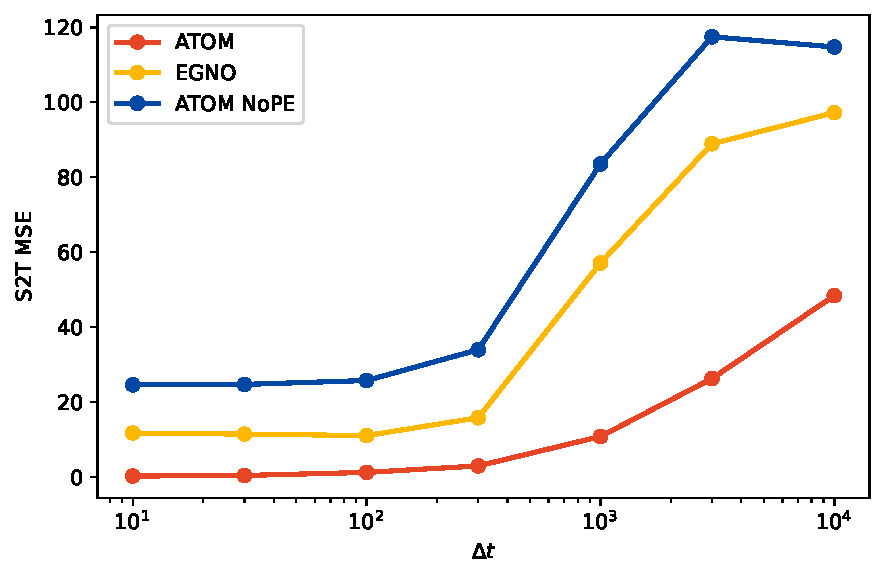
\includegraphics[width=\linewidth]{Figures/invariances/t_invariance_multi.pdf}
    \caption{Pretrained ({\(\Delta T = 3000\)}, ID) multitask S2T \gls{mse} across varying \(\Delta T\) values.}
    \label{fig:delta_t_invariance}
\end{minipage}
\hfill
\begin{minipage}[t]{0.45\linewidth}
    \centering
    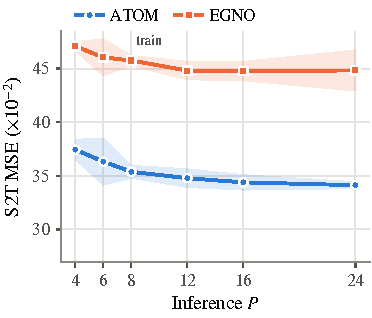
\includegraphics[width=\linewidth]{Figures/invariances/p_invariance_multi.pdf}
    \caption{{Pretrained (\(P=8\))} \gls{atoms} and \gls{egno} are discretization invariant, showing stable S2T \gls{mse}.}
    \label{fig:p_invariance}
\end{minipage}
\hfill
\label{fig:invariances}
\end{figure}

\subsection{Ablation studies}
\label{sec:ablations}

We perform extensive ablations to assess each design choice in \gls{atoms}. For single-task performance (Fig.~\ref{fig:MD17_ablation}) and multitask performance (Fig.~\ref{fig:TG80_ablation}), we independently toggle components and measure their contributions. Our analysis focuses on equivariant lifting, T-RoPE, input-noise augmentation, heterogeneous attention, and random-walk positional encoding (under multitask pretraining).
% . Single-task and multi-task results are shown in \Cref{fig:MD17_ablation}, and multi-task results can be found in \Cref{fig:TG80_ablation}.




\FPeval{\NoEquivariantLiftingvsDefault}{round(5.92 - 5.27, 2)}
\FPeval{\FullyEquivariantvsDefault}{round(7.18 - 5.27, 2)}
\FPeval{\AtomRotationPenalty}{round(73.04 / 6.76, 2)}
\FPeval{\NoLiftRotationPenalty}{round(660.97 / 33.44, 2)}

\begin{wrapfigure}{r}{0.48\textwidth}
    \centering
    \setlength{\extrarowheight}{1pt}   % try 0.5–2pt
    \vspace{-10pt}
    \captionof{table}{S2T MSE (\(\times 10^{-2}\)) of a fixed input frame rotated and unrotated by an \(\mathrm{SO}(3)\) matrix.}
    \resizebox{\linewidth}{!}{%
    \begin{tabular}{l cc}
        \toprule
        & ATOM & No equivariant Lift \\
        \midrule
        Unrotated & \(6.76{\scriptstyle \pm0.69}\) & \(33.44{\scriptstyle \pm23.42}\) \\
        Rotated & \(73.04{\scriptstyle \pm27.01}\) & \(660.97{\scriptstyle \pm945.86}\) \\
        \midrule
        Increase & \(66.28{\scriptstyle \pm26.32}\) & \(627.53{\scriptstyle \pm926.53}\) \\
        \rowcolor{gray!20} Rotation penalty (\(\times\)) & \(\AtomRotationPenalty\) & \(\NoLiftRotationPenalty\) \\
        \bottomrule
    \end{tabular}
    }
    \label{tab:equivariance_error}
\end{wrapfigure}

\textbf{Equivariant lifting.} We assess the quasi-equivariant design against a non-equivariant ATOM. As shown in \Cref{fig:MD17_ablation}, replacing the equivariant lifting introduced in \Cref{sec:equivariant_lifting} with standard linear layers (no equivariant lifting) degrades the performance of \gls{atoms}, increasing S2T \gls{mse} by \NoEquivariantLiftingvsDefault{}. \Cref{tab:equivariance_error} further quantifies sensitivity to \(\mathrm{SO}(3)\) rotations: ATOM's S2T \gls{mse} increases by \(\AtomRotationPenalty\times\) under rotation, compared to \(\NoLiftRotationPenalty\times\) without equivariant lifting. Notably, the fully-equivariant variant of \gls{atoms}, described in appendix \Cref{sec:fully_equivariant}, also underperforms \gls{atoms} in single-task learning (\Cref{fig:MD17_ablation}), increasing S2T \gls{mse} by \FullyEquivariantvsDefault{}; we report its multitask performance in appendix \Cref{sec:fully_equivariant}. This aligns with recent findings on relaxed equivariance, suggesting that strict equivariance can limit model capacity and complicate the optimization process \cite{elhag_relaxed_2025}. We present estimates of the quasi-equivariance \(\varepsilon\) in \Cref{app:quasi_equivariance_mc}.

\FPeval{\CrossAttvsStdAtt}{round(5.99 - 5.27, 2)}
\textbf{Heterogeneous attention.} We find that substituting heterogeneous temporal attention with standard self-attention on the phase space features increases S2T MSE by \CrossAttvsStdAtt{}, suggesting that cross-attention enables access to non-trivial feature interactions.

% To verify the importance of our heterogeneous temporal attention, we train \gls{atoms} with standard self-attention on the phase space features and find it degrades performance, by \CrossAttvsStdAtt{} in S2S \gls{mse}. 
% We find \gls{gnot} \cite{hao_gnot_2023} linear attention performs similarly to our method.

% No-TROPE - Default
\FPeval{\NoPEvsDefault}{round(46.05 - 35.47, 2)}
\FPeval{\NoPEvsDefaultST}{round(6.35 - 5.27, 2)}
\textbf{\gls{trope}.} 
In the single-task regime with fixed $\Delta T$ (\Cref{fig:MD17_ablation}), disabling \gls{trope} (NoPE) increases S2T \gls{mse} by \NoPEvsDefaultST{}. With stochastic $\Delta T$, disabling \gls{trope} (NoPE) increases \gls{mse} by \NoPEvsDefault{}, consistent with \gls{atoms} leveraging the \(\tau\) parameter to encode  variable time gaps (\Cref{fig:TG80_ablation}).  An \gls{egno}-style sinusoidal positional encoding produces a similar performance degradation.


% As expected, \gls{trope} has a negligible effect in the single-task setting with fixed \(\Delta T\) as it reduces to a fixed rotational shift. 
% Under stochastic \(\Delta T\), however, disabling \gls{trope} (NoPE) increases \gls{mse} by \NoPEvsDefault{},  An \gls{egno}-style sinusoidal positional encoding produces a similar performance degradation.

\textbf{Input-noise augmentation.}
\FPeval{\NoNoisevsDefault}{round(6.53 - 5.27, 2)}
We also test the utility of input-noise augmentation as in \Cref{sec:label_noise}. From \Cref{fig:MD17_ablation}, we observe that removing augmented noise from the position and velocity features increased S2T \gls{mse} by \NoNoisevsDefault{}. For the multitask ablation on TG80, we disable input-noise augmentation, as the dataset is designed to be numerically stable with small noise.

\textbf{RWPE.} We assess random-walk positional encoding (RWPE) in the multitask pretraining. Figure~\ref{fig:TG80_ablation} indicates that RWPE facilitates molecule identification, yielding improved multitask performance.

% \textbf{Further architectural elements.}
% We found that the delta update, as described in \Cref{sec:delta_prediction}, provided no improvement compared to our MD17 baseline and that learnable value residuals (\Cref{sec:value_residuals}) \cite{zhou_value_2024} have a minor positive effect on \gls{mse}.

\begin{figure}[t]
\centering
\begin{minipage}[t]{0.46\linewidth}
    \centering
    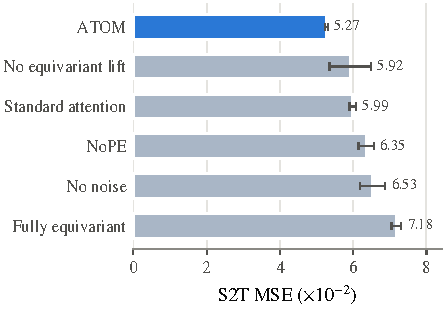
\includegraphics[width=\linewidth]{Figures/ablation_MD17_ST_reduced.pdf}
    \caption{\gls{atoms} ablation on MD17 Aspirin.}
    \label{fig:MD17_ablation}
\end{minipage}
\hfill
\begin{minipage}[t]{0.46\linewidth}
    \centering
    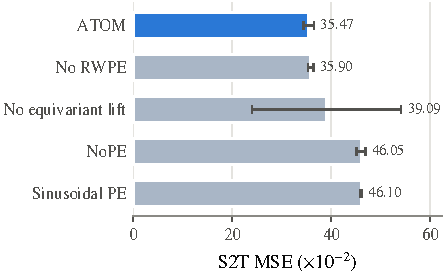
\includegraphics[width=\linewidth]{Figures/ablation_TG80_MT.pdf}
    \caption{\gls{atoms} ablation on TG80 Cluster 1.}
    \label{fig:TG80_ablation}
\end{minipage}
\label{fig:ablations}
\end{figure}

\section{Conclusions}

In this work, we demonstrate that carefully designed transformer neural operators enable zero-shot generalization to unseen chemical dynamics. Our experiments on MD17 demonstrate continued good single-task performance, and we present the first molecular neural operator that can successfully learn large molecule dynamics using MD22. Our multitask experiments show that our method learns transferable dynamics knowledge, even without explicit graph representations. In combination with our TG80 dataset, we provide a large-scale open-source benchmark and baselines to evaluate future models and spur further operator research with concrete scientific applicability.


\paragraph{Limitations} We remark that TG80 does not contain trajectories for large molecules with more than 15 heavy atoms, despite their obvious chemical and pharmacological relevance. In follow-up work, we intend to enrich TG80 with such molecules, calculated with a higher-resolution DFT basis set, \(\omega\)B97X-3c \cite{muller_omegab97x-3c_2023}. Regarding \gls{atoms}, it lacks an explicit energy-based inductive bias, which may permit long-horizon drift. A natural extension is therefore a framewise energy head \(E_\theta(\mathbf{x}_{t_p})\) with force supervision \(\mathbf{F}_{t_p}=-\nabla_{\mathbf{x}_{t_p}}E_\theta(\mathbf{x}_{t_p})\). {This energy term also defines the drift in the Langevin dynamics, where an additional stochastic term accounts for thermal perturbations of atomic positions. Incorporating such physics-informed stochastic dynamics into our operator learning framework is a natural next step, and we view this as a promising direction for future \gls{md} research.}
% unlike some neural force field and Hamiltonian approaches. 


% \section{Reproducibility Statement}
% We provide full code, including ATOM, EGNO and EGNN baseline models along with their checkpoints and original results files.

% \newpage

% \printbibliography


\section*{Reproducibility Statement}
We provide experiment details, such as choice of hyperparameters and other training configurations in Appendix \ref{sect:details}. In addition, we will release the TG80 dataset upon acceptance under MIT license for reproducibility.
\newpage

\bibliographystyle{ICLR2026/iclr2026_conference}
\bibliography{library}

\appendix
\clearpage
% \EScomment{


\renewcommand{\contentsname}{\textsc{Appendices}}
% \renewcommand{\cfttoctitlefont}{\normalfont\large}
% \renewcommand{\cftsecfont}{\normalfont} 
% \renewcommand{\cftsecpagefont}{\normalfont}
\addcontentsline{toc}{section}{Appendices}  
\addtocontents{toc}{\protect\setcounter{tocdepth}{4}} 
\tableofcontents 


\clearpage
\section{LLM Acknowledgment}

The authors acknowledge the use of LLM for grammar corrections and for improving the clarity of the manuscript. The LLM was not used for generating original ideas, content, or experimental results. All conceptual contributions, analyses, and conclusions presented in this work are entirely from the authors.

\section{Background}

This section provides an introduction to the preliminaries of group theory. 

\subsection{Groups}
\label{sec:groups}
A group \( (G, \circ) \) consists of a non-empty set \( G \) and a binary operation \(\circ: G \times G \to G\) satisfying the following axioms:
\begin{enumerate}
    \item \textbf{Closure:} For all \( a, b \in G \), the result of the operation \( a \circ b \) is also in \( G \): \( a \circ b \in G \).
    \item \textbf{Identity Element:} There exists an element \( e \in G \) such that, for all \( a \in G \), \( a \circ e = e \circ a = a \).
    \item \textbf{Associativity:} For all \( a, b, c \in G \), \( (a \circ b) \circ c = a \circ (b \circ c) \).
    \item \textbf{Inverses:} For each \( a \in G \), there exists an element \( a^{-1} \in G \) such that \( a \circ a^{-1} = a^{-1} \circ a = e \).
\end{enumerate}

In general, not all groups are abelian. That is, the binary operation \(\circ\) does not necessarily commute:  
$
g \circ h = h \circ g,  \forall g,h \in G.
$

\subsection{Group Representations}
\label{sec:group_representations}
A group representation is a homomorphism  \(\rho: G \to GL(V)\) that assigns an \(n \times n\) matrix to each group element \(g \in G\), realizing it as a linear transformation. Representations must preserve the binary operation for all members of the group \(G\) such that:
\[
\rho(g \circ h) = \rho(g) \rho (h), \quad \forall g,h \in G.
\]

A representation \(\rho(g)\) is reducible if it can be represented as the direct sum of other representations:
\[
\rho(g) = \rho_1(g) \oplus \rho_2(g), \quad \forall g \in G.
\]

For example, a reducible \(4 \times 4\) representation of \(SU(2)\) can be decomposed into two \(2 \times 2\) sub-representations:
\[
\rho(g) =
\begin{bmatrix}
\rho_1(g) & 0 \\
0 & \rho_2(g)
\end{bmatrix}, \quad \forall g \in SU(2),
\]

where \(\rho_1(g)\) and \(\rho_2(g)\) are the following irreducible representations of \(SU(2)\):

\[
\rho_1(g) =
\begin{bmatrix}
e^{i\theta} & 0 \\
0 & e^{-i\theta}
\end{bmatrix}, \quad
\rho_2(g) =
\begin{bmatrix}
e^{i\phi} & 0 \\
0 & e^{-i\phi}
\end{bmatrix}.
\]
By contrast, irreducible representations or \textit{irreps} cannot be represented as such a direct sum. Formally, they have no non-trivial invariant subspaces \(W \subset V\) such that \(\rho(g)W \subset W, \forall g \in G\).

Representing inputs as irreps ensures equivariance by constraining each feature to transform predictably under group actions. Given \( V = \bigoplus_{i} V_i \) with irreps \( V_i \), the transformation of an input \( x \in V \) under \( g \in G \) is:  
\[
\rho(g)x = \bigoplus_{i} \rho_i(g)x_i.
\]  
Each component \( x_i \) transforms independently according to \(\rho_i\), preserving symmetry. Scalars remain invariant, while vectors rotate according to standard representations. This decomposition prevents the mixing of differently transforming features, ensuring that all subsequent operations, linear or non-linear, respect the group’s symmetry, thereby maintaining equivariance throughout the network.

% \subsection{Tensor Products}
% \label{sec:tensor_products}
% Equivariance imposes strict constraints on how neural network operations can transform input features. By Schur's lemma, given irreps \(\rho_i\) and \(\rho_j\), a linear map (e.g., weights) \(T \colon V_i \to V_j\) satisfying equivariance
% \[
% T\rho_i(g) = \rho_j(g)T, \quad \forall g \in G
% \]
% must either be the zero map or an isomorphism \(\rho_i \cong \rho_j\). This initially presents a problem for our architecture, as we are prevented from mixing features between our positions and velocities -- precisely the goal of our phase space construction.

% To circumvent this and achieve meaningful equivariance-preserving feature mixing, we employ tensor products. 
% Given two lifted embeddings \(\tilde{\mathbf{x}}, \tilde{\mathbf{v}} \in V\), each transforming according to their irreps, their tensor product is defined as
% \[
% g \cdot (\tilde{\mathbf{x}} \otimes \tilde{\mathbf{v}})
% =
% (\rho_V (g) \tilde{\mathbf{x}}) \otimes (\rho_V (g) \tilde{\mathbf{v}}).
% \]

% \[
% \tilde{\mathbf{x}} \otimes \tilde{\mathbf{v}}
% \mapsto
% (\rho_{\tilde{\mathbf{x}}} \otimes \rho_{\tilde{\mathbf{v}}})(g)(\tilde{\mathbf{x}} \otimes \tilde{\mathbf{v}})
% =
% (\rho_{\tilde{\mathbf{x}}}(g)\tilde{\mathbf{x}}) \otimes (\rho_{\tilde{\mathbf{v}}}(g) \tilde{\mathbf{v}}).
% \]
Intuitively, the tensor products capture interactions between features in a manner akin to multiplication, producing a higher-dimensional representation.
Crucially, this new representation is reducible, so we may decompose it into irreps:
\[
V \otimes V \cong \bigoplus_k V_k.
\]
It is this decomposition that allows the network to project onto individual irreps, achieving non-trivial feature mixing whilst preserving symmetry constraints.
% }

\section{Datasets}
\label{sec:dataset_construction}

We present a visualization of a sample trajectory of uracil from three datasets in Figure \ref{fig:uracil_trajectory}.

% \begin{wrapfigure}{r}{0.6\textwidth}
%     \vspace{-1em}
%     \centering
%     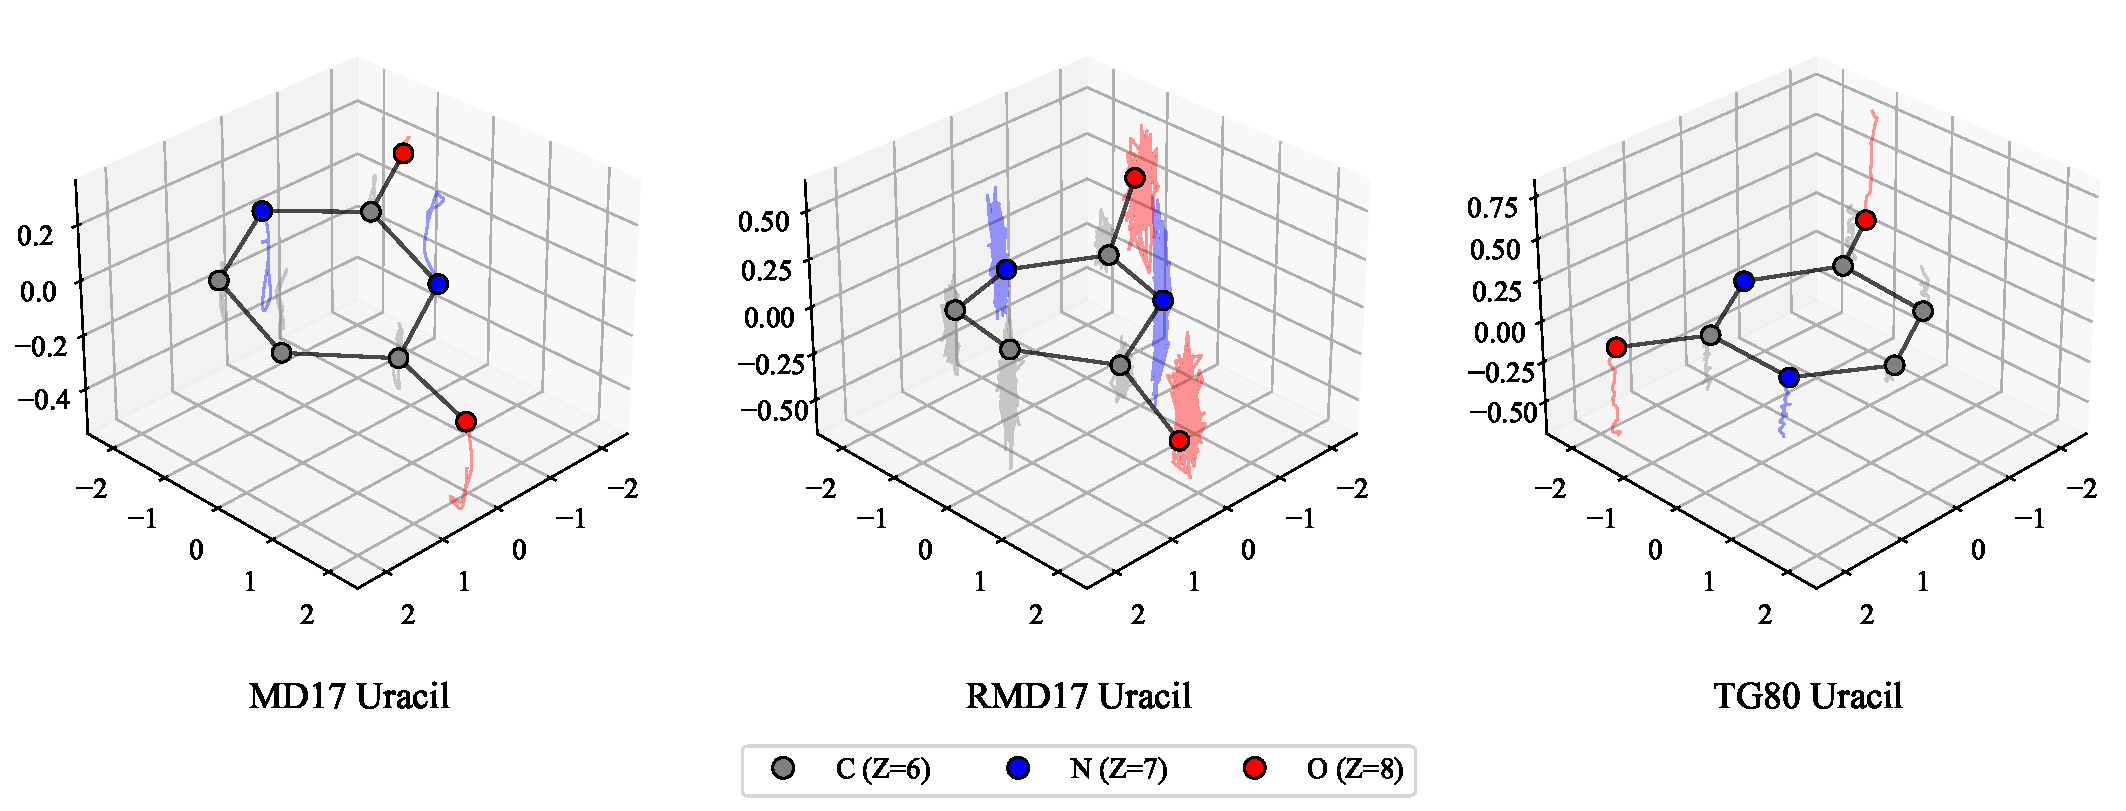
\includegraphics[width=\linewidth]{Figures/dataset/uracil_comparison.pdf}
%     \caption{3000 timesteps of uracil trajectory from MD17, RMD17, and TG80.}
%     \label{fig:uracil_trajectory}
% \end{wrapfigure}

\begin{figure}[h]
    \centering
    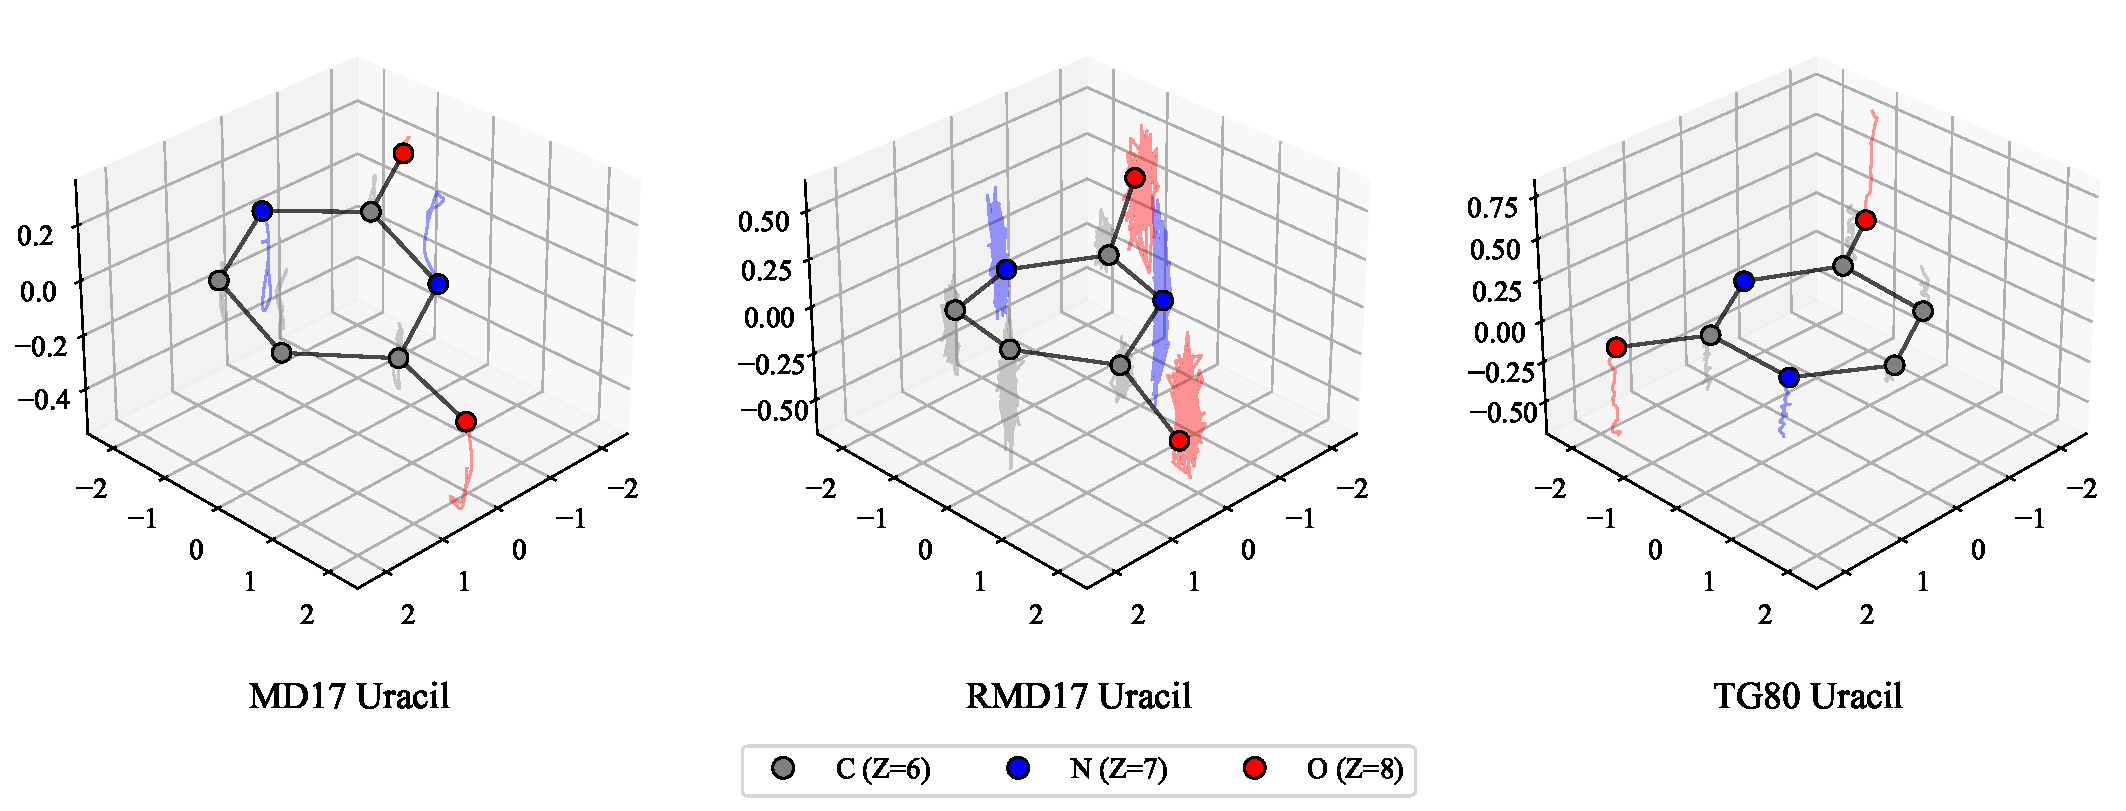
\includegraphics[width=0.8\linewidth]{Figures/dataset/uracil_comparison.pdf}
    \caption{3000 timesteps of uracil trajectory from MD17, RMD17, and TG80.}
    \label{fig:uracil_trajectory}
\end{figure}


\subsection{Licences}
\begin{table}[ht]
\centering
\caption{Dataset sources and licenses. We release TG80 under the MIT license.}
\label{tab:dataset_sources}
\rowcolors{2}{gray!10}{white}
\resizebox{\linewidth}{!}{
    \begin{tabular}{lll}
    \toprule
    \textbf{Dataset} & \textbf{Source} & \textbf{License} \\
    \midrule
    MD17            & \url{https://www.sgdml.org/} & \texttt{CC BY 4.0}\\
    RMD17           & \url{https://archive.materialscloud.org/record/2020.82} & \texttt{CC Zero V1.0 Universal} \\
    MD22           & \url{https://www.sgdml.org/} & \texttt{CC BY 4.0} \\
    TG80            & \url{https://ses.library.usyd.edu.au/handle/2123/35120} & \texttt{MIT}\\
    \bottomrule
    \end{tabular}}
\end{table}

\subsection{Model Inputs and the Dataloader}
\label{sec:dataloader}
Our compound representations follow \cite{shi_learning_2021, xu_equivariant_2024}. We model hydrogen atoms implicitly and concatenate the position and velocity norms for each node \(i\) with their respective vectors. Unlike their implementations, we avoid explicit graph construction and do not include edge labels describing atomic bond geometries.

We duplicate all frames \(\mathcal{G}^{(t)} \to \{\mathcal{G}^{(t)}\}^{P}\) during dataset initialization, producing a five-fold improvement in throughput compared to previous dataloaders in \Cref{tab:dataloader_perf}. 

\begin{table}[ht]
    \centering
    \caption{Mean time (seconds) to produce 10\,000 batches over 100 benchmark runs. Batch size = 100, 500 samples, \(\Delta t = 3000\), 500 warmup batches.}
    \label{tab:dataloader_perf}
    \begin{tabular}{lcccc}
        \toprule
         & Aspirin & Ethanol & Naphthalene & Toluene \\
         \midrule
         \gls{egno} & \(0.060{\scriptstyle \pm0.024}\) & \(0.024{\scriptstyle \pm0.016}\) & \(0.056{\scriptstyle \pm0.024}\) & \(0.039{\scriptstyle \pm0.024}\) \\
         \gls{atoms} & \(\textbf{0.005}{\scriptstyle \pm0.002}\) & \(\textbf{0.007}{\scriptstyle \pm0.002}\) & \(\textbf{0.008}{\scriptstyle \pm0.004}\) & \(\textbf{0.006}{\scriptstyle \pm0.002}\) \\
         \bottomrule
    \end{tabular}
\end{table}

\newpage
\subsection{Numerical Stability}
We evaluate the numerical stability of MD17, RMD17, and TG80. MD17 benzene exhibits substantially higher position variance in \Cref{fig:MD17_numerical_quality}, which is also partially visible in the consistent motion trails shown in \Cref{fig:MD17_trajectories}. RMD17 exhibits improved stability, with no position variance exceeding \(10\)~\AA{}\(^2\). TG80 shows the lowest median position variance of all datasets, and expectedly includes more molecules with high per-step displacement variance (due to more complex sterically hindered geometries).
\begin{figure}[H]
    \begin{subfigure}{0.49\textwidth}
        \centering
        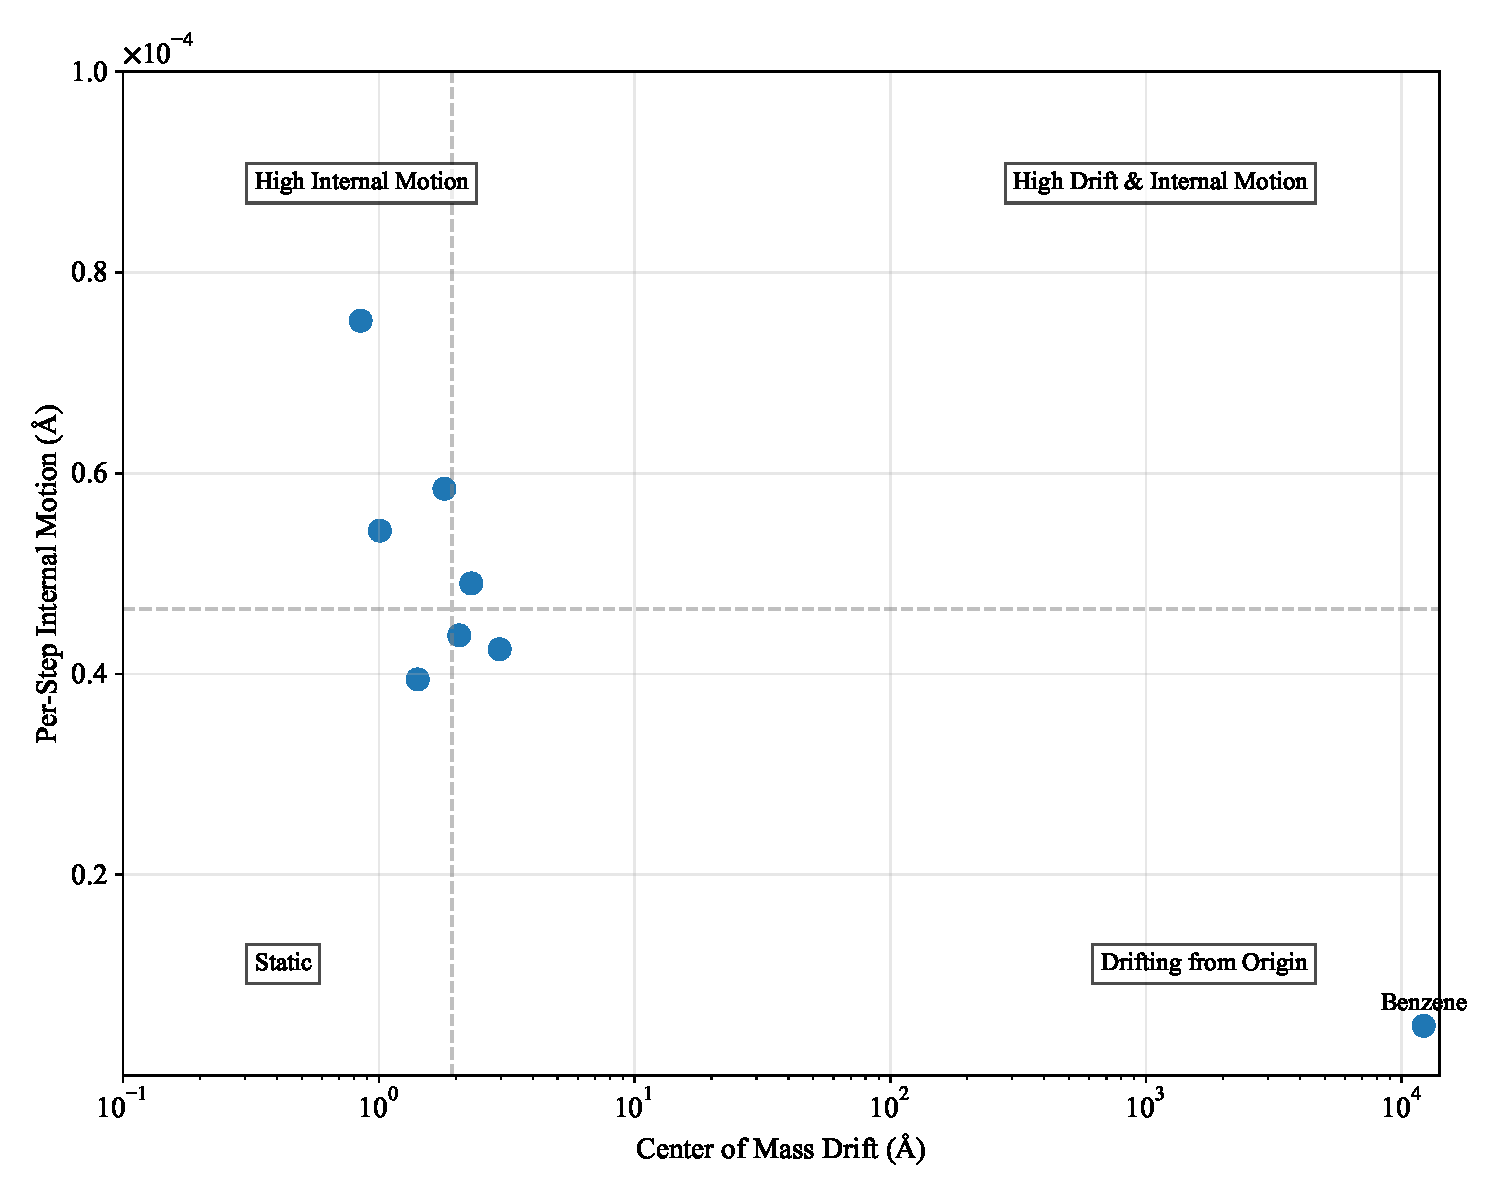
\includegraphics[width=\linewidth]{Figures/dataset/md17_molecule_behavior_comparison.pdf}
        \caption{MD17 molecules are largely consistent, except for benzene, which exhibits substantially higher position variance.}
        \label{fig:MD17_numerical_quality}
    \end{subfigure}
    \hspace{0.02\textwidth}
    \begin{subfigure}{0.49\textwidth}
        \centering
        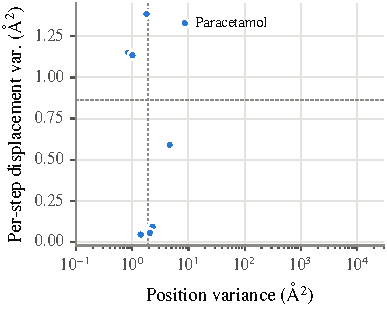
\includegraphics[width=\linewidth]{Figures/dataset/rmd17_molecule_behavior_comparison.pdf}
        \caption{RMD17 molecules are more numerically stable, supporting their use in future benchmarks.}
        \label{fig:RMD17_numerical_quality}
    \end{subfigure}
    \begin{subfigure}{\textwidth}
        \centering
        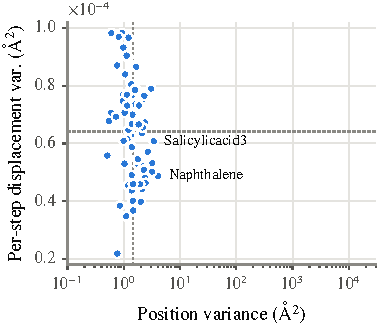
\includegraphics[width=\linewidth]{Figures/dataset/tg80_molecule_behavior_comparison.pdf}
        \caption{TG80 molecules exhibit the lowest position variance among the evaluated MD datasets.}
        \label{fig:TG80_numerical_quality}
    \end{subfigure}
    \caption{Comparison of numerical stability across MD17, RMD17, and TG80 datasets. Each point is one molecule: the x-axis is the variance of all Cartesian coordinates over the trajectory and the y-axis is the mean per-atom variance of the per-step displacement magnitude. Dashed lines denote the medians; datapoints more than two standard deviations from the median are annotated.}
    \label{fig:numerical_stability}
\end{figure}

\subsection{TG80 Generation Algorithm}
\label{sec:tg80_algorithm}
{We first recall the definition of Tanimoto \(\operatorname{T}\) similarity between two bit vectors \(X,Y\) as
\[
\operatorname{T}(X,Y) = \frac{|X \cap Y|}{|X \cup Y|},
\]
which is identical to the definition of the Jaccard similarity in this case \cite{rogers_computer_1960}.}

To generate TG80, we randomly shuffled the PubChem dataset, then iterated through all compounds until 40 were found that matched the following criteria:
\begin{wrapfigure}{r}{0.4\linewidth}
  \vspace{1em}
  \centering
  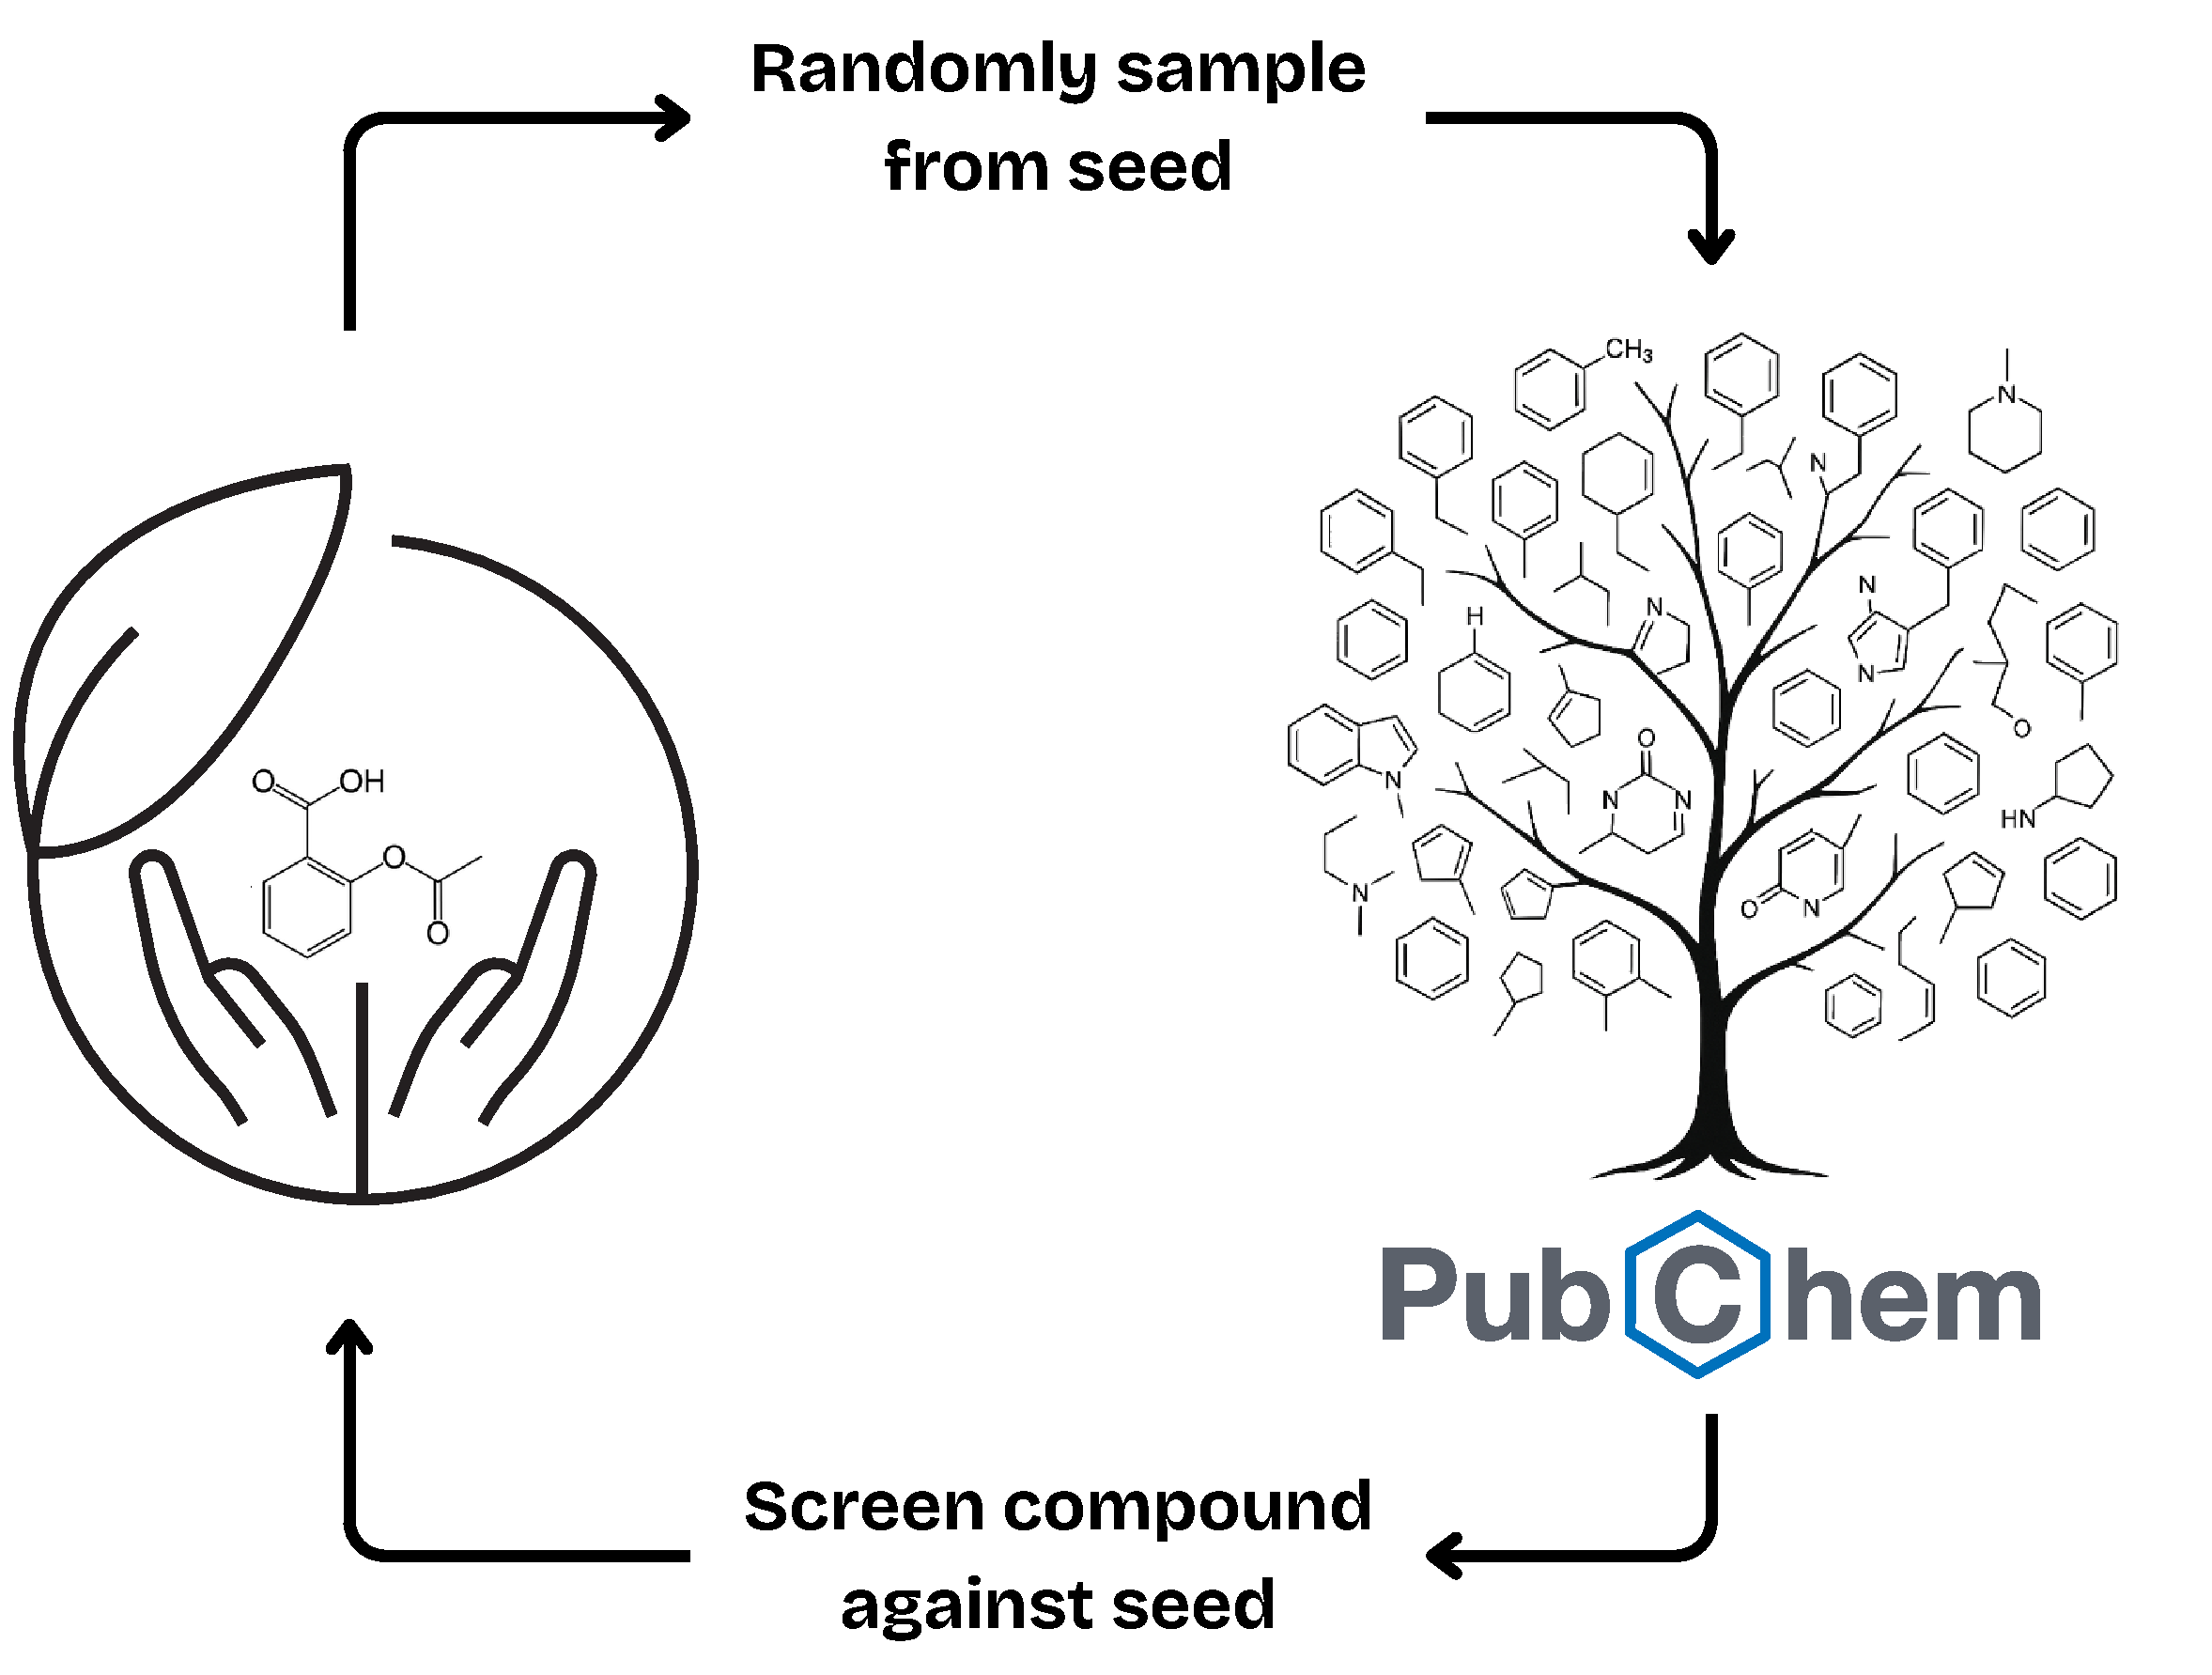
\includegraphics[width=\linewidth]{Figures/TG80.pdf}
  \caption{{Construction of TG80 from an initial seed using the PubChem database.}}
  \label{fig:dataset_construction}
  \vspace{-5em}
\end{wrapfigure}
{\begin{enumerate}
    \item \gls{smiles} encode a valid molecular structure
    \item No more heavy atoms than the corresponding seed molecule
    \item Only contain \(\{\text{C, H, O, N}\}\) atoms
    \item No more than five oxygen atoms
    \item No more than three nitrogen atoms
    \item No disconnected molecular fragments (e.g., salts)
    \item Tanimoto distance \(1-\operatorname{T}\) to at least one seed molecule between 0.875 and 0.925 (similarity between 0.075 and 0.125)
    \item Tanimoto similarity to any previously selected molecule is no more than 0.2
\end{enumerate}}
This selection procedure adds molecules that are only weakly similar to the seed set, and prevents convergence to highly similar molecules across selections. The criteria apply to the 40 selected molecules only; the 40 seed molecules include five compounds containing Cl or S (chloroform, 1,2-dichloroethane, chlorobenzene, ethanethiol and benzothiophene).

{Only 2,488 of the 173 million in the PubChem library satisfied the filtration criteria above. This low yield largely reflects the cumulative effect of criterion 8: as more molecules are added, it becomes harder to find candidates sufficiently dissimilar to all prior selections. Dataset generation code is available at \url{https://github.com/luke-a-thompson/ATOM/blob/main/data/chemical_sieve.py}.}
% \url{https://github.com/luke-a-thompson/ATOM/blob/main/data/chemical_sieve.py}

\subsection{Molecular Dynamics Simulations}
We present a complete overview of the \gls{dft} parameters used to generate MD17 \cite{chmiela_machine_2017}, RMD17 \cite{christensen_role_2020}, MD22 \cite{chmiela_accurate_2023}, and TG80.
\begin{table}[H]
    \centering
    \caption{An overview of the methodologies used to generate the \gls{md} datasets featured.}
    \label{tab:dft_techniques}
    \begin{tabular}{lccccc}
        \toprule
        & \gls{dft} Functional & Dispersion Corrections & Basis set & Timestep & Temperature \\
        \midrule
        MD17 & PBE & TS & NAO & 0.5 fs & 500K  \\
        RMD17 & PBE & None & def2-SVP & 0.5 fs & 500K  \\
        MD22 & PBE & MBD & NAO & 1.0 fs & 500K \\
        TG80 & PBE & \(\Delta 4\) & def2-SVP & 1.0 fs & 300K \\
        \bottomrule
    \end{tabular}
\end{table}

\newpage
\section{Architectural Details}
In this section, we discuss the finer architectural details of \gls{atoms} and the architectural adjustments made for our ablations.
\subsection{Fully Equivariant ATOM}
\label{sec:fully_equivariant}
To achieve the full equivariance discussed in \Cref{fig:MD17_ablation}, we employ a canonicalization network approach, which removes Euclidean gauge before learning and then reinstates it afterwards \cite{kaba_equivariance_2023}. This preserves equivariance of the whole network, even with the use of non-equivariant architectures in the trunk. This provides a controlled comparison between equivariant and non-equivariant \gls{atoms}: it enforces equivariance by construction while otherwise keeping the core architecture unchanged.

We first make data translation equivalent by centering
\begin{equation}
    \mu = \frac{1}{N}\sum_{i=1}^N x_i,
    \qquad
    \bar x_i = x_i - \mu.
\end{equation}
We then remove rotations by aligning to the second moment
\begin{equation}
    S = \tfrac{1}{N}\sum_{i=1}^N \bar x_i \bar x_i^\top
    = \sum_{k=1}^3 \lambda_k e_k e_k^\top
    \quad (\lambda_1 \ge \lambda_2 \ge \lambda_3),
\end{equation}
and choose \(e_1\) as the principal axis and orthonormalise
\begin{equation}
e_2 \leftarrow \frac{e_2 - (e_2^\top e_1)e_1}{\|e_2 - (e_2^\top e_1)e_1\|}, \qquad e_3  = e_1 \times e_2.
\end{equation}
We can then form \(Q = [e_1, e_2, e_3] \in \mathrm{SO}(3)\) and canonicalise
\begin{equation}
    \tilde x_i = (x_i-\mu)\,Q,\qquad \tilde v_i = v_i\,Q.
\end{equation}
We fix the eigenvector sign ambiguity using the chirality pseudoscalar \(c_0=\sum_{i=1}^N x_i\times v_i\) at the reference time (flip \(e_1\) to satisfy \(e_1^\top c_0\ge 0\), then adjust \(e_2,e_3\) jointly to keep right-handedness).
Let \(F\) be an arbitrary trunk acting in the canonical frame; with per-atom canonical outputs \(\hat y_i=F(\{\tilde x_j,\tilde v_j\}_{j=1}^N)_i\), we decanonicalise by
\begin{equation}
    y_i=\hat y_i\,Q^\top+\mu.
\end{equation}

This results in exact \(\mathrm{SE}(3)\)-equivariance \citep{kaba_equivariance_2023} and permits non-equivariant trunks.

On TG80 multitask learning (Cluster 1, OOD), the fully-equivariant variant reaches an S2T \gls{mse} of \(32.08{\scriptstyle \pm1.18}\times10^{-2}\), compared to \(35.47{\scriptstyle \pm0.53}\times10^{-2}\) for \gls{atoms}.

\subsection{Random-Walk Positional Encodings}
\label{sec:positional_encoding}
In the multitask case, we add row-normalized \gls{rwpe} to equip \gls{atoms} and \gls{egno} with multiscale connectivity features, enhancing their ability to distinguish non-isomorphic graphs \cite{dwivedi_graph_2022, ma_graph_2023}. We first form a \(\varepsilon\)-neighborhood graph from our pointclouds as:
\begin{equation}
    G = (V,E), \quad V = \{i\}, \quad E = \{(i,j): \|(x,y,z)_i-(x,y,z)_j\|_2 < \varepsilon\}.
\end{equation}
We set \(\varepsilon = 1.6\), as covalent bonds typically range from 1.14 \AA{} to 2.0 \AA{} in length \cite{lobato_highs_2021} and highlight that this construction does not necessitate prior knowledge of the graph structure.

Let $\mathbf{A} \in \mathbb{R}^{n \times n}$ denote the adjacency matrix of this graph, and let $\mathbf{D} = \text{diag}(\mathbf{A}\mathbf{1})$ represent its degree matrix. We construct the random walk transition matrix as \(\mathbf{M} = \mathbf{D}^{-1} \mathbf{A}\) then compute matrix powers of $\mathbf{M}$ up to a maximum walk-length $K$, defining the self-return probabilities for each node as
\begin{equation}
    p_i^{(k)} = \left(\mathbf{M}^k\right)_{ii}, \quad k = 1, \dots, K.
\end{equation}

These probabilities are collected into vectors $\mathbf{p}_i \in \mathbb{R}^{K}$ and concatenated with the phase space to form \(\hat{\mathbf{z}} = \left(\mathbf{v} \parallel \mathcal{Z} \parallel \mathbf{p}\right) \in W_\text{in}\). Here, the input feature space is redefined as \(W_\text{in} = V_\text{in} \oplus \rho_0^\text{even} \oplus \left(\rho_0^\text{even} \otimes \mathbb{R}^{K}\right)\), and the subsequent equivariant maps are modified in kind.

\subsection{Value-residual Learning}
\label{sec:value_residuals}
We employ value-residual learning wherein each transformer block receives the output of the first block via a residual connection to stabilize training and information flow through the network \cite{zhou_value_2024}. Inspired by \cite{jordan_nanogpt_2024}, we add a learned coefficient to weight this residual. Here, \(v\) denotes the current block's value output, and \(v_1\) represents the initial block's value. A learnable parameter \(\alpha\) is passed through a sigmoid to obtain the weighting coefficient:
\begin{equation}
    \lambda = \sigma(\alpha).
\end{equation}
The combined output is then given by:
\begin{equation}
    v = \lambda\,v + (1 - \lambda)\,v_1.
\end{equation}
In practice, we lock the first block's \(\lambda\) value to \(0.5\). 

% We report the learned \(\lambda\) values in \Cref{fig:lambda_values}.

% \begin{figure}[H]
%     \begin{subfigure}{0.48\textwidth}
%         \centering
%         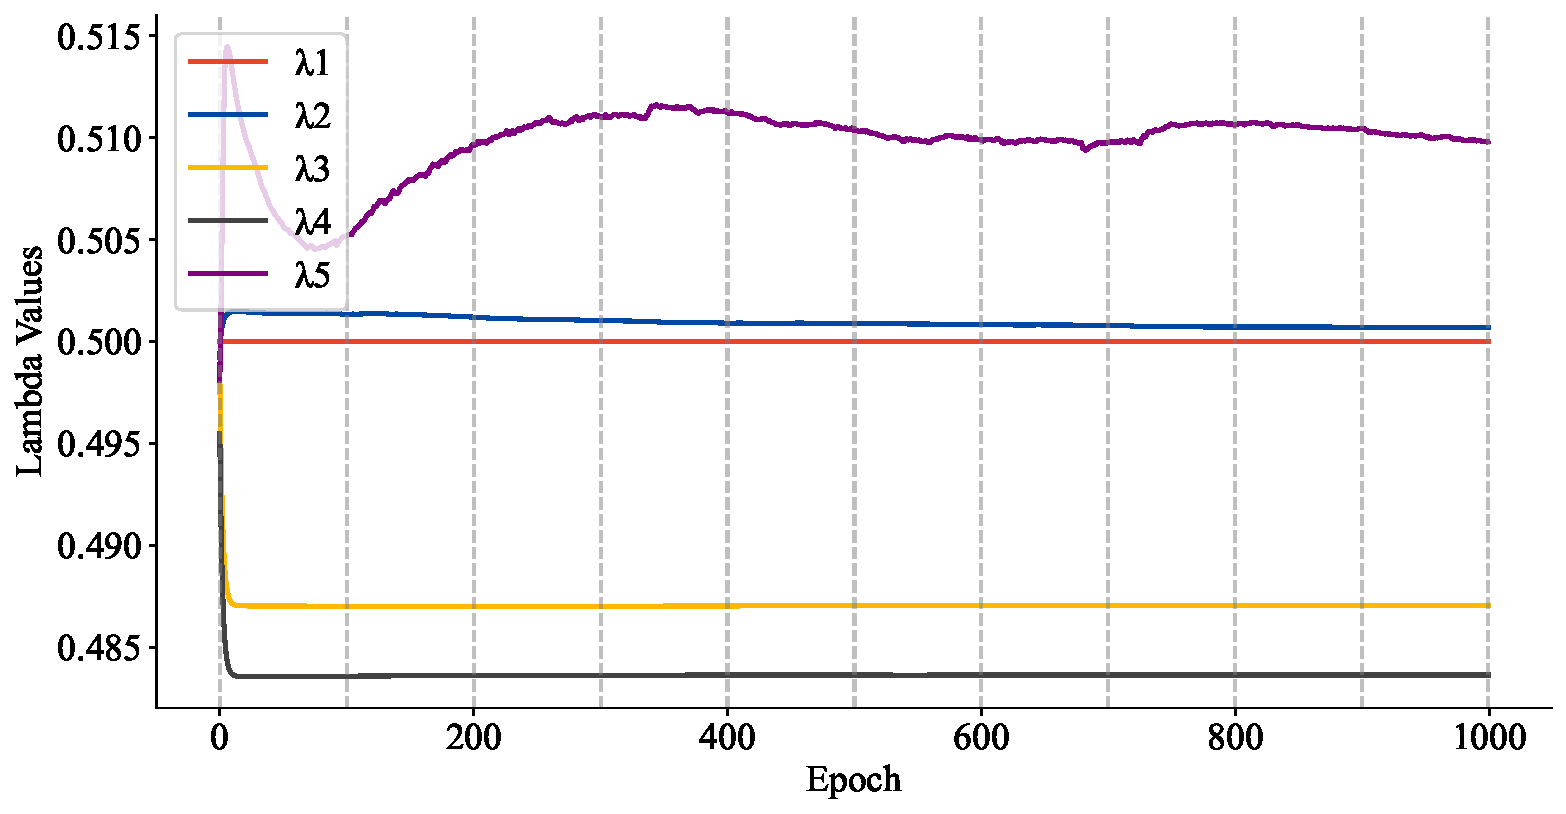
\includegraphics[width=\textwidth]{Figures/lambda_residuals/lambda_values_aspirin.pdf}
%         \caption{Aspirin}
%     \end{subfigure}
%     \hfill
%     \begin{subfigure}{0.48\textwidth}
%         \centering
%         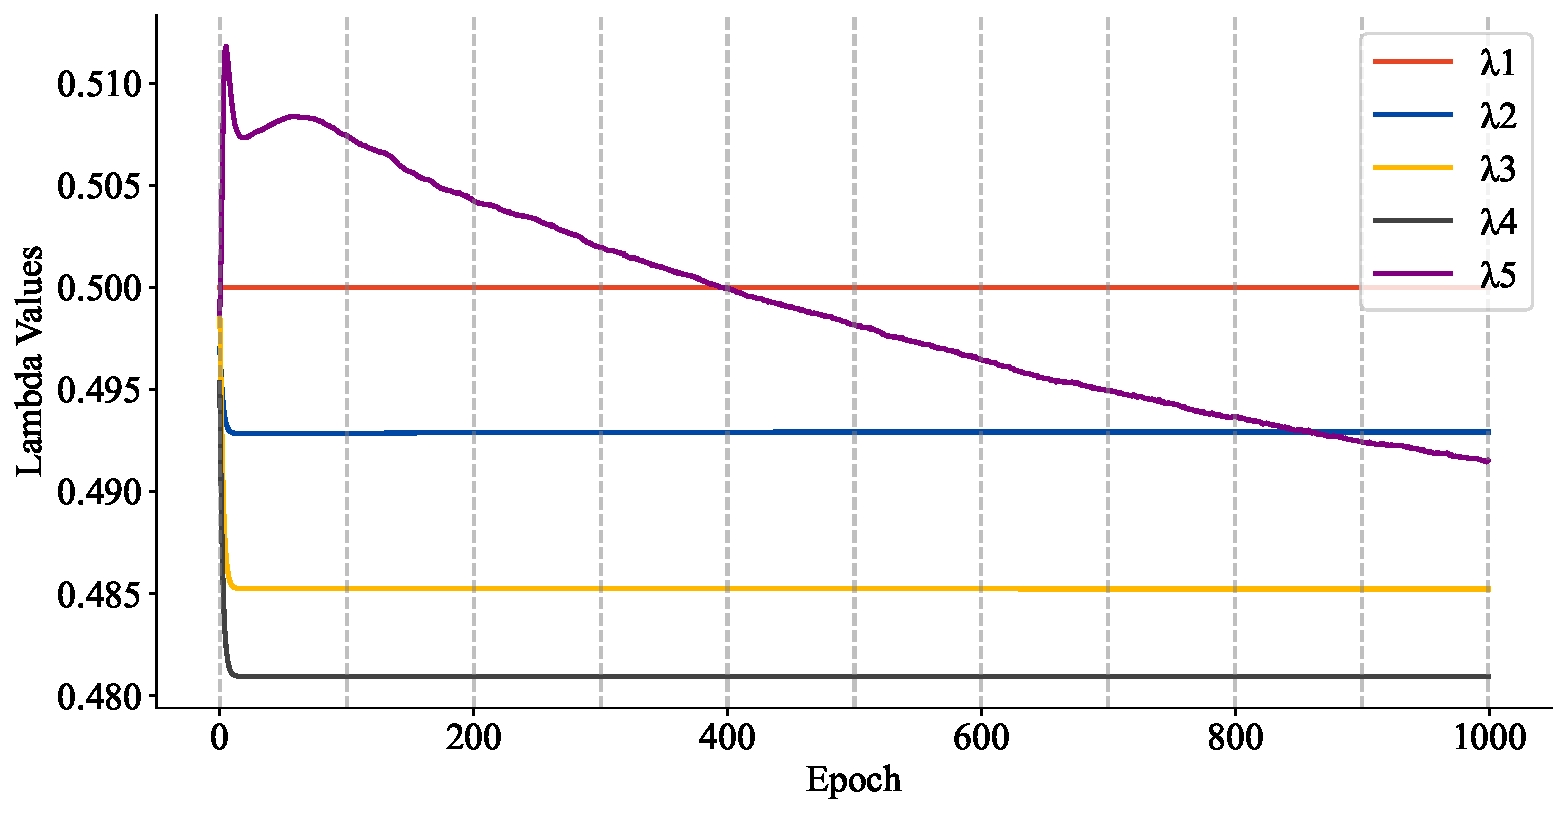
\includegraphics[width=\textwidth]{Figures/lambda_residuals/lambda_values_uracil.pdf}
%         \caption{Uracil}
%     \end{subfigure}
%     \caption{Learned value residuals for MD17 training over 1000 epochs.}
%     \label{fig:lambda_values}
% \end{figure}

% \subsection{Multi-head Output}
% \label{sec:multi_head_output}
% \EScomment{To address the diverse and class-specific dynamics observed across molecules, we employ a multi-head output layer inspired by mixture-of-experts (MoE) architectures \cite{shazeer_outrageously_2017}. Our core idea is to allow our model to dynamically select and combine several expert heads, each specializing in a distinct chemical class, thereby enhancing generalizability across the chemical space.}

% Specifically, given the set of phase space vectors \(\{ \mathbf{z}_1, \dots, \mathbf{z}_N \} = \mathbf{Z} \) of each molecule, we compute the mean pool as:
% \begin{equation}
%     \bar{\mathbf{z}} = \frac{1}{N} \sum\limits_{\mathbf{z} \in \mathbf{Z}} \mathbf{z}.
% \end{equation}
% This global vector is then fed into a softmax-normalized gating network \(\operatorname{HeadGate} \colon \mathbb{R}^d \to \mathbb{R}^{\text{n\_heads}}\), which produces a set of weights, one for each output head:
% \begin{equation}
%     \mathbf{w} = \operatorname{softmax}(\operatorname{HeadGate}(\bar{\mathbf{z}})).
% \end{equation}
% These then weight the contribution of each  \(\operatorname{Project}\) head to the final output:
% \begin{equation*}
%     \mathbf{x}^\dagger = \sum\limits_{i=1}^{\text{n\_heads}} w_i \Big( \operatorname{Project}_i(\mathbf{x}_\text{out}) \Big)
% \end{equation*}
% In the single-task learning case, a single head suffices, and the output reduces to that described in \Cref{sec:project}.

\subsection{Delta-prediction}
\label{sec:delta_prediction}
When delta-prediction is enabled, as in \Cref{fig:MD17_ablation}, we incorporate the initial positions \(\mathbf{x}\) as a residual term, reformulating the model as an operator that learns a displacement field rather than predicting absolute positions. We express this as:
\begin{equation}
    \mathbf{x}^\dagger = \operatorname{Project}(\mathbf{x}_{\text{out}}) + \mathbf{x}.
\end{equation}
Although this approach is implemented in both \gls{egnn} and \gls{egno}, we found it was disabled by default in the codebase of the latter \cite{garcia_satorras_en_2021, xu_equivariant_2024}. Based on empirical results from our ablations, \Cref{fig:MD17_ablation}, we argue there is sufficient evidence to discourage the use of delta-prediction in neural operator-based molecular dynamics simulations.



\section{Further Experiments}
\label{app:further_experiment}
We conduct further experiments on single-task and multitask learning. We consider performance under tail discretization and report results on the RMD17 dataset. For multitask learning, we report performance under random cluster assignment and S2S metrics for the experiments in \Cref{sec:multitask_learning}.

\subsection{Further Single-task Learning Experiments}

\label{app:tail_discretization}
\textbf{MD17 with tail discretization} We find the performance of both \gls{egno} and \gls{atoms} on MD17 with tail discretization remains similar to the performance under uniform discretization discussed in \cref{tab:md17_results}.

\begin{table}[H]
    \centering
    \caption{EGNO and ATOM with final frame sampling. Upper part: S2S \gls{mse}. Lower part: S2T \gls{mse}.}
    \label{tab:md17_finalframe_results}
    \resizebox{\linewidth}{!}{
    \begin{tabular}{lcccccccc}
        \toprule
         & Aspirin & Benzene & Ethanol & Malonaldehyde & Naphthalene & Salicylic & Toluene & Uracil \\
        \midrule
        \gls{egno} & \(9.69{\scriptstyle \pm0.07}\) & \(45.75{\scriptstyle \pm6.28}\) & \(4.56{\scriptstyle \pm0.00}\) & \(\mathbf{12.94}{\scriptstyle \pm0.01}\) & \(0.39{\scriptstyle \pm0.00}\) & \(0.89{\scriptstyle \pm0.01}\) & \(10.99{\scriptstyle \pm0.01}\) & \(0.58{\scriptstyle \pm0.00}\) \\
        \gls{atoms} & \(\mathbf{6.21}{\scriptstyle \pm0.13}\) & \(\mathbf{45.18}{\scriptstyle \pm1.05}\) & \(\mathbf{3.25}{\scriptstyle \pm0.03}\) & \(14.30{\scriptstyle \pm0.26}\) & \(\mathbf{0.38}{\scriptstyle \pm0.00}\) & \(\mathbf{0.81}{\scriptstyle \pm0.00}\) & \(\mathbf{5.51}{\scriptstyle \pm0.13}\) & \(\mathbf{0.54}{\scriptstyle \pm0.00}\) \\
        \midrule
        \rowcolor{gray!20} Gap & \(+35.90\%\) & \(+1.25\%\) & \(+28.78\%\) & \(-10.49\%\) & \(+4.94\%\) & \(+9.78\%\) & \(+49.87\%\) & \(+6.33\%\) \\
        \midrule
        \gls{egno} & \(9.68{\scriptstyle \pm0.07}\) & \(45.85{\scriptstyle \pm6.34}\) & \(4.56{\scriptstyle \pm0.01}\) & \(\mathbf{12.94}{\scriptstyle \pm0.01}\) & \(0.39{\scriptstyle \pm0.00}\) & \(0.89{\scriptstyle \pm0.02}\) & \(10.99{\scriptstyle \pm0.00}\) & \(0.58{\scriptstyle \pm0.00}\) \\
        \gls{atoms} & \(\mathbf{6.22}{\scriptstyle \pm0.14}\) & \(\mathbf{45.16}{\scriptstyle \pm1.05}\) & \(\mathbf{3.25}{\scriptstyle \pm0.03}\) & \(14.31{\scriptstyle \pm0.25}\) & \(\mathbf{0.37}{\scriptstyle \pm0.00}\) & \(\mathbf{0.81}{\scriptstyle \pm0.00}\) & \(\mathbf{5.51}{\scriptstyle \pm0.13}\) & \(\mathbf{0.54}{\scriptstyle \pm0.00}\) \\
        \midrule
        \rowcolor{gray!20} Gap & \(+35.80\%\) & \(+1.52\%\) & \(+28.66\%\) & \(-10.61\%\) & \(+4.97\%\) & \(+10.01\%\) & \(+49.91\%\) & \(+6.34\%\) \\
        \bottomrule
    \end{tabular}
    }
\end{table}


\textbf{Revised MD17 Dataset}
\label{sect:rmd17}
On RMD17, \gls{atoms} reduces the S2S \gls{mse} of \gls{egno} by 19.35\% and the S2T \gls{mse} by 19.89\% on average (\Cref{tab:rmd17_results}), with the largest reductions on toluene, ethanol and paracetamol. \gls{egno} is better only on malonaldehyde. RMD17 stores a random subsample of 100{,}000 frames from each original MD17 trajectory; we sort frames by their original index and only use start frames whose $P$ target frames (at offsets $i\Delta T/P$) are present in the subsample to within 5 frames.
\nopagebreak
\begin{table}[H]
    \centering
    \caption{\gls{mse} (\(\times 10^{-2}\)) of \gls{egno} and \gls{atoms} on RMD17 with uniform sampling. Upper part: S2S \gls{mse}. Lower part: S2T \gls{mse}. Gap is the relative reduction of \gls{atoms} versus \gls{egno}; the last column is the mean gap.}
    \label{tab:rmd17_results}
    \resizebox{\linewidth}{!}{
    \begin{tabular}{lccccccccc}
        \toprule
         & Azobenzene & Ethanol & Malonaldehyde & Naphthalene & Paracetamol & Salicylic & Toluene & Uracil & Mean \\
        \midrule
        \gls{egno} & \(7.33{\scriptstyle \pm0.06}\) & \(4.80{\scriptstyle \pm0.02}\) & \(\mathbf{13.06}{\scriptstyle \pm0.05}\) & \(0.49{\scriptstyle \pm0.00}\) & \(17.13{\scriptstyle \pm0.55}\) & \(0.90{\scriptstyle \pm0.01}\) & \(11.04{\scriptstyle \pm0.35}\) & \(0.62{\scriptstyle \pm0.00}\) & -- \\
        \gls{atoms} & \(\mathbf{6.61}{\scriptstyle \pm0.12}\) & \(\mathbf{3.29}{\scriptstyle \pm0.03}\) & \(13.63{\scriptstyle \pm0.07}\) & \(\mathbf{0.37}{\scriptstyle \pm0.01}\) & \(\mathbf{12.24}{\scriptstyle \pm0.15}\) & \(\mathbf{0.81}{\scriptstyle \pm0.01}\) & \(\mathbf{6.27}{\scriptstyle \pm0.06}\) & \(\mathbf{0.54}{\scriptstyle \pm0.01}\) & -- \\
        \midrule
        \rowcolor{gray!20} Gap & \(+9.88\%\) & \(+31.41\%\) & \(-4.35\%\) & \(+23.91\%\) & \(+28.56\%\) & \(+10.18\%\) & \(+43.19\%\) & \(+11.98\%\) & \(\mathbf{+19.35\%}\) \\
        \midrule
        \gls{egno} & \(6.46{\scriptstyle \pm0.05}\) & \(3.42{\scriptstyle \pm0.02}\) & \(\mathbf{11.32}{\scriptstyle \pm0.02}\) & \(0.43{\scriptstyle \pm0.01}\) & \(13.02{\scriptstyle \pm0.29}\) & \(0.93{\scriptstyle \pm0.02}\) & \(4.85{\scriptstyle \pm0.15}\) & \(0.61{\scriptstyle \pm0.01}\) & -- \\
        \gls{atoms} & \(\mathbf{5.60}{\scriptstyle \pm0.16}\) & \(\mathbf{2.51}{\scriptstyle \pm0.00}\) & \(11.61{\scriptstyle \pm0.06}\) & \(\mathbf{0.36}{\scriptstyle \pm0.00}\) & \(\mathbf{9.98}{\scriptstyle \pm0.07}\) & \(\mathbf{0.67}{\scriptstyle \pm0.01}\) & \(\mathbf{2.87}{\scriptstyle \pm0.03}\) & \(\mathbf{0.52}{\scriptstyle \pm0.01}\) & -- \\
        \midrule
        \rowcolor{gray!20} Gap & \(+13.30\%\) & \(+26.80\%\) & \(-2.54\%\) & \(+15.70\%\) & \(+23.37\%\) & \(+27.61\%\) & \(+40.81\%\) & \(+14.11\%\) & \(\mathbf{+19.89\%}\) \\
        \bottomrule
    \end{tabular}
    }
\end{table}
% \begin{table}[H]
%     \centering
%     \caption{\gls{mse} (\(\times 10^{-2}\)) on RMD17. Upper part: S2S \gls{mse}. Lower part: S2T \gls{mse}}
%     \label{tab:rmd17_results_old}
%     \resizebox{\linewidth}{!}{
%     \begin{tabular}{lccccccccc}
%         \toprule
%         & Azobenzene & Ethanol & Malonaldehyde & Naphthalene & Paracetamol & Salicylic & Toluene & Uracil & Mean \% \\
%         \midrule
%         \gls{egno} & \(10.82{\scriptstyle \pm0.05}\) & \(28.27{\scriptstyle \pm0.16}\) & \(49.25{\scriptstyle \pm0.10}\) & \(1.85{\scriptstyle \pm0.01}\) & \(28.90{\scriptstyle \pm0.20}\) & \(1.26{\scriptstyle \pm0.01}\) & \(28.44{\scriptstyle \pm0.18}\) & \(0.98{\scriptstyle \pm0.01}\) \\
%         \gls{atoms} & \(\mathbf{8.36}{\scriptstyle \pm0.01}\) & \(\mathbf{23.81}{\scriptstyle \pm1.29}\) & \(\mathbf{39.87}{\scriptstyle \pm0.53}\) & \(\mathbf{1.42}{\scriptstyle \pm0.01}\) & \(\mathbf{28.74}{\scriptstyle \pm0.33}\) & \(\mathbf{1.09}{\scriptstyle \pm0.01}\) & \(28.48{\scriptstyle \pm0.02}\) & \(\mathbf{0.89}{\scriptstyle \pm0.01}\) \\
%         \midrule
%         \rowcolor{gray!20} Gap (\%) & \(22.74\%\) & \(15.78\%\) & \(19.05\%\) & \(23.24\%\) & \(0.55\%\) & \(13.49\%\) & \(-0.14\%\) & \(9.18\%\) & \(\mathbf{12.99\%}\) \\
        
%         \midrule
%         \gls{egno} & \(10.75{\scriptstyle \pm0.05}\) & \(28.19{\scriptstyle \pm0.16}\) & \(48.78{\scriptstyle \pm0.10}\) & \(1.80{\scriptstyle \pm0.01}\) & \(\mathbf{28.29}{\scriptstyle \pm0.20}\) & \(1.25{\scriptstyle \pm0.01}\) & \(28.37{\scriptstyle \pm0.18}\) & \(0.98{\scriptstyle \pm0.01}\) \\
%         \gls{atoms} & \(\mathbf{8.61}{\scriptstyle \pm0.01}\) & \(\mathbf{23.48}{\scriptstyle \pm 
%         0.14}\) & \(\mathbf{40.36}{\scriptstyle \pm0.33}\) & \(\mathbf{1.41}{\scriptstyle \pm0.01}\) & \(28.79{\scriptstyle \pm0.33}\) & \(\mathbf{1.08}{\scriptstyle \pm0.01}\) & \(28.45{\scriptstyle \pm0.071}\) & \(\mathbf{0.89}{\scriptstyle \pm0.01}\) \\
%         \midrule
%         \rowcolor{gray!20} Gap (\%) & \(19.91\%\) & \(16.71\%\) & \(17.26\%\) & \(21.67\%\) & \(-1.77\%\) & \(13.60\%\) & \(-0.28\%\) & \(9.18\%\) & \(\mathbf{12.04\%}\) \\
%         \bottomrule
%     \end{tabular}
%     }
% \end{table}

\subsection{Further Multitask Learning Experiments}

\label{sect:random_split}
\textbf{Random-split cross-validation on TG80.} For completeness, we report multitask results under compound-level random cross-validation, where compounds are randomly assigned to the train, validation, and test sets. Relative to the more challenging out-of-domain (UMAP-based) split in \Cref{tab:tg80_umap}, \gls{egno} is comparatively stronger; nevertheless, \gls{atoms} maintains a consistent lead across folds, with mean improvements of 25.10\% on S2S and 25.07\% on S2T.

\begin{table}[H]
  \centering
  \caption{S2S \gls{mse} \((\times10^{-2})\) on TG80 across five random cluster assignments.}
  \resizebox{\linewidth}{!}{%
  \begin{tabular}{llccccc}
    \toprule
     &  & \textbf{Cluster 1} & \textbf{Cluster 2} & \textbf{Cluster 3} & \textbf{Cluster 4} & \textbf{Cluster 5} \\
     \midrule
    \multirow{2}{*}{OOD}
       & \gls{egno} & \(71.83{\scriptstyle \pm0.00}\) & \(76.92{\scriptstyle \pm0.00}\) & \(68.99{\scriptstyle \pm0.00}\) & \(101.27{\scriptstyle \pm0.00}\) & \(83.20{\scriptstyle \pm0.00}\) \\
       & \gls{atoms} & \(\mathbf{56.88}{\scriptstyle \pm0.88}\) & \(\mathbf{59.34}{\scriptstyle \pm0.98}\) & \(\mathbf{54.78}{\scriptstyle \pm1.54}\) & \(\mathbf{67.23}{\scriptstyle \pm6.88}\) & \(\mathbf{60.22}{\scriptstyle \pm2.19}\) \\
      \cmidrule(lr){2-7}
      \rowcolor{gray!20} & Gap & \(+20.81\%\) & \(+22.85\%\) & \(+20.60\%\) & \(+33.62\%\) & \(+27.63\%\) \\
    \bottomrule
  \end{tabular}
  }
  \label{tab:tg80_random_s2s}
\end{table}

\begin{table}[H]
  \centering
  \caption{S2T \gls{mse} \((\times10^{-2})\) on TG80 across five random cluster assignments.}
  \resizebox{\linewidth}{!}{%
  \begin{tabular}{llccccc}
    \toprule
     &  & \textbf{Cluster 1} & \textbf{Cluster 2} & \textbf{Cluster 3} & \textbf{Cluster 4} & \textbf{Cluster 5} \\
     \midrule
    \multirow{2}{*}{OOD}
       & \gls{egno} & \(63.23{\scriptstyle \pm0.00}\) & \(64.49{\scriptstyle \pm0.00}\) & \(59.18{\scriptstyle \pm0.00}\) & \(85.87{\scriptstyle \pm0.00}\) & \(69.46{\scriptstyle \pm0.00}\) \\
       & \gls{atoms} & \(\mathbf{48.61}{\scriptstyle \pm1.89}\) & \(\mathbf{50.96}{\scriptstyle \pm1.34}\) & \(\mathbf{46.54}{\scriptstyle \pm1.36}\) & \(\mathbf{57.72}{\scriptstyle \pm7.32}\) & \(\mathbf{50.66}{\scriptstyle \pm2.14}\) \\
      \cmidrule(lr){2-7}
      \rowcolor{gray!20} & Gap & \(+23.13\%\) & \(+20.99\%\) & \(+21.37\%\) & \(+32.79\%\) & \(+27.07\%\) \\
    \bottomrule
  \end{tabular}
  }
  \label{tab:tg80_random_s2t}
\end{table}


\textbf{Multitask S2S results on TG80 under UMAP cluster cross-validation.} The S2S side of the multitask learning results follow closely from their S2T counterparts presented in \Cref{sec:multitask_learning}.
\label{app:s2s_result}

\begin{table}[H]
  \centering
  \caption{S2S \gls{mse} \((\times10^{-2})\) on TG80 across five UMAP cluster assignments. Gap is the relative reduction of \gls{atoms} versus \gls{egno}.}
  \resizebox{\linewidth}{!}{%
  \begin{tabular}{llccccc}
    \toprule
     &  & \textbf{Cluster 1} & \textbf{Cluster 2} & \textbf{Cluster 3} & \textbf{Cluster 4} & \textbf{Cluster 5} \\
     \midrule
     \multirow{3}{*}{ID}
      & \gls{egno}  & \(51.83{\scriptstyle \pm0.79}\) & \(103.99{\scriptstyle \pm0.22}\) & \(143.61{\scriptstyle \pm0.84}\) & \(154.75{\scriptstyle \pm0.60}\) & \(109.30{\scriptstyle \pm0.33}\) \\
      & \gls{atoms} & \(\mathbf{6.18}{\scriptstyle \pm0.25}\) & \(\mathbf{9.05}{\scriptstyle \pm0.35}\) & \(\mathbf{5.95}{\scriptstyle \pm0.16}\) & \(\mathbf{5.08}{\scriptstyle \pm0.45}\) & \(\mathbf{6.18}{\scriptstyle \pm0.41}\) \\
      \cmidrule(lr){2-7}
      \rowcolor{gray!20} & Gap (\%) & \(88.08\%\) & \(91.30\%\) & \(95.86\%\) & \(96.72\%\) & \(94.34\%\) \\
    \midrule
    \multirow{4}{*}{OOD}
      & \gls{egno}  & \(53.19{\scriptstyle \pm0.96}\) & \(1788.34{\scriptstyle \pm2874.88}\) & \(149.38{\scriptstyle \pm1.55}\) & \(163.23{\scriptstyle \pm0.40}\) & \(112.36{\scriptstyle \pm1.70}\) \\
      & EGNN\text{-}S & \(52.46{\scriptstyle \pm0.43}\) & \(59210.80{\scriptstyle \pm52351.92}\) & \(150.22{\scriptstyle \pm1.10}\) & \(2965.22{\scriptstyle \pm4852.19}\) & \(111.18{\scriptstyle \pm0.57}\) \\
      & EGNN\text{-}R & \(52.11{\scriptstyle \pm0.93}\) & \(116.96{\scriptstyle \pm0.68}\) & \(151.26{\scriptstyle \pm2.45}\) & \(163.20{\scriptstyle \pm0.27}\) & \(110.88{\scriptstyle \pm1.90}\) \\
      & \gls{atoms} & \(\mathbf{42.75}{\scriptstyle \pm0.31}\) & \(\mathbf{72.22}{\scriptstyle \pm5.54}\) & \(\mathbf{86.26}{\scriptstyle \pm7.00}\) & \(\mathbf{97.83}{\scriptstyle \pm7.30}\) & \(\mathbf{63.71}{\scriptstyle \pm4.79}\) \\
      \cmidrule(lr){2-7}
      \rowcolor{gray!20} & Gap (\%) & \(19.62\%\) & \(95.96\%\) & \(42.25\%\) & \(40.07\%\) & \(43.30\%\) \\
    \bottomrule
  \end{tabular}
  }
  \label{tab:tg80_umap_s2s}
\end{table}

\newpage

\begin{wraptable}{r}{0.42\textwidth}
    \centering
    \caption{\gls{mse} \((\times10^{-2})\) on full-dataset TG80 \gls{atoms} and single-task \gls{atoms}. S2S upper, S2T lower.}
    \begin{tabular}{lc}
        \toprule
        & Formic Acid \\
        \midrule
        Single-task \gls{atoms} & \textbf{26.51} \\
        All-data \gls{atoms} & 29.37 \\
        \midrule
        \rowcolor{gray!20} Gap (\%) & \(-10.79\%\) \\
        \midrule
        Single-task \gls{atoms} & \textbf{17.80} \\
        All-data \gls{atoms} & 19.92 \\
        \midrule
        \rowcolor{gray!20} Gap (\%) & \(-11.91\%\) \\
        \bottomrule
    \end{tabular}
    \label{tab:placeholder}
    \vspace{-0.5\baselineskip}
\end{wraptable}
\textbf{Multitask S2S Versus Single Task} We evaluate a multitask \gls{atoms} model trained on all available trajectories, pooling both ID and OOD clusters, against a single-task \gls{atoms} trained separately on each compound. On formic acid, the multitask model comes within 12\% of the single-task model on both S2S and S2T \gls{mse}, while also covering every other compound in TG80.

% \begin{table}[H]
%     \centering
%     \caption{\gls{mse} \((\times10^{-2})\) on full-dataset TG80 \gls{atoms} and single-task \gls{atoms}. S2S upper, S2T lower.}
%     \begin{tabular}{lc}
%         \toprule
%         & Formic Acid \\
%         \midrule
%         Single-task \gls{atoms} & 26.40 \\
%         All-data \gls{atoms} & \textbf{22.39} \\
%         \midrule
%         \rowcolor{gray!20} Gap (\%) & \(15.19\%\) \\
%         \midrule
%         Single-task \gls{atoms} & \textbf{18.10} \\
%         All-data \gls{atoms} & 18.72 \\
%         \midrule
%         \rowcolor{gray!20} Gap (\%) & \(-3.43\%\) \\
%         \bottomrule
%     \end{tabular}
%     \label{tab:placeholder}
% \end{table}

% in text

\subsection[Monte Carlo Estimation of Quasi-equivariance]{Monte Carlo Estimation of\\ Quasi-equivariance}
\label{app:quasi_equivariance_mc}
{For both the pretrained \gls{atoms} and the non-equivariant lifting variant, we estimate the quantity in \Cref{def:quasi_equivariance} by Monte Carlo, drawing \(N\) test states \(x_n\) and, for each, \(R\) rotations \(g_{n,r}\) sampled uniformly (Haar) from \(\mathrm{SO}(3)\). We approximate
\begin{equation*}
    \varepsilon \approx \frac{1}{N R} \sum_{n=1}^{N} \sum_{r=1}^{R}
    \left\|
            f\bigl(\phi(g_{n,r})(x_n)\bigr)
            - \rho(g_{n,r})\bigl(f(x_n)\bigr)
    \right\|_2 ,
\end{equation*}
where the norm is taken over the Cartesian coordinates of each predicted atom position and the result is averaged over atoms and predicted timesteps.
We report our estimates of \(\varepsilon\) for various \gls{atoms} models trained on MD17 single task learning in \Cref{tab:equivariance_defect}. \gls{atoms} shows a lower equivariance defect than the non-equivariant variant on aspirin, malonaldehyde and toluene, with the largest reduction on toluene (\(2.2\times\)); on ethanol, naphthalene, salicylic acid and uracil the non-equivariant variant has the lower defect.
}

\begin{table}[H]
%— Top: Full‐width big table —
\centering
\caption{Estimates of the equivariance defect \(\varepsilon\) \((\times10^{-2}\)~\AA{}) via Monte Carlo over 20 Haar-random rotations and 10 test batches with 2SD intervals.}
\label{tab:equivariance_defect}
\resizebox{\linewidth}{!}{%
    \begin{tabular}{lccccccc}
        \toprule
         & Aspirin & Ethanol & Malonaldehyde & Naphthalene & Salicylic & Toluene & Uracil \\
        \midrule 
        Non-equivariant \gls{atoms} & \(137.72{\scriptstyle \pm85.15}\) & \(\mathbf{35.48}{\scriptstyle \pm18.91}\) & \(57.55{\scriptstyle \pm32.70}\) & \(\mathbf{88.66}{\scriptstyle \pm41.67}\) & \(\mathbf{119.18}{\scriptstyle \pm64.44}\) & \(3750.90{\scriptstyle \pm3815.93}\) & \(\mathbf{108.73}{\scriptstyle \pm78.73}\) \\

        \textbf{\gls{atoms}} & \(\mathbf{130.09}{\scriptstyle \pm95.67}\) & \(37.47{\scriptstyle \pm22.68}\) & \(\mathbf{52.25}{\scriptstyle \pm31.70}\) & \(204.68{\scriptstyle \pm174.68}\) & \(259.44{\scriptstyle \pm188.28}\) & \(\mathbf{1710.83}{\scriptstyle \pm1868.94}\) & \(229.57{\scriptstyle \pm228.08}\) \\
        \bottomrule
    \end{tabular}
}
\end{table}



% \subsection{Explicit Hydrogen Representation}
% We hypothesized that our model's underperformance relative to \gls{egno} in predicting malonaldehyde was due to the omission of explicit hydrogens, which limits its ability to capture electron delocalization effects involving hydroxyl hydrogens. We tested two explicit hydrogen methods: 
% \begin{enumerate}
%     \item Including all hydrogens with gradients computed for all atoms during training
%     \item Including all hydrogens but computing gradients only for heavy atoms
% \end{enumerate}

% Contrary to conventional \gls{md} practice, neither method improved heavy-atom test loss.

% \begin{table}[H]
%     \centering
%     \caption{\gls{atoms} MD17 S2T MSE with implicit hydrogens (\gls{atoms} baseline) and two explicit hydrogen approaches.}
%     \label{tab:explicit_hydrogens}
%     \begin{tabular}{lcc}
%         \toprule
%         & Aspirin & Malonaldehyde \\
%         \midrule
%         Explicit hydrogens 1 & \(7.48{\scriptstyle \pm0.11}\) & \(15.15{\scriptstyle \pm0.22}\) \\
%         Explicit hydrogens 2 & \(6.96{\scriptstyle \pm0.20}\) & \(13.52{\scriptstyle \pm0.10}\)\\
%         Implicit hydrogens & \(6.52{\scriptstyle \pm0.08}\) & \(13.51{\scriptstyle \pm0.10}\) \\
%         \bottomrule
%     \end{tabular}
% \end{table}

% \subsection{Varying T-RoPE Base}
% We experimented with several \gls{trope} bases, but found no difference in performance at either \(P=8\) pr \(P=32\). Our results are available in \Cref{tab:trope_bases}.
% \begin{table}[H]
%     \centering
%     \caption{S2T \gls{mse} across varying \gls{trope} bases and \(P\).}
%     \label{tab:trope_bases}
%     \begin{tabular}{lcc}
%         \toprule
%         Base & \(P=8\) & \(P=16\) \\
%         \midrule
%         100 & \(5.41{\scriptstyle \pm0.13}\) & \(5.41{\scriptstyle \pm0.13}\) \\
%         1000 & \(5.61{\scriptstyle \pm0.04}\) & \(5.38{\scriptstyle \pm0.31}\) \\
%         10\,000 & \(5.57{\scriptstyle \pm0.04}\) & \(5.39{\scriptstyle \pm0.05}\) \\
%         100\,000 & \(5.69{\scriptstyle \pm0.13}\) & \(5.52{\scriptstyle \pm0.26}\) \\
%         \bottomrule
%     \end{tabular}
% \end{table}

\section{Experimental Details}
\label{sect:details}

\subsection{Software and Hardware Details}
All experiments were conducted using Python 3.12, NumPy 2.2.1 \cite{harris_array_2020}, PyTorch 2.5.1 \cite{paszke_pytorch_2019}, e3nn 0.5.6 \cite{geiger_e3nn_2022} and PyTorch Optimizer 3.5.0 \cite{kim_pytorch_optimizer_2021}. We use RDKit 2024.9.6 \cite{greg_landrum_rdkitrdkit_2025} and PubChemPy 1.0.4 to construct TG80. All single-task training was performed on an NVIDIA RTX 5080 (16 GB) with CUDA 12.4, running on Ubuntu 24.04. {We use Ase 3.26.0 \cite{larsen_atomic_2017} and MACE-Torch 0.3.14 \cite{kovacs_mace-off_2025} in the experiments of \Cref{app:inference_times}.}

\subsection{Training Times and Compute Requirements}
\label{sec:model_compute_time}
\textbf{Single-task training time} We roughly wall-clock normalised our \gls{atoms} and \gls{egno} parameter counts, resulting in respective learnable parameter counts of 910\,320 and 335\,770.

\begin{table}[H]
    \centering
    \caption{Compute cost of single-task training on all RMD17 molecules over 1000 epochs. Both \gls{atoms} (910\,320 params) and \gls{egno} (335\,770 params) are under \texttt{torch.compile} on a Titan V. Total FLOPS is wall-clock time multiplied by the peak FP32 throughput of the GPU.}
    \label{tab:md17_compute_cost}
    \resizebox{\linewidth}{!}{%
    \begin{tabular}{llcccccccc}
            \toprule
            Model & Metric & Azobenzene & Ethanol & Malonaldehyde & Naphthalene & Paracetamol & Salicylic & Toluene & Uracil \\
            \midrule
            \multirow{3}{*}{\gls{egno}}
             & Time (mins) & \(4.09\pm\scriptstyle{0.15}\) & \(3.62\pm\scriptstyle{0.42}\) & \(3.65\pm\scriptstyle{0.01}\) & \(5.01\pm\scriptstyle{0.02}\) & \(9.02\pm\scriptstyle{1.22}\) & \(5.16\pm\scriptstyle{0.03}\) & \(3.93\pm\scriptstyle{0.02}\) & \(4.35\pm\scriptstyle{0.04}\) \\
             & Total FLOPS (\(\times 10^{12}\)) & \(3681.24\) & \(3257.70\) & \(3282.09\) & \(4513.37\) & \(8114.44\) & \(4641.50\) & \(3539.92\) & \(3915.98\) \\
             & Epochs/min & \(244.48\) & \(276.27\) & \(274.22\) & \(199.41\) & \(110.91\) & \(193.90\) & \(254.24\) & \(229.83\) \\
            \midrule
            \multirow{3}{*}{\gls{atoms}}
             & Time (mins) & \(5.81\pm\scriptstyle{0.02}\) & \(5.79\pm\scriptstyle{0.06}\) & \(5.79\pm\scriptstyle{0.00}\) & \(5.86\pm\scriptstyle{0.01}\) & \(5.89\pm\scriptstyle{0.02}\) & \(5.85\pm\scriptstyle{0.01}\) & \(5.81\pm\scriptstyle{0.01}\) & \(5.83\pm\scriptstyle{0.02}\) \\
             & Total FLOPS (\(\times 10^{12}\)) & \(5226.49\) & \(5212.53\) & \(5213.50\) & \(5271.19\) & \(5297.84\) & \(5263.76\) & \(5224.91\) & \(5247.33\) \\
             & Epochs/min & \(172.20\) & \(172.66\) & \(172.63\) & \(170.74\) & \(169.88\) & \(170.98\) & \(172.25\) & \(171.52\) \\
            \midrule
            \rowcolor{gray!20}
            \multicolumn{2}{c}{Total FLOPS Reduction (\%)}  & \(-41.98\%\) & \(-60.01\%\) & \(-58.85\%\) & \(-16.79\%\) & \(+34.71\%\) & \(-13.41\%\) & \(-47.60\%\) & \(-34.00\%\) \\
            \bottomrule
        \end{tabular}
    }
\end{table}

\textbf{Multitask training time} In multitask training on TG80, our upsized \gls{atoms} model contained 4\,347\,428 parameters, compared to 335\,770 for \gls{egno}. Despite this, \gls{atoms} only trained between 5\% and 30\% slower than \gls{egno}. This is perhaps unsurprising given the much higher FLOPS-utilization of the transformer architecture upon which \gls{atoms} is based.

\begin{table}[H]
    \centering
    \caption{Compute cost of multitask training on the five TG80 cluster splits over 1000 epochs. Both \gls{atoms} (4\,347\,428 params) and \gls{egno} (335\,770 params) are under \texttt{torch.compile} on a Titan V. Total FLOPS is wall-clock time multiplied by the peak FP32 throughput of the GPU.}
    \label{tab:tg80_compute_cost}
    \resizebox{\linewidth}{!}{%
    \begin{tabular}{llccccc}
            \toprule
            Model &  & Fold1 & Fold2 & Fold3 & Fold4 & Fold5 \\
            \midrule
            \multirow{3}{*}{\gls{egno}} & Time (mins) & \(9.61{\scriptstyle \pm1.21}\) & \(8.56{\scriptstyle \pm0.06}\) & \(9.04{\scriptstyle \pm0.11}\) & \(9.31{\scriptstyle \pm0.20}\) & \(8.98{\scriptstyle \pm0.01}\) \\
             & Total FLOPS ($\times10^{12}$) & 8645.66 & 7703.33 & 8136.98 & 8378.06 & 8084.98 \\
             & Epochs/min & \(104.10\) & \(116.83\) & \(110.61\) & \(107.42\) & \(111.32\) \\
            \midrule
            \multirow{3}{*}{\gls{atoms}} & Time (mins) & \(10.16{\scriptstyle \pm0.49}\) & \(10.55{\scriptstyle \pm0.02}\) & \(11.62{\scriptstyle \pm0.41}\) & \(12.38{\scriptstyle \pm0.12}\) & \(10.39{\scriptstyle \pm0.41}\) \\
             & Total FLOPS ($\times10^{12}$) & 9140.57 & 9497.79 & 10455.34 & 11141.73 & 9355.37 \\
             & Epochs/min & \(98.46\) & \(94.76\) & \(86.08\) & \(80.78\) & \(96.20\) \\
            \midrule
            \rowcolor{gray!20}
            \multicolumn{2}{c}{Total FLOPS Reduction (\%)}  & \(-5.72\%\) & \(-23.29\%\) & \(-28.49\%\) & \(-32.99\%\) & \(-15.71\%\) \\
            \bottomrule
        \end{tabular}
    }
\end{table}
\subsection{Inference Times}
\label{app:inference_times}
{We compare inference times on MD17 and MD22 across \gls{atoms}, the pretrained machine learning interaction potential MACE-OFF24 (Medium) \cite{kovacs_mace-off_2025}, and the classical Lennard-Jones potential \cite{larsen_atomic_2017, schwerdtfeger_100_2024} and the molecular forcefield. We report inference times in seconds with 2SD intervals. We exclude AMBER results on Uracil as we were unable to run simulations for this molecule \cite{case_ambertools_2023}.}

\begin{table}[H]
    \centering
    \caption{Seconds to produce timestep \(\Delta T = 3000\) of each MD17 trajectory at \texttt{float32} precision.}
    \label{tab:inference_md17}
    \resizebox{\linewidth}{!}{%
        \begin{tabular}{llrrrrrrr}
            \toprule
             &  & Aspirin & Ethanol & Malonaldehyde & Naphthalene & Salicylic & Toluene & Uracil \\
            \midrule 
            \multirow{4}{*}{\(\Delta T = 3000\)} 
              &  MACE-OFF
              & \(42.605\pm\scriptstyle{3.945}\) 
              & \(39.656\pm\scriptstyle{0.568}\) 
              & \(39.782\pm\scriptstyle{0.141}\) 
              & \(39.916\pm\scriptstyle{0.155}\) 
              & \(39.620\pm\scriptstyle{0.030}\) 
              & \(40.271\pm\scriptstyle{2.851}\) 
              & \(40.166\pm\scriptstyle{0.902}\) \\
              &  AMBER
              & \(37.746\pm\scriptstyle{0.536}\) 
              & \(38.512\pm\scriptstyle{1.243}\) 
              & \(36.806\pm\scriptstyle{0.194}\) 
              & \(38.512\pm\scriptstyle{1.243}\) 
              & \(37.621\pm\scriptstyle{1.412}\) 
              & \(38.061\pm\scriptstyle{0.848}\) 
              & \(-\) \\
            
              & Lennard-Jones
              & \(2.499\pm\scriptstyle{0.266}\) 
              & \(1.604\pm\scriptstyle{0.208}\) 
              & \(1.529\pm\scriptstyle{0.039}\) 
              & \(2.174\pm\scriptstyle{0.094}\) 
              & \(1.981\pm\scriptstyle{0.011}\) 
              & \(1.906\pm\scriptstyle{0.006}\) 
              & \(1.804\pm\scriptstyle{0.196}\) \\
    
              & \gls{atoms}
              & \(0.849\pm\scriptstyle{0.926}\) 
              & \(0.259\pm\scriptstyle{0.097}\) 
              & \(0.714\pm\scriptstyle{0.241}\) 
              & \(0.467\pm\scriptstyle{0.149}\) 
              & \(0.450\pm\scriptstyle{0.090}\) 
              & \(0.341\pm\scriptstyle{0.075}\) 
              & \(0.373\pm\scriptstyle{0.076}\) \\
              \midrule
            \multirow{3}{*}{\(\Delta T = 10\ 000\)} 
              & MACE-OFF
              & \(143.413\pm\scriptstyle{3.313}\) 
              & \(142.569\pm\scriptstyle{5.584}\) 
              & \(136.380\pm\scriptstyle{3.964}\) 
              & \(140.288\pm\scriptstyle{9.136}\) 
              & \(140.103\pm\scriptstyle{3.398}\) 
              & \(140.372\pm\scriptstyle{4.754}\) 
              & \(141.598\pm\scriptstyle{1.020}\) \\
              
              &   AMBER
              & \(133.900\pm\scriptstyle{3.815}\) 
              & \(128.385\pm\scriptstyle{3.812}\) 
              & \(121.095\pm\scriptstyle{0.968}\) 
              & \(121.607\pm\scriptstyle{1.195}\) 
              & \(120.319\pm\scriptstyle{1.591}\) 
              & \(120.800\pm\scriptstyle{0.398}\) 
              & \(-\) \\
            
              & Lennard-Jones
              & \(7.797\pm\scriptstyle{0.369}\) 
              & \(5.533\pm\scriptstyle{0.425}\) 
              & \(5.167\pm\scriptstyle{0.221}\) 
              & \(7.453\pm\scriptstyle{0.376}\) 
              & \(6.721\pm\scriptstyle{0.418}\) 
              & \(6.477\pm\scriptstyle{0.204}\) 
              & \(5.921\pm\scriptstyle{0.522}\) \\
    
              & \gls{atoms}
              & \(2.554\pm\scriptstyle{0.945}\) 
              & \(1.002\pm\scriptstyle{0.184}\) 
              & \(1.634\pm\scriptstyle{0.200}\) 
              & \(1.098\pm\scriptstyle{0.209}\) 
              & \(1.116\pm\scriptstyle{0.083}\) 
              & \(0.964\pm\scriptstyle{0.185}\) 
              & \(0.990\pm\scriptstyle{0.171}\) \\
            \bottomrule
        \end{tabular}
    }
\end{table}

\begin{table}[H]
    %— Top: Full‐width big table —
    \centering
    \caption{Seconds to produce timestep \(\Delta T = 3000\) of each MD22 trajectory at \texttt{float32} precision.}
    \label{tab:inference_md22}
        \begin{tabular}{lrrr}
            \toprule
             & Ac-Ala3-NHME & DHA & Stachyose \\
            \midrule 
            MACE-OFF & \(44.737\pm\scriptstyle{4.615}\) & \(42.042\pm\scriptstyle{0.720}\) & \(47.913\pm\scriptstyle{0.546}\) \\
            
            Lennard-Jones & \(4.700\pm\scriptstyle{0.212}\) & \(3.790\pm\scriptstyle{0.246}\) & \(6.613\pm\scriptstyle{0.147}\) \\
    
            \gls{atoms} & \(1.302\pm\scriptstyle{0.766}\) & \(0.914\pm\scriptstyle{0.055}\) & \(3.075\pm\scriptstyle{0.080}\) \\
            \bottomrule
        \end{tabular}
\end{table}

% \begin{table}[H]
%     \centering
%     \caption{Minutes to complete 100 epochs on MD17.}
%     \label{tab:MD17_times}
%     \resizebox{\linewidth}{!}{
%     \begin{tabular}{lccccccc}
%         \toprule
%         & Uracil & Nitrobenzene & Naphthalene & Indole & Butanol & Mean \\
%         \midrule
%         \gls{egno} & \( 31.29{\scriptstyle \pm16.34} \) & \( 33.33{\scriptstyle \pm11.17} \) & \( 32.19{\scriptstyle \pm10.76} \) & \( 64.61{\scriptstyle \pm12.56} \) & \( 68.13{\scriptstyle \pm0.67} \) & \( 44.32{\scriptstyle \pm20.14} \) \\
%         \gls{atoms} & \( 3.06{\scriptstyle \pm0.43} \) & \( 7.75{\scriptstyle \pm0.18} \) & \( 3.59{\scriptstyle \pm0.41} \) & \( 3.19{\scriptstyle \pm0.18} \) & \( 5.15{\scriptstyle \pm0.18} \)
%     \end{tabular}
%     }
% \end{table}
\newpage
\subsection{ATOM Hyperparameters}
\label{appx:my_hyperparams}
We employ the same dataset splitting and discretization parameters reported in \textcite{xu_equivariant_2024} for the MD17. We set the batch size to \(192\), train for 1000 epochs, use the AdamW-AMSGrad optimizer \cite{loshchilov_decoupled_2017} with an \(\epsilon\) of \(1\times10^{-10}\) to avoid instability associated with the small gradients produced by zero-initialised weight matrices in early training \cite{jordan_nanogpt_2025}. For TG80 (single- and multitask), we train for 50 epochs without noise augmentation, sample the horizon \(\Delta T\) log-uniformly from \([8, 24\,000]\) frames, and employ the Muon optimizer \cite{jordan_muon_2024, kim_pytorch_optimizer_2021}. We present a complete overview of our hyperparameters in \Cref{tab:atom_hparams}. For MD17 malonaldehyde we use seven layers, embedding dimension 512, learning rate \(4\times10^{-4}\), input noise \(\sigma=0.15\) and delta (residual) position updates. On MD22 we use batch size 100 and \(\beta_1=0.9\); for stachyose we use seven layers, batch size 64, learning rate \(3.5\times10^{-4}\), 250 epochs and input noise \(\sigma=0.05\).

\begin{table}[h]
    \centering
    \caption{Hyperparameters for \gls{atoms}. MD17 hyperparameters are shared across all molecules unless otherwise noted.}
    \label{tab:atom_hparams}
    \resizebox{\linewidth}{!}{
    \begin{tabular}{cccc}
        Module & & MD17, RMD17 & TG80 (single- and multitask) \\
        % Module & & MD17, RMD17 Value & \(N\)-body Value & Multitask \\
        \midrule
        Training & & \\
        & Batch size & \( 192 \) & \( 192 \) \\
        & Epochs & \( 1000 \) & \(50\) \\
        & Max grad norm & \( 1.0 \) & \(1.0\) \\
        & Input noise \(\sigma\) & \( 0.1 \) & \(0\) \\
        & \(\Delta T\) & \( 3000 \) & \( \mathrm{LogUnif}[8, 24\,000] \) \\
        & Timesteps \(P\) & \( 8 \) & \( 8 \) \\
        & Train/Val/Test & \( (500,2\,000,2\,000) \) & \( (6\,500,13\,000,13\,000) \) \\
        & \gls{rwpe} length & 0 (unused) & 8 \\
        \midrule
        Optimiser & & \\
        & Optimiser type & AdamW-AMSGrad & Muon  \\
        & Learning rate & \( 1\times10^{-3} \) & \( 2\times10^{-3} \) \\
        & \(\beta_1, \beta_2\) & \( (0.95, 0.999) \) & \( (0.95, 0.999) \) \\
        & Weight decay & \( 1\times10^{-5} \) & \( 1\times10^{-5} \) \\
        & \(\epsilon\) & \( 1\times10^{-10} \) & \( 1\times10^{-10} \) \\
        \midrule
        Model & & \\
        & Embedding dim & \( 256 \) & \( 256 \) \\
        & No. layers & \( 6 \) & \( 6 \) \\
        & No. attention heads & \( 8 \) & \( 8 \) \\
        & No. output heads & \(1\) & \(1\) \\
        & Attention dropout & \( 0.2 \) & \( 0.2 \) \\
        & RoPE frequency & \( 1000 \) & \( 1000 \)\\
        & T-RoPE \(\tau\) & \( 375 \) & \( 375 \)\\
        & MLP layers & \( 2 \) & \( 2 \) \\
        & MLP activation & SwiGLU & SwiGLU \\
        & MLP dropout & \( 0.0 \) & \( 0.0 \) \\
        & Norm type & RMS norm & RMS norm \\
        & Learnable value residuals & True & True \\
        \bottomrule
    \end{tabular}}
\end{table}
\newpage
\subsection{EGNO Hyperparameters and Experimental Details}
\label{appx:egno_hyperparams}
We generated the \gls{egno} results reported in \Cref{tab:md17_results} with the same discretization parameters and hyperparameters as used in their experiments. We reduce the number of epochs from \(10\ 000\) to \(1\ 000\), use a batch size of 100 with the AdamW-AMSGrad optimizer \cite{loshchilov_decoupled_2017}, and select the best validation loss epoch for testing. On TG80, we train for 50 epochs with batch size 192, sample \(\Delta T\) log-uniformly from \([3\,000, 24\,000]\) frames, and employ the Muon optimizer \cite{jordan_muon_2024, kim_pytorch_optimizer_2021}. Complete hyperparameters are displayed in \Cref{tab:egno_hparams}.

\begin{table}[H]
    \centering
    \caption{Hyperparameter values for \gls{egno} across each benchmark dataset.}
    \label{tab:egno_hparams}
    \resizebox{\linewidth}{!}{
    \begin{tabular}{cccc}
        Module & & MD17, RMD17 & TG80 (single- and multitask) \\
        \midrule
        Training & & \\
        & Batch size & \( 100 \) & \( 192 \) \\
        & Epochs & \( 1000 \) & \( 50 \) \\
        & Max grad norm & \( 1.0 \) & \( 1.0 \) \\
        & Input noise \(\sigma\) & \( 0 \) & \(0\) \\
        & \(\Delta T\) & \( 3000 \) & \( \mathrm{LogUnif}[3\,000, 24\,000] \) \\
        & Timesteps \(P\) & \( 8 \) & \(8\) \\
        & Train/Val/Test & \( (500,2\,000,2\,000) \) & \( (6\,500,13\,000,13\,000) \) \\
        & \gls{rwpe} length & 8 & 8 \\
        \midrule
        Optimiser & & \\
        & Optimiser type & AdamW-AMSGrad & Muon \\
        & Learning rate & \( 1\times10^{-3} \) & \( 2\times10^{-3} \) \\
        & \(\beta_1, \beta_2\) & \( (0.9, 0.999) \) & \( (0.95, 0.999) \) \\
        & Weight decay & \( 1\times10^{-5} \) & \( 1\times10^{-5} \) \\
        & \(\epsilon\) & \( 1\times10^{-10} \) & \( 1\times10^{-10} \) \\
        \midrule
        Scheduler & & \\
        & Scheduler type & None & None \\
        \midrule
        Model & & \\
        & Embedding dim & \( 64 \) & \( 64 \) \\
        & No. \gls{egno} layers & \( 5 \) & \( 5 \) \\
        & Temporal convolution activation & LeakyRELU & LeakyRELU \\
        & MLP layers & \( 2 \) & \( 2 \) \\
        & MLP activation & SiLU & SiLU \\
        & MLP dropout & \( 0 \) & \( 0 \) \\
        & Time embedding dim & 32 & 32 \\
        & Fourier modes & 2 & 2 \\
        \bottomrule
    \end{tabular}}
\end{table}

\newpage
\section{Propositions and Proofs}
% \subsection{Tensor Product Equivariance}
% \label{appx:tpeq}
% \newtheorem{tpeq}{Tensor product equivariance}
% \begin{tpeq} \label{thm:tpeq}
%     Let \( G \) be a group acting on \( \mathbb{R}^n \), and let \( V \) and \( W \) be vector spaces equipped with representations \( \rho: G \to GL(V) \) and \( \sigma: G \to GL(W) \), respectively. Suppose \( f: \mathbb{R}^n \to V \) and \( g: \mathbb{R}^n \to W \) are equivariant functions satisfying:
%     \[
%     f(h \cdot x) = \rho(h) f(x), \quad g(h \cdot x) = \sigma(h) g(x), \quad \forall h \in G.
%     \]
%     Then, their tensor product function
%     \[
%     (f \otimes g)(x) = f(x) \otimes g(x)
%     \]
%     is equivariant under the tensor product representation \( \rho \otimes \sigma \), i.e.,
%     \[
%     (f \otimes g)(h \cdot x) = (\rho \otimes \sigma)(h) (f(x) \otimes g(x)).
%     \]
% \end{tpeq}

% \begin{proof}
%     Applying \( h \in G \) to the input \( x \), we compute:
%     \[
%     (f \otimes g)(h \cdot x) = f(h \cdot x) \otimes g(h \cdot x).
%     \]
%     By the equivariance conditions of \( f \) and \( g \), we substitute:
%     \[
%     (f \otimes g)(h \cdot x) = (\rho(h) f(x)) \otimes (\sigma(h) g(x)).
%     \]
%     Since the tensor product of representations satisfies
%     \[
%     (\rho \otimes \sigma)(h) (v \otimes w) = (\rho(h) v) \otimes (\sigma(h) w),
%     \]
%     we recognize that
%     \[
%     (\rho(h) f(x)) \otimes (\sigma(h) g(x)) = (\rho \otimes \sigma)(h) (f(x) \otimes g(x)).
%     \]
%     Thus, we conclude:
%     \[
%     (f \otimes g)(h \cdot x) = (\rho \otimes \sigma)(h) (f(x) \otimes g(x)),
%     \]
%     proving that \( f \otimes g \) is equivariant under the tensor product representation.
% \end{proof}

\subsection{Kernel Integral form of Cross-attention}
\label{app:kernel}

\begin{proposition}
\label{prop:kernel}
The cross-attention is equivalent to a kernel integral operator, i.e., $\operatorname{softmax}(\operatorname{T-RoPE}(\mathbf Q) \operatorname{T-RoPE}(\mathbf K_i)^\top/\sqrt{d_h}) \mathbf V_i = \int \kappa_i(\mathbf{z}, \mathbf{x}) v_i(x) d \mu_N(\mathbf{x})$, where $\kappa_i$ denotes the kernel induced by softmax function, $v_i(\mathbf x)$ denotes the values as a function of $\mathbf x$, and $\mu_N$ denotes the empirical measure supported on $\{ \mathbf{x}_j\}_{j=1}^N$. 
\end{proposition}


% We delay the proof to \Cref{appx:kernel_integral_cross_att} and 

\label{appx:kernel_integral_cross_att}
\begin{proof}[Proof of Proposition \ref{prop:kernel}]
Following \cite{gao_learning_2024} we may view our attention as a kernel integral transform by considering \(\mathbf{x}_i\) as being sampled from the continuum domain \(\Omega \subset \mathbb{R}^3\) for which we define the empirical measure with support on \(\{\mathbf{x}_j\}_{j=1}^N \subset \Omega\):
\begin{equation}
    {\mu_N} (\mathbf{x}) = \frac{1}{N} \sum_{i=1}^N \delta_{\mathbf{x}_j}, \qquad \int_\Omega g(\mathbf{x})d {\mu_N } (\mathbf x) =\frac{1}{N} \sum_{j=1}^N g(\mathbf{x}_j)
    \label{eq:measure}
\end{equation}
where \(\delta\) is the Dirac delta function \say{selecting} the values at \(\mathbf{x}_j\).
Given \gls{trope}-rotated query and key maps \(\tilde{q}_\theta(\mathbf{z})=R_{p(\mathbf{z})}q_\theta(\mathbf{z}_j)\), \(\tilde{k}_i(\mathbf{x}_j)=R_{p(\mathbf{x}_j)}k_{\theta,i}(\mathbf{x}_j)\) we form the data-dependent kernel for feature \(F\):
\begin{equation}
    \kappa_{\theta,i}(\mathbf{z}, \mathbf{x}_j)
    = 
    \frac{
      \exp\bigl(\langle \tilde q(\mathbf{z}),\,\tilde k_i(\mathbf{x}_j)\rangle \;/\;\sqrt{d_{h}}\bigr)
    }{
      \displaystyle
      \int_{\Omega}
        \exp\bigl(\langle \tilde q(\mathbf{z}_{j}),\,\tilde k_i(\mathbf{x}')\rangle \;/\;\sqrt{d_{h}}\bigr)
        \,d\mu_{N}(\mathbf{x}')
    }\,.
\end{equation}
Thus, for any \(F \in \mathcal{F}\) we may represent our cross-attention as the kernel integral operator:
\begin{equation}
    \bigl(\mathcal{K}_{\theta,i} \mathbf{v}_j\bigr)(\mathbf{z}) = \int_{\Omega} \kappa_{\theta,i}\bigl(\mathbf{z}, \mathbf{x}\bigr)\,\mathbf{v}_i(\mathbf{x})\,\mathrm{d}\mu_N(\mathbf{x}),
    \qquad
    \int_\Omega\kappa_{\theta,i}(\mathbf{z},\mathbf{x})\, d \mu_N(\mathbf{x})=1,
\end{equation}
which is row-stochastic under the measure in \Cref{eq:measure}.     
\end{proof}


We remark that the kernel fails to satisfy global Lipschitz continuity \cite{delattre_efficient_2023}, unlike \gls{fno} \cite{li_fourier_2021}, and certain generalization theorems fail as a result \cite{le_mathematical_2024}.

\newpage
\section{Trajectory Samples}
\FloatBarrier
\begin{figure}[!ht]
    \centering
    \begin{subfigure}{0.48\linewidth}
        \centering
        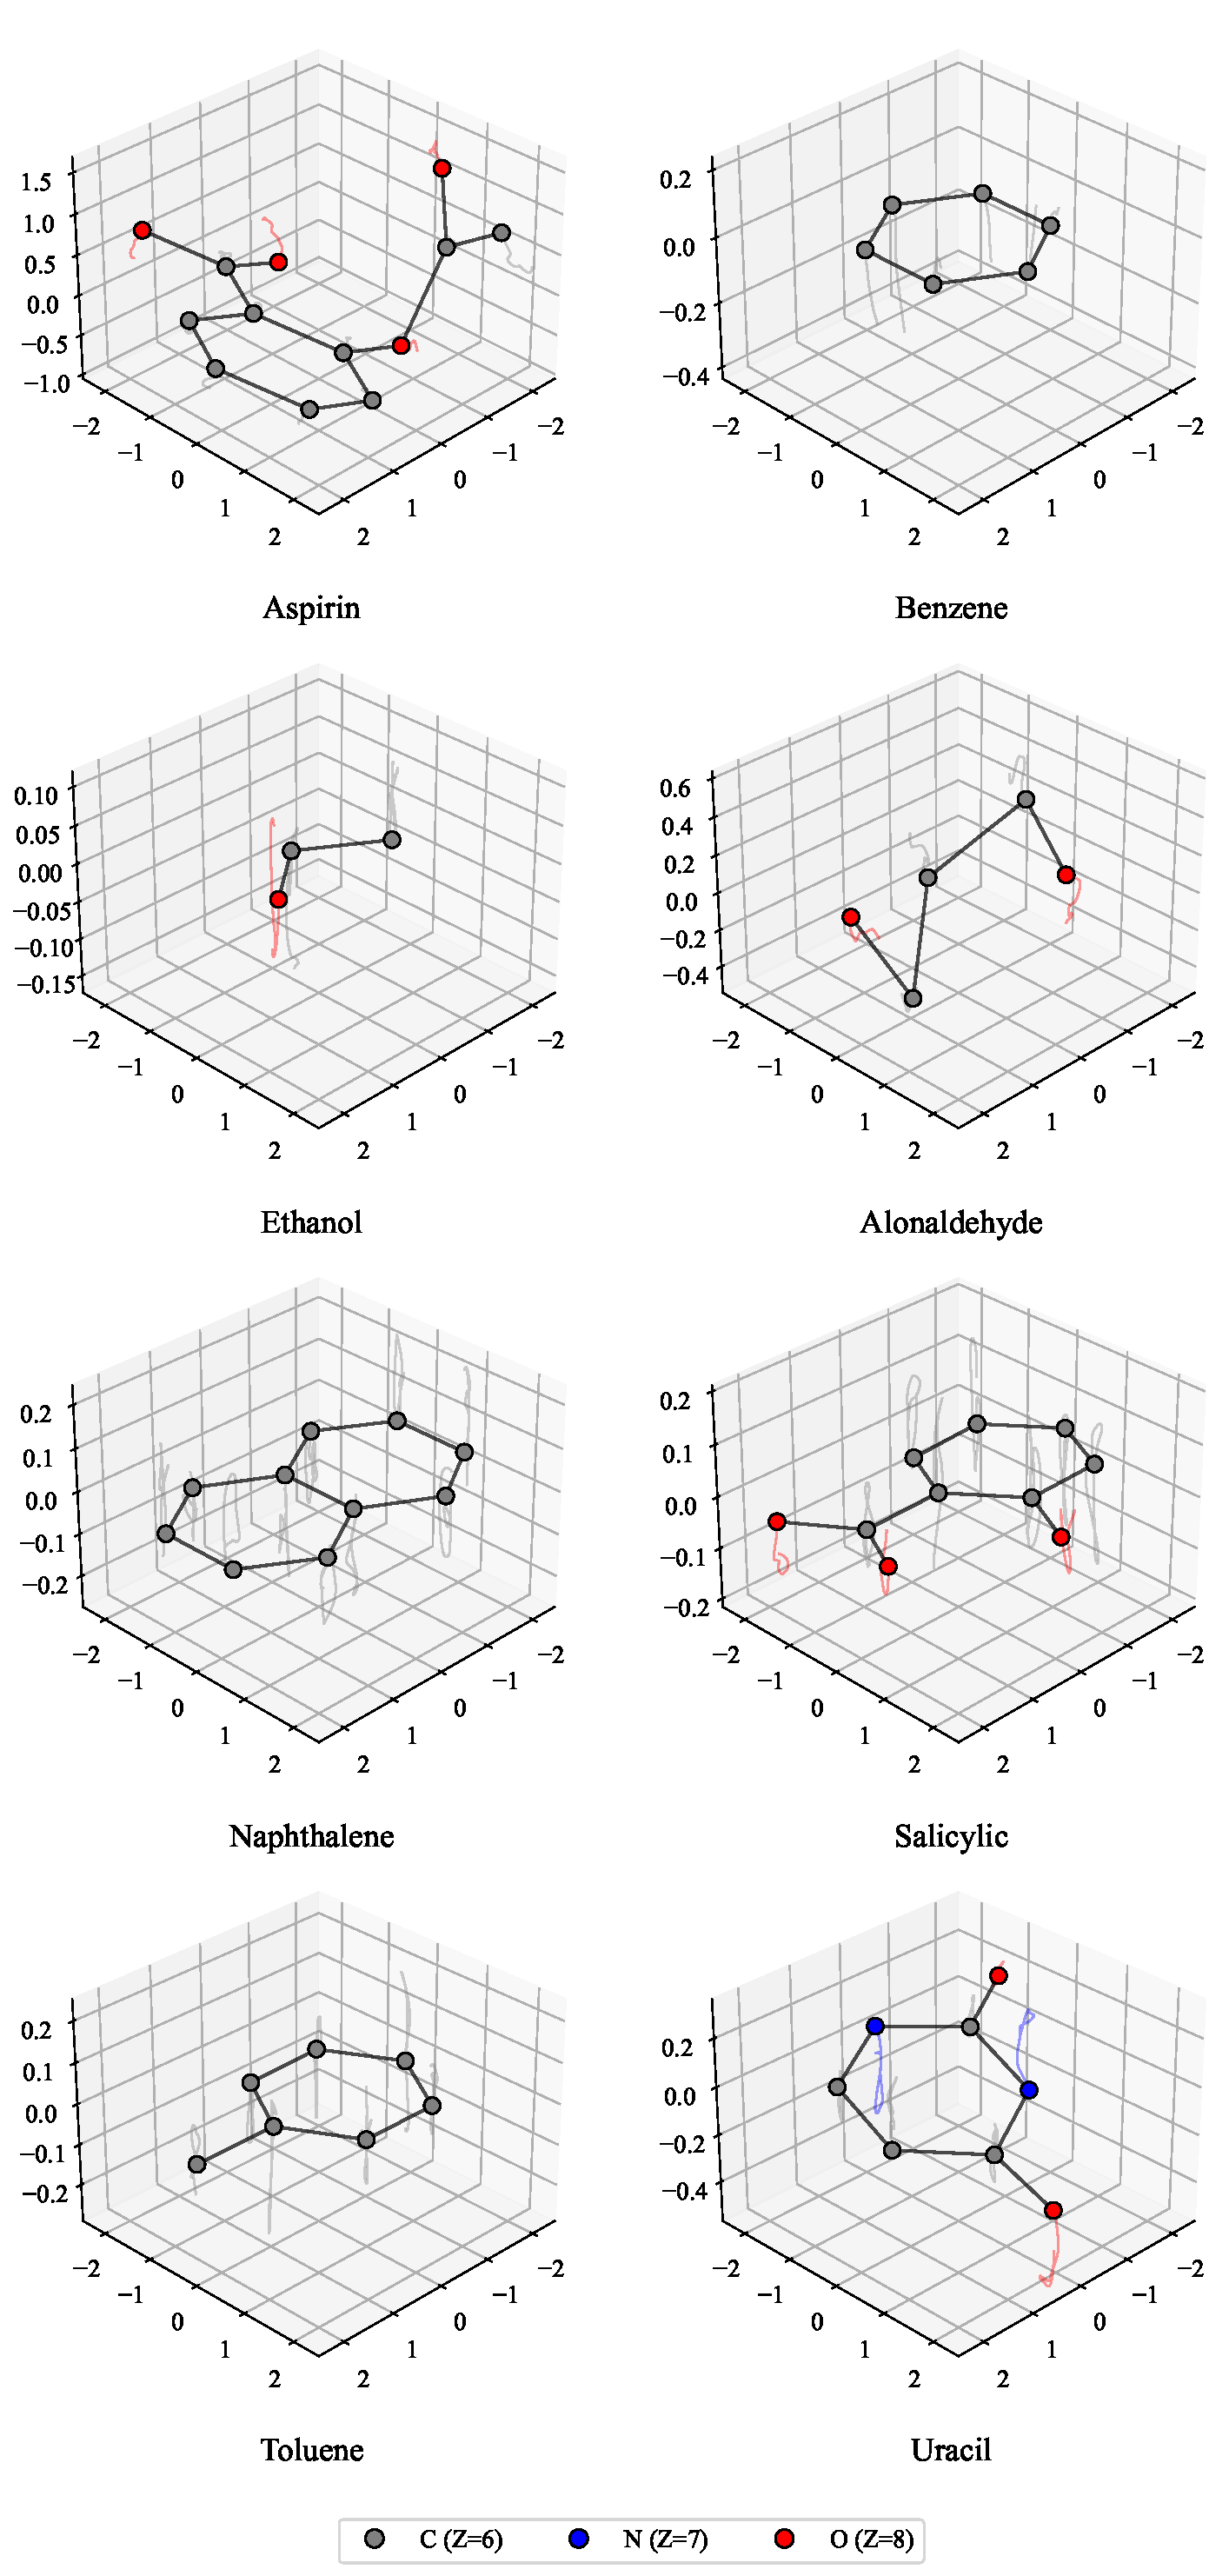
\includegraphics[width=\linewidth]{Figures/dataset/md17_combined_trajectories.pdf}
        \caption{MD17 trajectories}
        \label{fig:MD17_trajectories}
    \end{subfigure}
    \hfill
    \begin{subfigure}{0.48\linewidth}
        \centering
        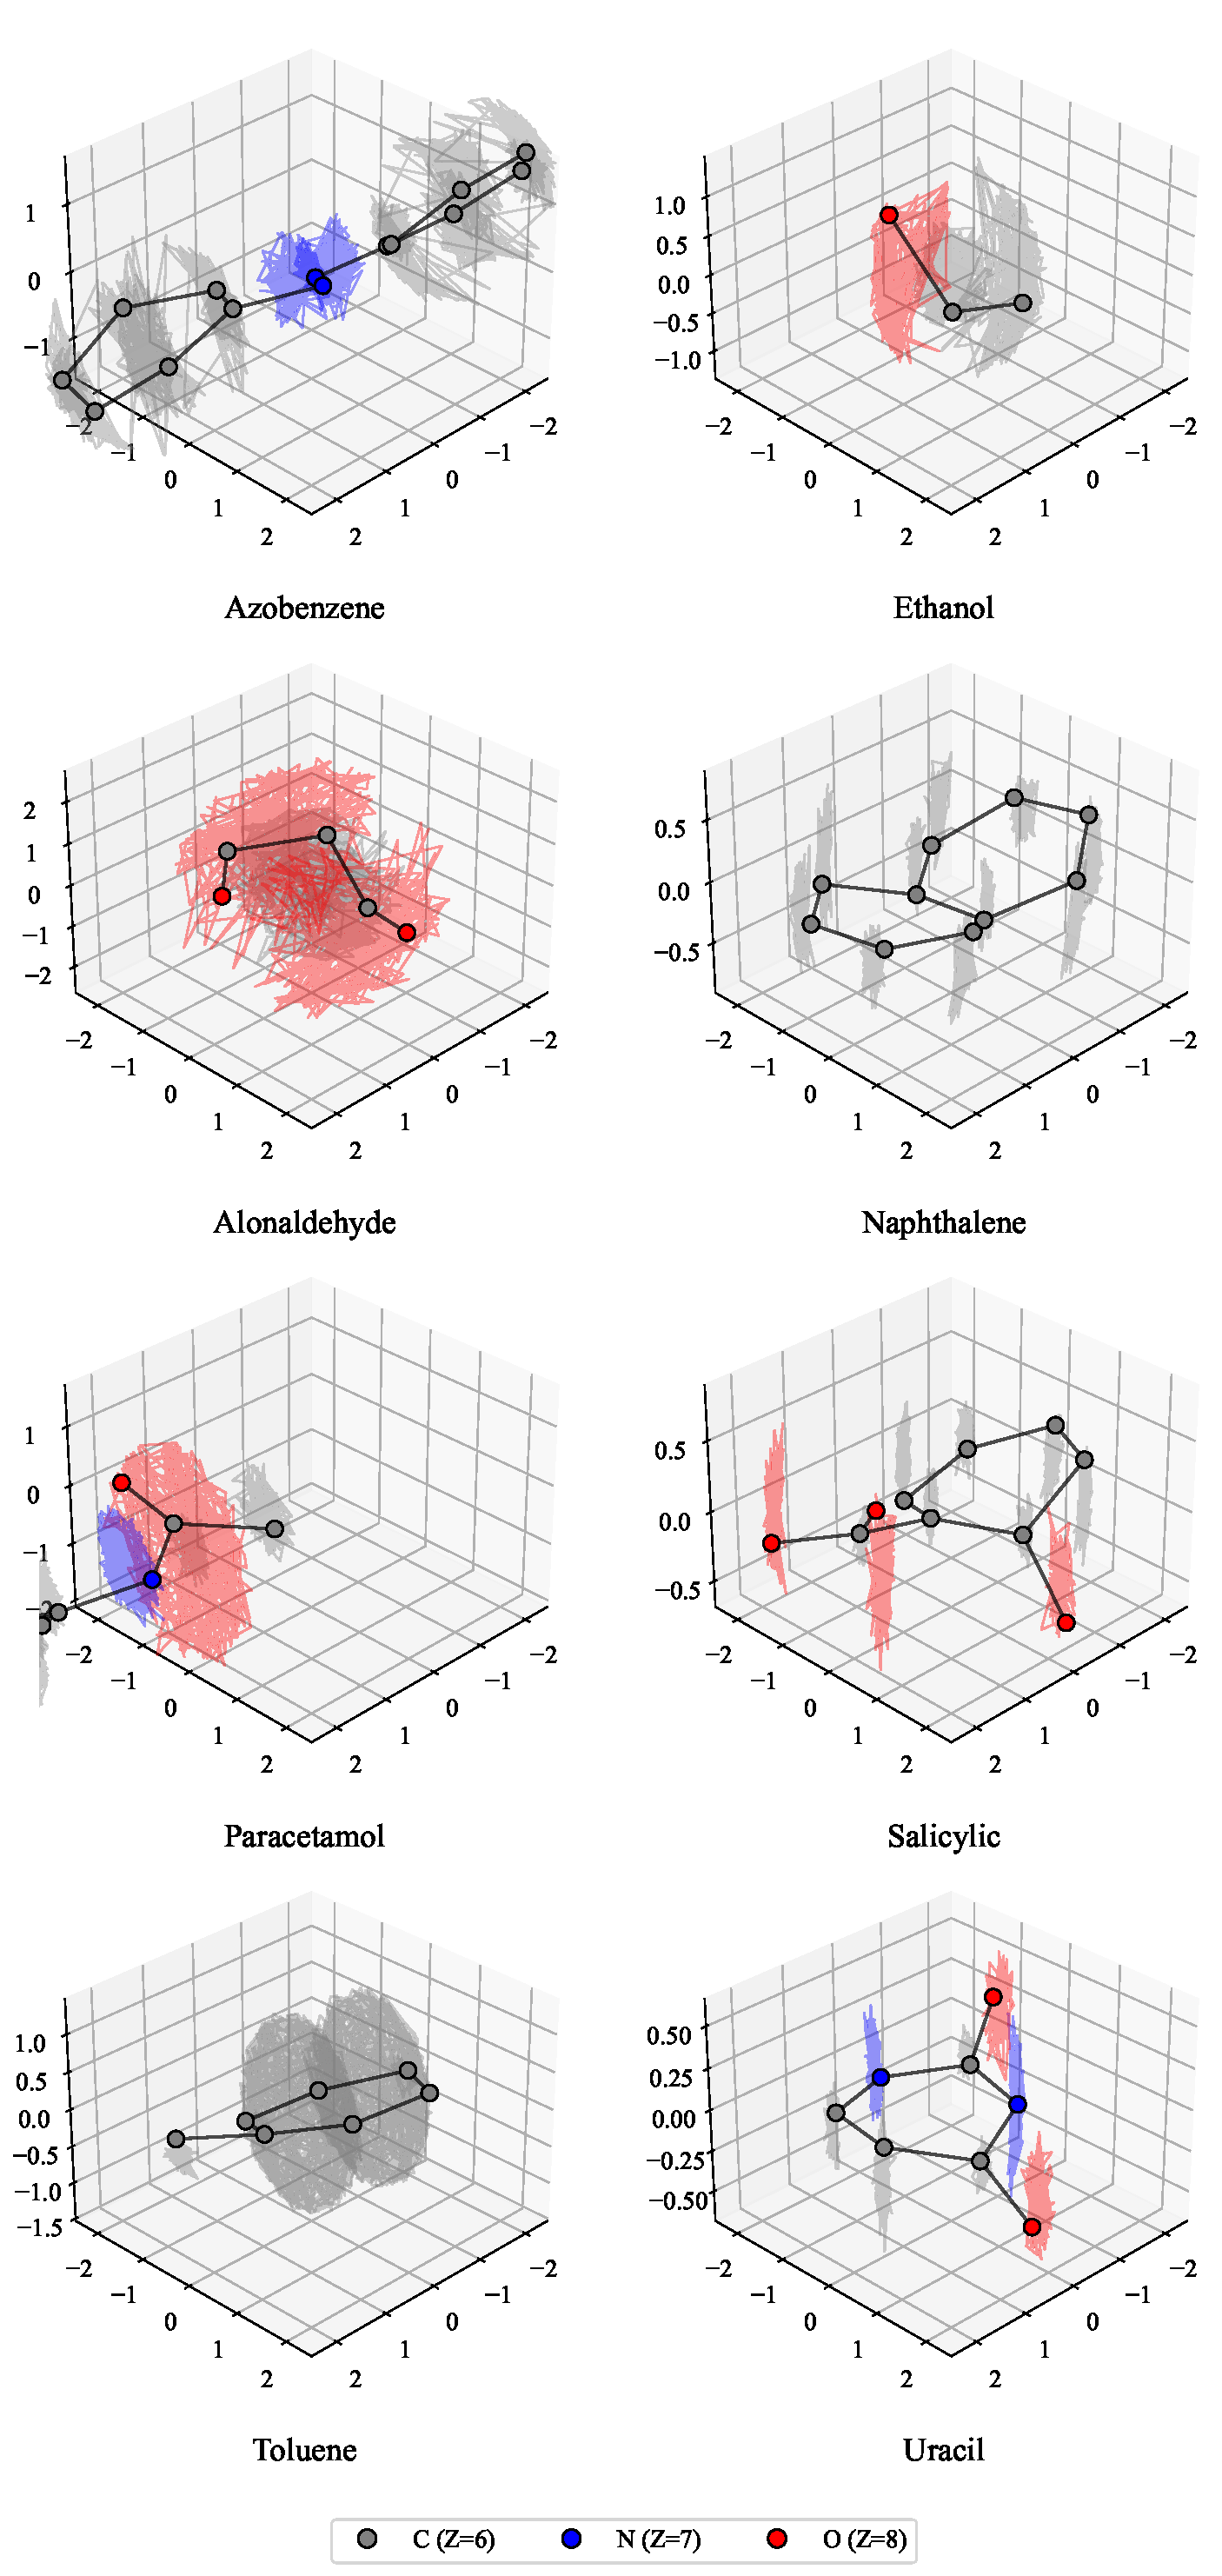
\includegraphics[width=\linewidth]{Figures/dataset/rmd17_combined_trajectories.pdf}
        \caption{RMD17 trajectories}
        \label{fig:RMD17_trajectories}
    \end{subfigure}
    \caption{3000 steps \gls{md} trajectories from the MD17 and RMD17 datasets.}
    \label{fig:trajectories}
\end{figure}
\newpage
\begin{figure}[H]
    \centering
    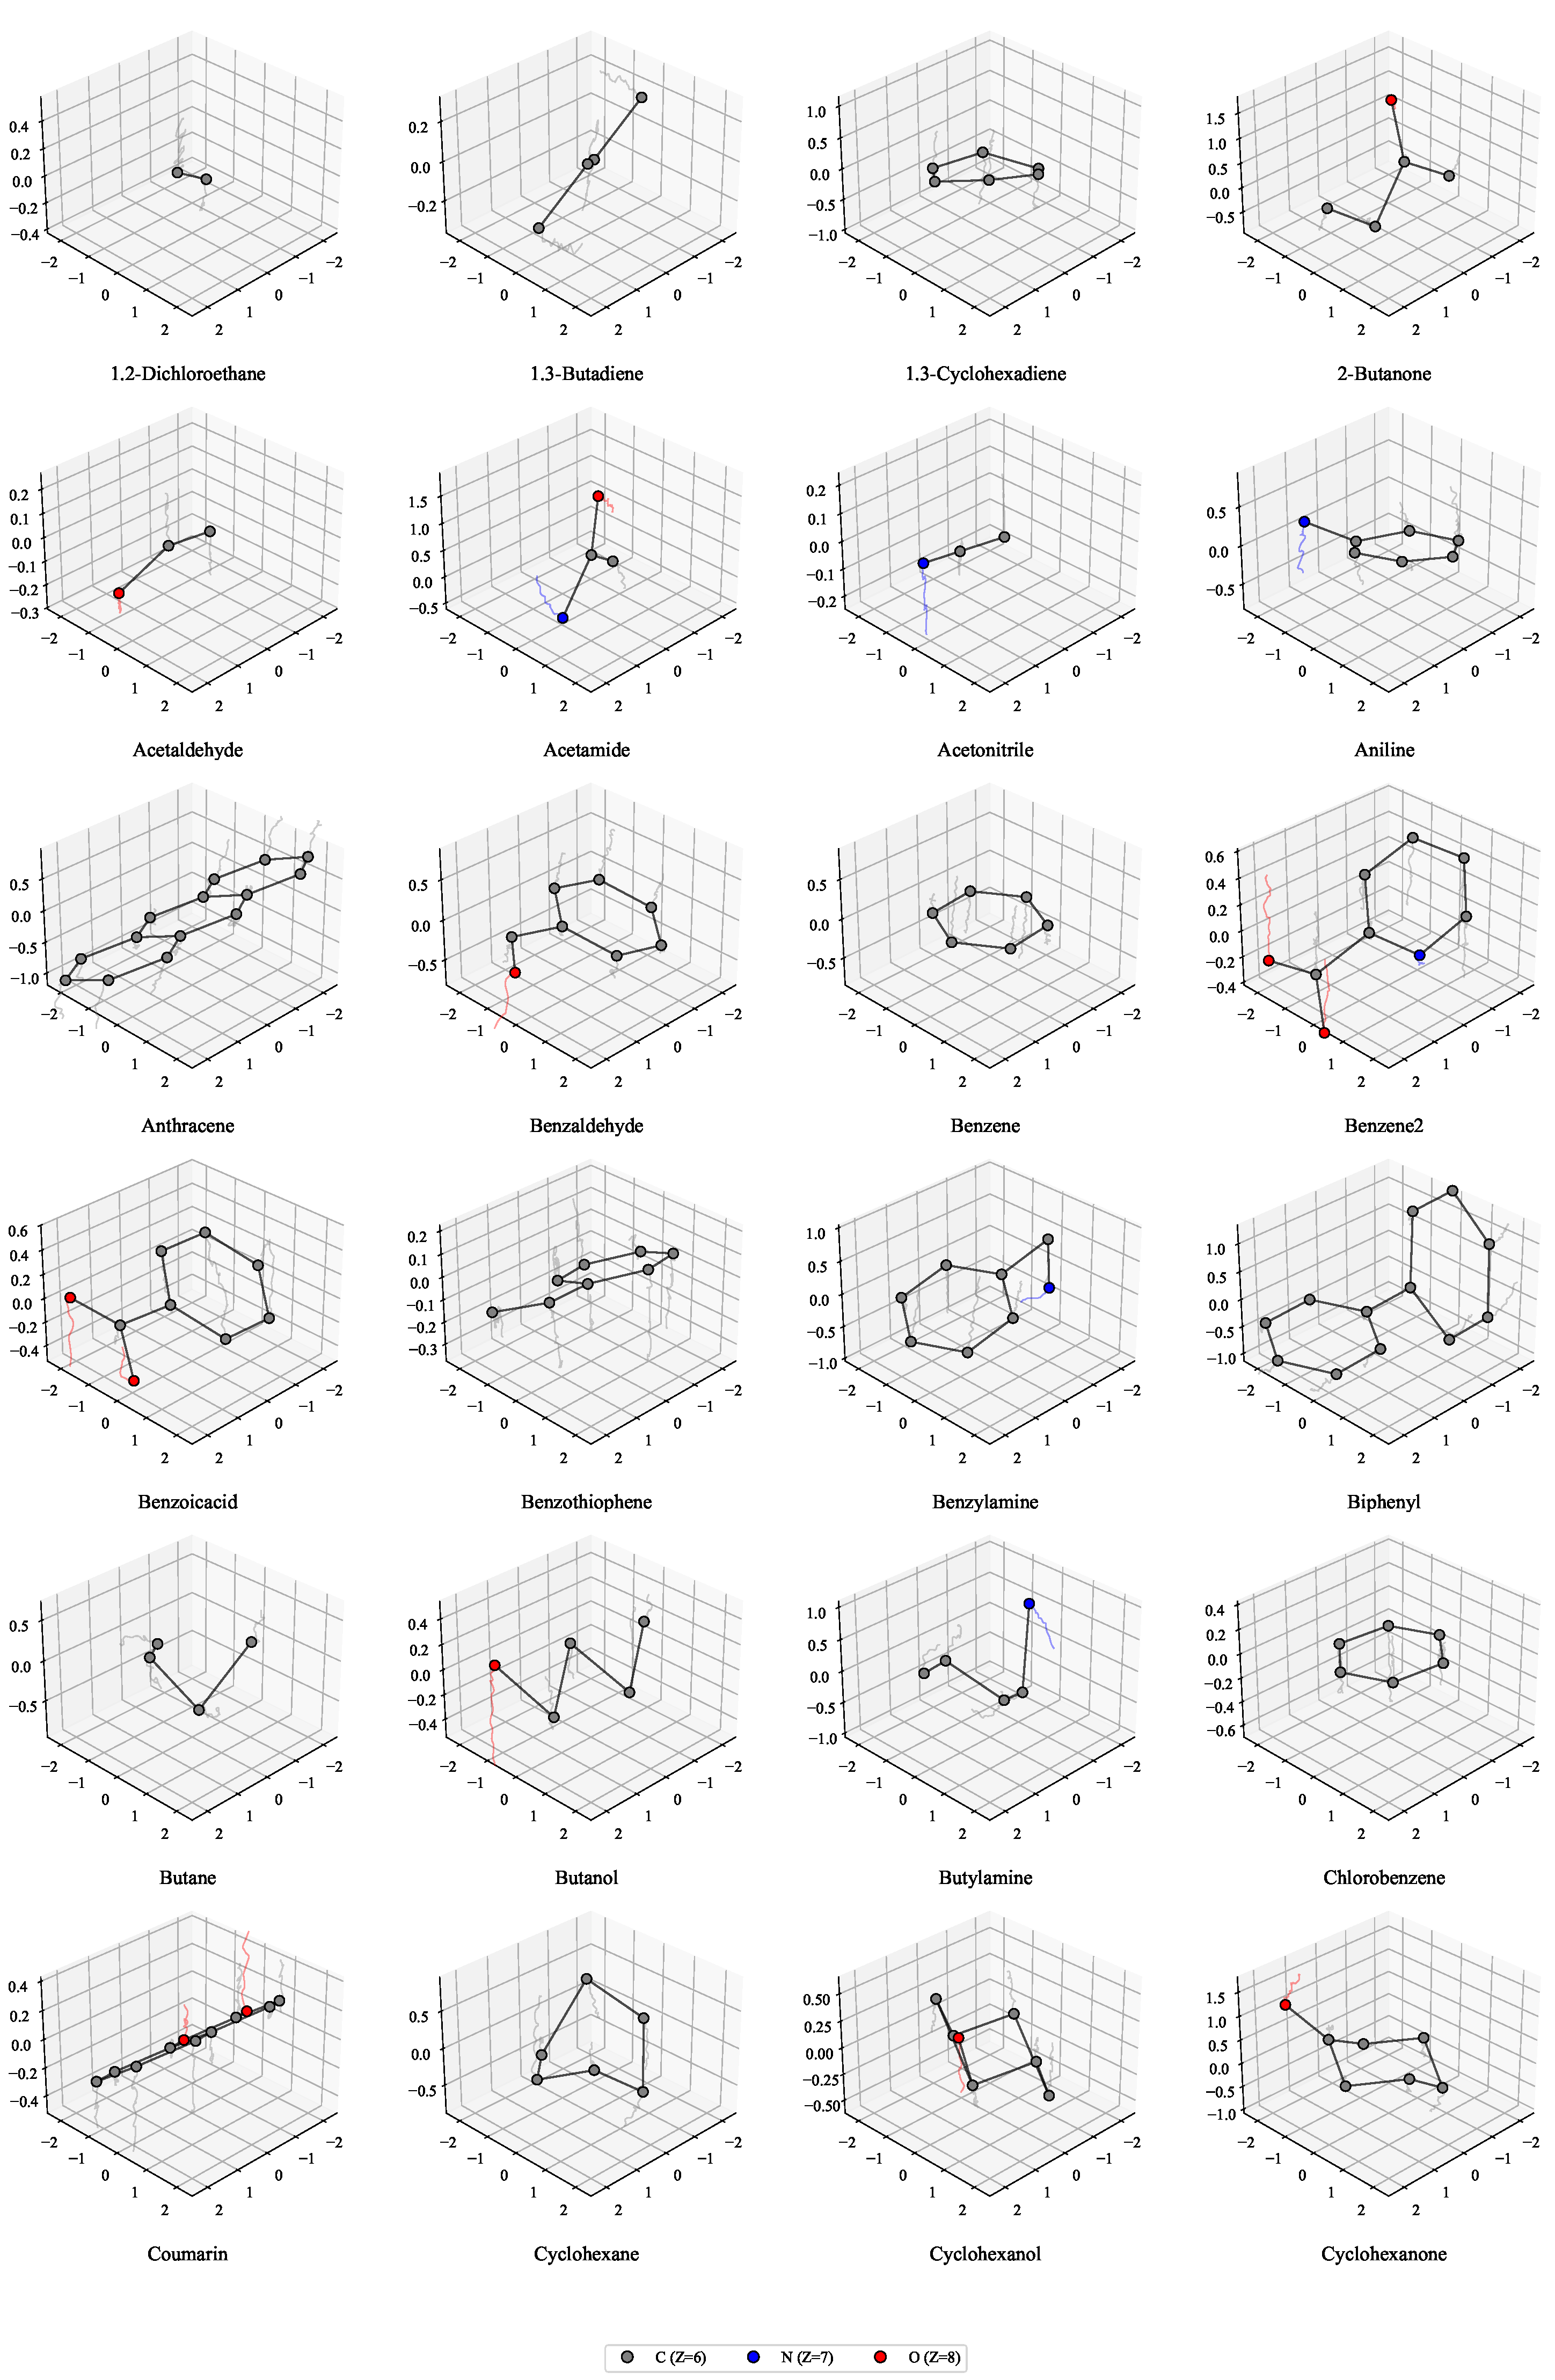
\includegraphics[width=\linewidth]{Figures/dataset/tg80_combined_trajectories_1.pdf}
    \label{fig:TG80_trajectories_1}
\end{figure}
\begin{figure}
    \centering
    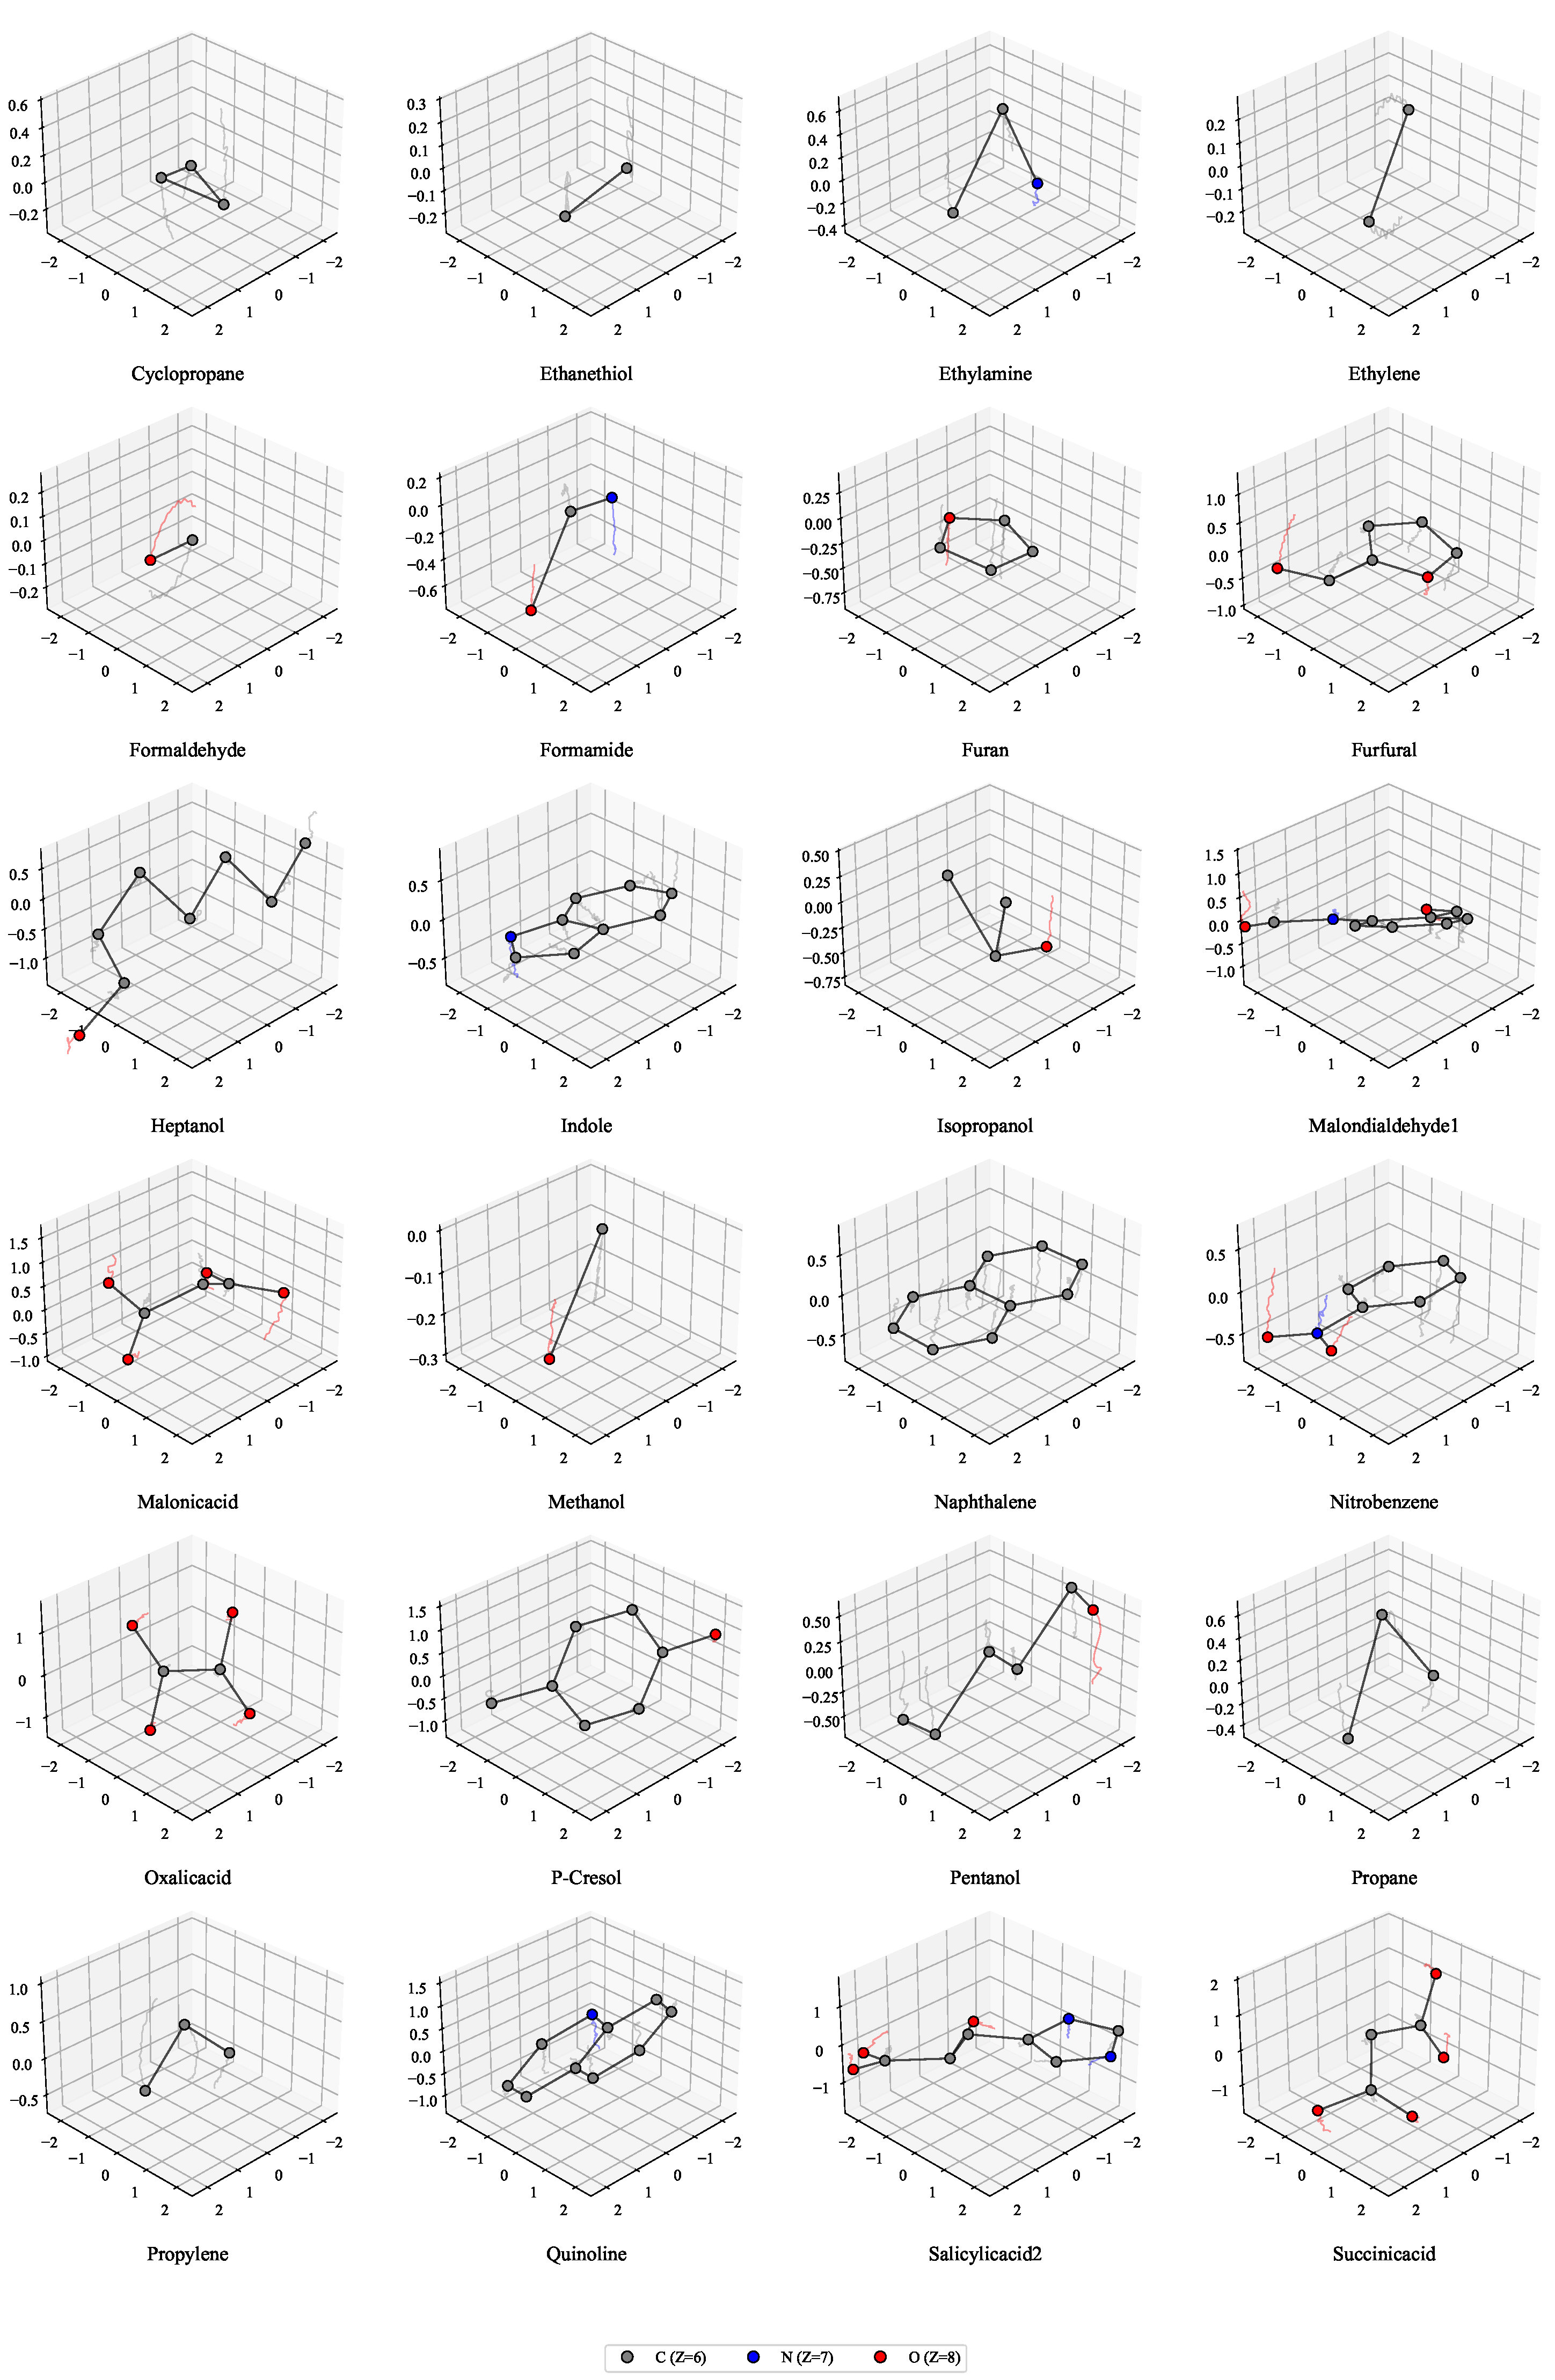
\includegraphics[width=\linewidth]{Figures/dataset/tg80_combined_trajectories_2.pdf}
    \label{fig:TG80_trajectories_2}
\end{figure}
\begin{figure}
    \centering
    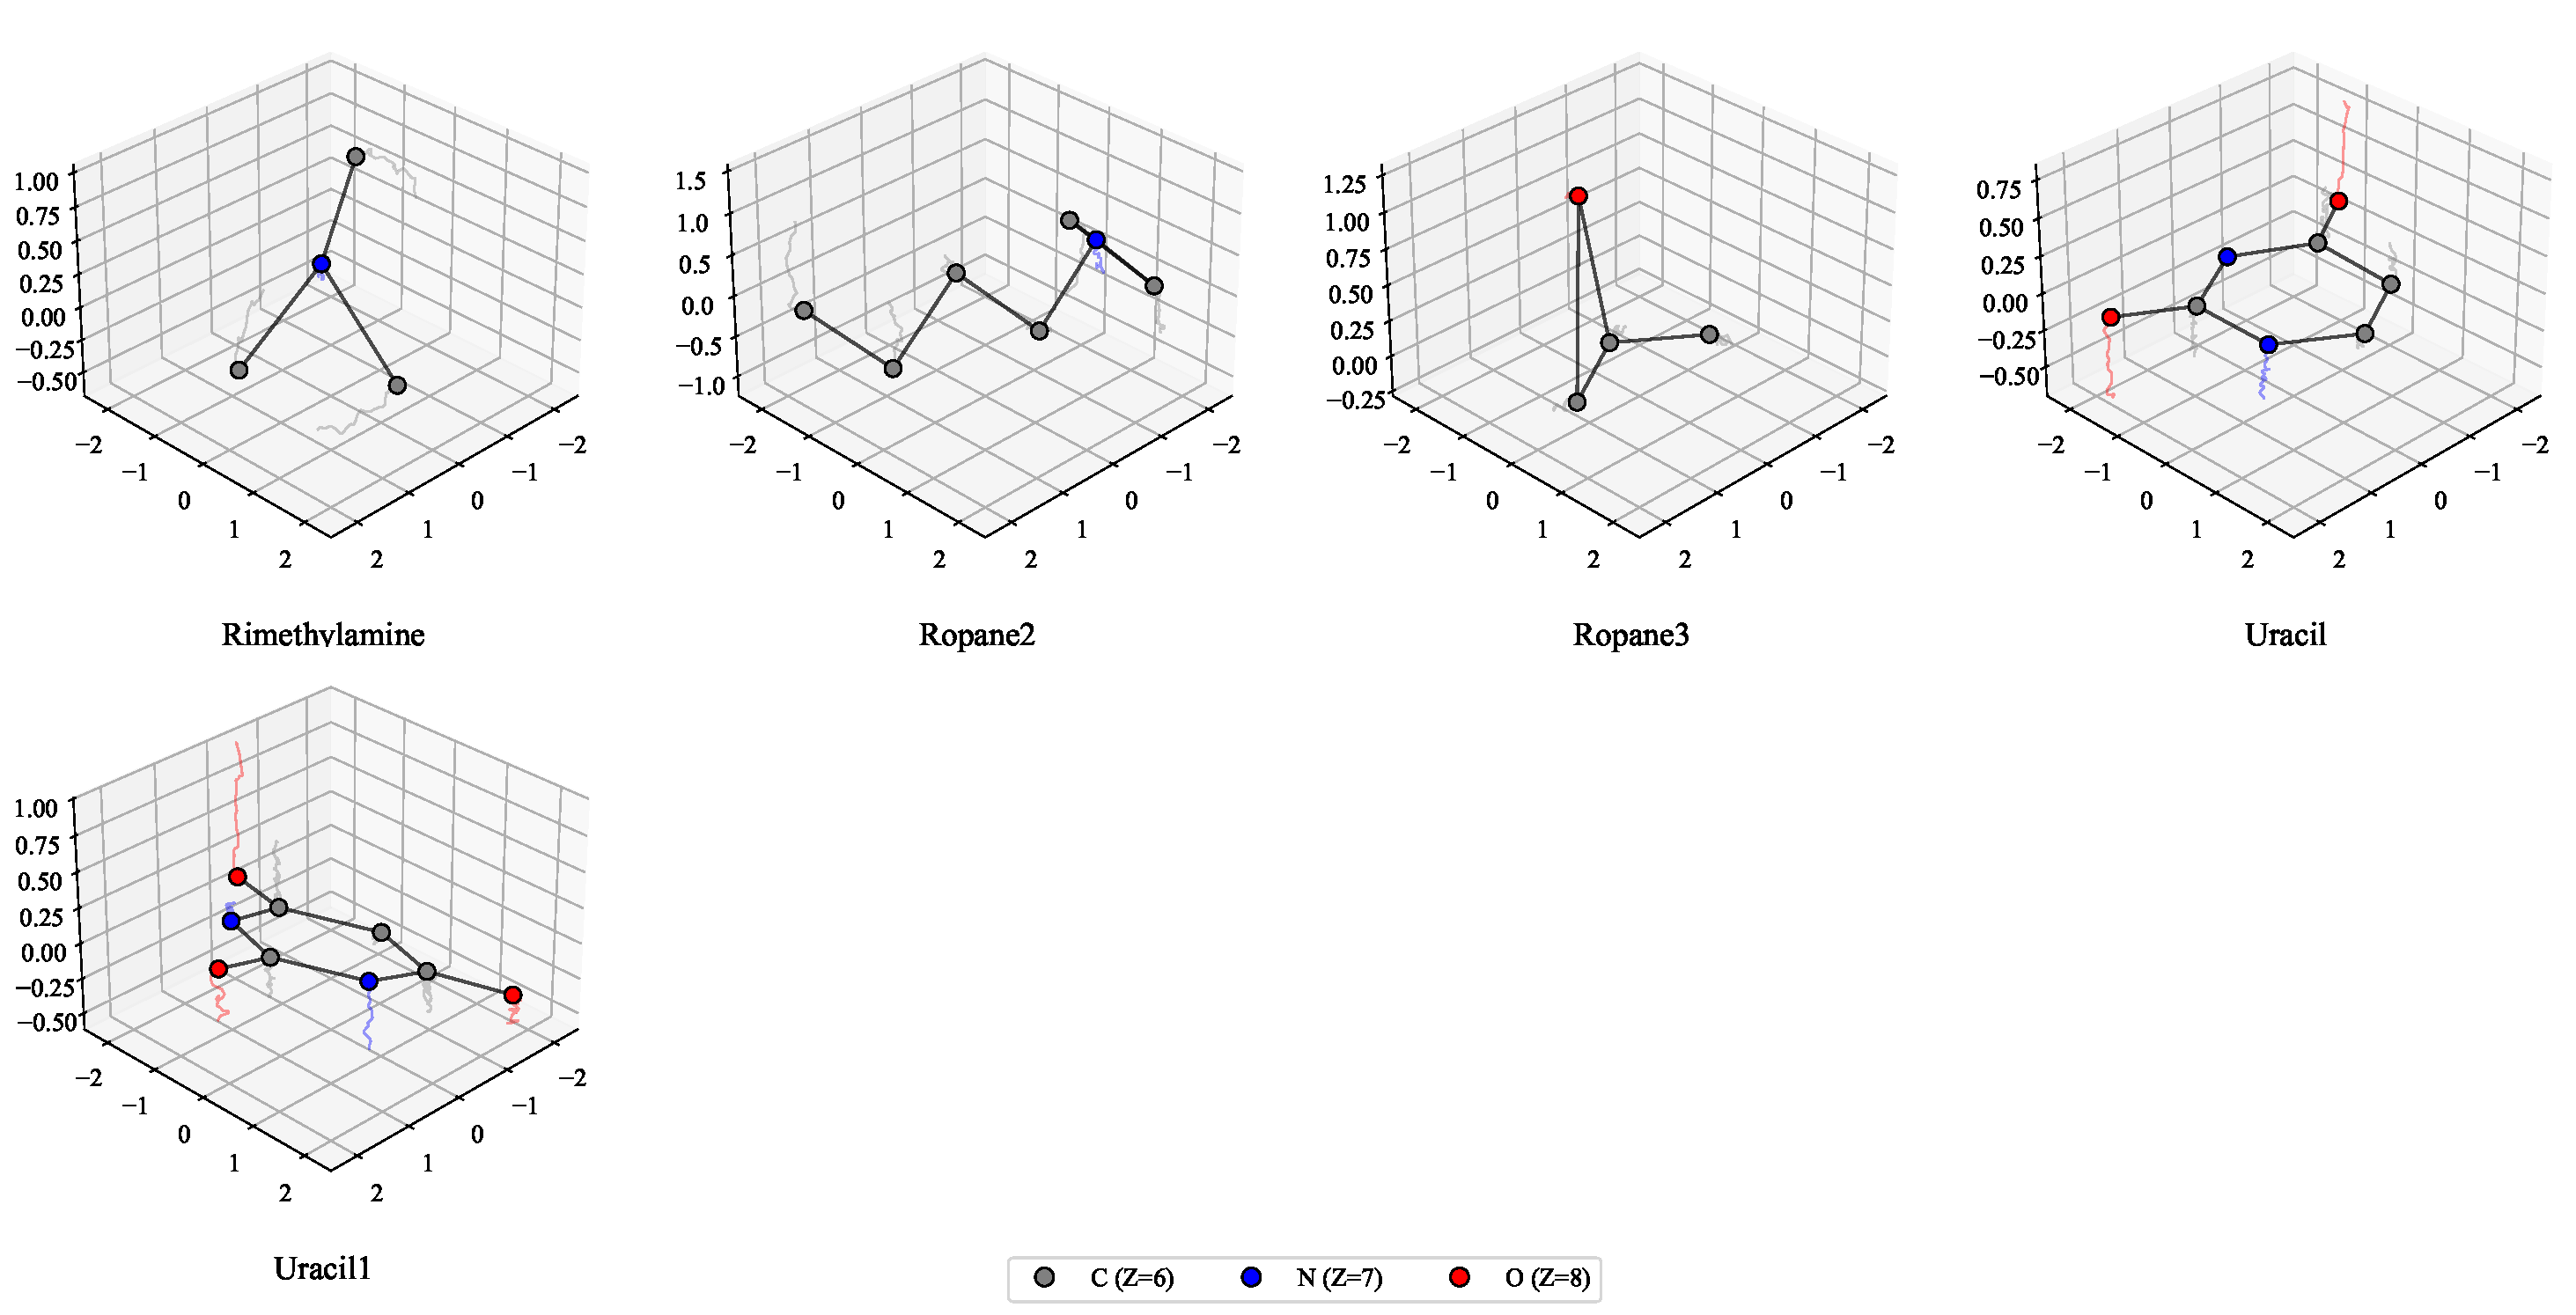
\includegraphics[width=\linewidth]{Figures/dataset/tg80_combined_trajectories_3.pdf}
    \label{fig:TG80_trajectories_3}
    \caption{3000-step \gls{md} trajectories from TG80. Molecules generated by our dataset expansion algorithm are named according to their seed molecule and the order of their selection.}
\end{figure}




\end{document}